\documentclass[12pt,a4paper]{report}
%DIF LATEXDIFF DIFFERENCE FILE
%DIF DEL expanded_old/expanded.tex   Fri Jan 15 18:13:20 2016
%DIF ADD expanded_new/expanded.tex   Fri Jan 15 18:49:29 2016


\usepackage[utf8]{inputenc}
\usepackage{amsmath}
\usepackage{amsfonts}
\usepackage{amssymb}
\usepackage{pgf}
\usepackage{graphicx}
\usepackage{amsthm}
\usepackage{natbib}
\usepackage{algorithm}
\usepackage{algpseudocode}
\usepackage{framed}
\usepackage{todonotes}
\usepackage[margin=0.7in]{geometry}
\usepackage{tcolorbox}
\tcbuselibrary{breakable}
\usepackage{caption}
\usepackage{sidecap}
\usepackage{listings}
\usepackage{afterpage}
%DIF 23d23
%DIF < \usepackage{ulem}
%DIF -------
\usepackage{fancyhdr}
\pagestyle{fancy}
%DIF 26a25
\usepackage{wasysym} %DIF > 
%DIF -------

\usepackage{hyperref}
\AtBeginDocument{\let\textlabel\label}
\hypersetup{
    colorlinks=true,
    linkcolor=black,
    citecolor=black,
    filecolor=black,
    urlcolor=black,
}
\usepackage{thmtools} 
\usepackage{marginnote}
\renewcommand*{\marginfont}{\scriptsize}
\marginparwidth=0.5in



\theoremstyle{plain}
\newtheorem{theorem}{Theorem}[section]
\newtheorem*{theorem*}{Theorem}
\newtheorem{lemma}{Lemma}[section]
\newtheorem*{lemma*}{Lemma}
\newtheorem{prop}{Proposition}[section]
\newtheorem{cor}{Corollary}[section]


\theoremstyle{definition}
\newtheorem{definition}{Definition}
\newtheorem{remark}{Remark}
\newtheorem{extra}{Extra Info}
\newtheorem{example}{Example}






\newcommand{\naive}{na\"{\i}ve }
\newcommand{\Naive}{Na\"{\i}ve }
\newcommand{\andor}{and\textbackslash or }
\newcommand{\erdos}{Erd\H{o}s }
\newcommand{\renyi}{R\`enyi }


\newcommand{\al}{\alpha}
\newcommand{\be}{\beta}
\newcommand{\si}{\sigma}

\newcommand{\set}[1]{\{ #1 \}} \newcommand{\setII}[1]{\left\{ #1 \right\}} \newcommand{\rv}[1]{\mathbf{#1}} \newcommand{\x}{\rv x} \newcommand{\y}{\rv y} \newcommand{\U}{\rv u} \newcommand{\T}{\rv t} \newcommand{\X}{\rv X} \newcommand{\Y}{\rv Y} \newcommand{\expect}[1]{\mathbf{E}\left[ #1 \right]} \newcommand{\expectg}[2]{\mathbf{E}_{\rv{#1}}\left[ \rv{#2} \right]} \newcommand{\expectn}[1]{\mathbb{E}\left[#1\right]} \newcommand{\cov}[1]{\mathbf{Cov} \left[ #1 \right]} \newcommand{\var}[1]{\mathop{Var} \left[ #1 \right]} \newcommand{\covn}[1]{\mathbb{Cov} \left[ #1 \right]} \newcommand{\gauss}[1]{\mathcal{N}\left(#1\right)} \newcommand{\cdf}[2]{F_{#1} (#2)} \newcommand{\survive}[2]{S_{#1} (#2)} \newcommand{\hazard}[2]{h_{#1} (#2)} \newcommand{\cuhazard}[2]{H_{#1} (#2)} \newcommand{\cdfn}[2]{\mathbb{F}_{#1}(#2)} \newcommand{\icdf}[2]{F_\rv{#1}^{-1} (#2)} \newcommand{\icdfn}[2]{\mathbb{F}^{-1}_{#1}(#2)} \newcommand{\pdf}[2]{p_{#1} (#2)} \newcommand{\prob}[1]{P\left( #1 \right)} \newcommand{\dist}{P} \newcommand{\density}{p}
\newcommand{\entropy}{H} \newcommand{\mutual}[2]{I\left(#1;#2\right)} 
\newcommand{\estim}[1]{\widehat{#1}} \newcommand{\estimII}[1]{\tilde{#1}} 
\newcommand{\norm}[1]{\Vert #1 \Vert} \newcommand{\normII}[1]{\norm{#1}_2} \newcommand{\normI}[1]{\norm{#1}_1} \newcommand{\normF}[1]{\norm{#1}_{Frob}} \newcommand{\ones}{\textbf{1}} \newcommand{\lik}{\mathcal{L}} \newcommand{\loglik}{L} \newcommand{\loss}{l} \newcommand{\lossII}{\prescript{}{2}{l}} \newcommand{\risk}{R} \newcommand{\riskn}{\mathbb{R}} \newcommand{\riskII}{\prescript{}{2}{R}} \newcommand{\risknII}{\prescript{}{2}{\mathbb{R}} } \newcommand{\noisen}{\mathbb{G}} \newcommand{\deriv}[2]{\frac{\partial #1}{\partial #2}} \newcommand{\argmin}[2]{\textstyle{\mathop{argmin}_{#1}}\set{#2}} \newcommand{\argmax}[2]{\textstyle{\mathop{argmax}_{#1}}\set{#2}} \newcommand{\hyp}{f} \newcommand{\hypclass}{\mathcal{F}} \newcommand{\hilbert}{\mathcal{H}}
\newcommand{\rkhs}{\hilbert_\kernel} \newcommand{\normrkhs}[1]{\norm{#1}_{\rkhs}} 

\newcommand{\plane}{\mathbb{L}} \newcommand{\categories}{\mathcal{G}} \newcommand{\positive}[1]{\left[ #1 \right]_+} \newcommand{\kernel}{\mathcal{K}} \newcommand{\featureS}{\mathcal{X}} \newcommand{\outcomeS}{\mathcal{Y}} \newcommand{\indicator}[1]{I_{\set{#1}}} \newcommand{\reals}{\mathbb{R}} 


\newcommand{\latent}{\rv{s}} \newcommand{\latentn}{S} \newcommand{\loadings}{A} \newcommand{\rotation}{R}  \newcommand{\similaritys}{\mathfrak{S}} \newcommand{\similarity}{s} \newcommand{\dissimilarity}{d} \newcommand{\dissimilaritys}{\mathfrak{D}} \newcommand{\scalar}[2]{\left< #1,#2 \right>} 


\newcommand{\manifold}{\mathcal{M}} \newcommand{\project}{\hookrightarrow} \newcommand{\projectMat}{H} \newcommand{\rank}{q} \newcommand{\dimy}{K} \newcommand{\encode}{E} \newcommand{\decode}{D} \DeclareMathOperator{\Tr}{Tr}
\newcommand{\ensembleSize}{M} \newcommand{\ensembleInd}{m} 

\newcommand{\sample}{\mathcal{S}} \newcommand{\test}{\risk(\hyp)} \newcommand{\train}{\riskn(\hyp)} \newcommand{\insample}{\bar{\risk}(\hyp)} \newcommand{\EPE}{\risk(\hat{\hyp}_n)} \newcommand{\folds}{K} \newcommand{\fold}{k} \newcommand{\bootstraps}{B} \newcommand{\bootstrap}{{b^*}} 

\newcommand{\rankings}{\mathcal{R}} \newcommand{\ranking}{\mathcal{R}} \newcommand{\KL}[2]{D_{KL}\left(#1 \Vert #2 \right)}
\newcommand{\ortho}{\mathbb{O}} 
\newcommand{\id}[6]{
	\begin{tabular}{|p{2cm}|p{2cm}|p{2cm}|p{2cm}|p{2cm}|p{2cm}|}
	\hline Task & Type & Input & Output & Concept & Remark \\ 
	\hline 
	\hline #1 & #2 & #3 & #4 & #5 & #6 \\ 
	\hline 
	\end{tabular} 
	\newline
	\newline
}

\newcommand{\union}{\cup}
\newcommand{\intersect}{\cap}
\newcommand{\supp}[1]{\mathop{support}(#1)}
\newcommand{\conf}[2]{\mathop{confidence}(#1 \Rightarrow #2)}
\newcommand{\lift}[2]{\mathop{lift}(#1 \Rightarrow #2)}
\newcommand{\convic}[2]{\mathop{conviction}(#1 \Rightarrow #2)}


\newcommand{\machine}[1]{\estim{\theta}_n^{(#1)}}
\newcommand{\minimizer}{\theta^*}
\newcommand{\generative}{\theta_0}
\newcommand{\parallelized}{\bar{\theta}_{N,m}}
\newcommand{\parallelizedII}{\mathring{\theta}_{N,m}}
\newcommand{\parallelizedIII}{\prescript{}{2}{\widehat{\theta}}_{N,m}}
\newcommand{\centralized}{\estim{\theta}_N}
\newcommand{\parallelKL}{\estim{\theta}_{KL}}
\newcommand{\penalize}{J}
\newcommand{\bigO}{\mathcal{O}}
\newcommand{\bigOprob}{\mathcal{O}_P}
\newcommand{\smallO}{o}
\newcommand{\smallOprob}{o_P}

\newcommand{\citeJR}[1]{\citeauthor{#1} \citep{#1}}
\newcommand{\citeJRfull}[1]{\citeauthor*{#1} \citep{#1}}
\newcommand{\error}{\mathcal{E}}

\newcommand{\M}{$M$}
\newcommand{\MII}{$\prescript{}{2}{M}$}

\newcommand{\biasSecond}[1]{B_2(#1)}
\newcommand{\MSESecond}[1]{M_2(#1)}

\newcommand{\rate}{r}

\newcommand{\emptyfigure}[1]{\missingfigure[figwidth=6cm]{#1}}



\usepackage{tikz}
\usetikzlibrary{arrows, calc, decorations.markings, positioning}


\makeatletter
\newenvironment{timeline}[6]{                        
    \newcommand{\startyear}{#1}
    \newcommand{\tlendyear}{#2}

    \newcommand{\yearcolumnwidth}{#3}
    \newcommand{\rulecolumnwidth}{#4}
    \newcommand{\entrycolumnwidth}{#5}
    \newcommand{\timelineheight}{#6}

    \newcommand{\templength}{}

    \newcommand{\entrycounter}{0}

            \long\def\ifnodedefined##1##2##3{        \@ifundefined{pgf@sh@ns@##1}{##3}{##2}    }

    \newcommand{\ifnodeundefined}[2]{        \ifnodedefined{##1}{}{##2}
    }

    \newcommand{\drawtimeline}{        \draw[timelinerule] (\yearcolumnwidth+5pt, 0pt) -- (\yearcolumnwidth+5pt, -\timelineheight);
        \draw (\yearcolumnwidth+0pt, -10pt) -- (\yearcolumnwidth+10pt, -10pt);
        \draw (\yearcolumnwidth+0pt, -\timelineheight+15pt) -- (\yearcolumnwidth+10pt, -\timelineheight+15pt);

        \pgfmathsetlengthmacro{\templength}{neg(add(multiply(subtract(\startyear, \startyear), divide(subtract(\timelineheight, 25), subtract(\tlendyear, \startyear))), 10))}
        \node[year] (year-\startyear) at (\yearcolumnwidth, \templength) {\startyear};

        \pgfmathsetlengthmacro{\templength}{neg(add(multiply(subtract(\tlendyear, \startyear), divide(subtract(\timelineheight, 25), subtract(\tlendyear, \startyear))), 10))}
        \node[year] (year-\tlendyear) at (\yearcolumnwidth, \templength) {\tlendyear};
    }

    \newcommand{\entry}[2]{                
        \pgfmathtruncatemacro{\lastentrycount}{\entrycounter}
        \pgfmathtruncatemacro{\entrycounter}{\entrycounter + 1}

        \ifdim \lastentrycount pt > 0 pt            \node[entry] (entry-\entrycounter) [below of=entry-\lastentrycount] {##2};
        \else            \pgfmathsetlengthmacro{\templength}{neg(add(multiply(subtract(\startyear, \startyear), divide(subtract(\timelineheight, 25), subtract(\tlendyear, \startyear))), 10))}
            \node[entry] (entry-\entrycounter) at (\yearcolumnwidth+\rulecolumnwidth+10pt, \templength) {##2};
        \fi

        \ifnodeundefined{year-##1}{            \pgfmathsetlengthmacro{\templength}{neg(add(multiply(subtract(##1, \startyear), divide(subtract(\timelineheight, 25), subtract(\tlendyear, \startyear))), 10))}
            \draw (\yearcolumnwidth+2.5pt, \templength) -- (\yearcolumnwidth+7.5pt, \templength);
            \node[year] (year-##1) at (\yearcolumnwidth, \templength) {##1};
        }

        \draw ($(year-##1.east)+(2.5pt, 0pt)$) -- ($(year-##1.east)+(7.5pt, 0pt)$) -- ($(entry-\entrycounter.west)-(5pt,0)$) -- (entry-\entrycounter.west);
    }

    \newcommand{\plainentry}[2]{                
        \pgfmathtruncatemacro{\lastentrycount}{\entrycounter}
        \pgfmathtruncatemacro{\entrycounter}{\entrycounter + 1}

        \ifdim \lastentrycount pt > 0 pt            \node[entry] (entry-\entrycounter) [below of=entry-\lastentrycount] {##2};
        \else            \pgfmathsetlengthmacro{\templength}{neg(add(multiply(subtract(\startyear, \startyear), divide(subtract(\timelineheight, 25), subtract(\tlendyear, \startyear))), 10))}
            \node[entry] (entry-\entrycounter) at (\yearcolumnwidth+\rulecolumnwidth+10pt, \templength) {##2};
        \fi

        \ifnodeundefined{invisible-year-##1}{            \pgfmathsetlengthmacro{\templength}{neg(add(multiply(subtract(##1, \startyear), divide(subtract(\timelineheight, 25), subtract(\tlendyear, \startyear))), 10))}
            \draw (\yearcolumnwidth+2.5pt, \templength) -- (\yearcolumnwidth+7.5pt, \templength);
            \node[year] (invisible-year-##1) at (\yearcolumnwidth, \templength) {};
        }

        \draw ($(invisible-year-##1.east)+(2.5pt, 0pt)$) -- ($(invisible-year-##1.east)+(7.5pt, 0pt)$) -- ($(entry-\entrycounter.west)-(5pt,0)$) -- (entry-\entrycounter.west);
    }

    \begin{tikzpicture}
        \tikzstyle{entry} = [            align=left,            text width=\entrycolumnwidth,            node distance=10mm,            anchor=west]
        \tikzstyle{year} = [anchor=east]
        \tikzstyle{timelinerule} = [            draw,            decoration={markings, mark=at position 1 with {\arrow[scale=1.5]{latex'}}},            postaction={decorate},            shorten >=0.4pt]

        \drawtimeline
}
{
    \end{tikzpicture}
    \let\startyear\@undefined
    \let\tlendyear\@undefined
    \let\yearcolumnwidth\@undefined
    \let\rulecolumnwidth\@undefined
    \let\entrycolumnwidth\@undefined
    \let\timelineheight\@undefined
    \let\entrycounter\@undefined
    \let\ifnodedefined\@undefined
    \let\ifnodeundefined\@undefined
    \let\drawtimeline\@undefined
    \let\entry\@undefined
}
\makeatother

\newcommand{\R}{\textnormal{\sffamily\bfseries R }}

\newcommand{\targetValue}{T}\newcommand{\cp}{C_p}\newcommand{\cpHat}{\hat{C}_p}\newcommand{\ctqExpect}{\mu}
\newcommand{\pnc}{p_{NC}}
\newcommand{\cpu}{C_{pu}}
\newcommand{\cpl}{C_{pl}}
\newcommand{\cpk}{C_{pk}}
\newcommand{\cpm}{C_{pm}}
\newcommand{\cpq}{C_p(q)}
\newcommand{\pp}{P_{p}}
\newcommand{\ppk}{P_{pk}}

\newcommand{\barxChart}{$\bar{x}$-chart }
\newcommand{\sigmabar}{\sigma_{\bar{x}}}
\newcommand{\aka}{{a.k.a.\ }}
\newcommand{\Aka}{{A.k.a.\ }}
\newcommand{\rcode}[1]{\texttt{#1}}
\newcommand{\arm}{L}

\newcommand{\tsq}{$T^2_t$ }
\newcommand{\struct}{\Phi}
\newcommand{\exppdf}[2]{#1 e^{-#1 #2}}
\newcommand{\expcdf}[2]{e^{-#1 #2}}

\newcommand{\conv}{\ast}
 

\author{Jonathan Rosenblatt}
\title{Quality Engineering - Class Notes (experimental)}
%DIF PREAMBLE EXTENSION ADDED BY LATEXDIFF
%DIF UNDERLINE PREAMBLE %DIF PREAMBLE
\RequirePackage[normalem]{ulem} %DIF PREAMBLE
\RequirePackage{color}\definecolor{RED}{rgb}{1,0,0}\definecolor{BLUE}{rgb}{0,0,1} %DIF PREAMBLE
\providecommand{\DIFaddtex}[1]{{\protect\color{blue}\uwave{#1}}} %DIF PREAMBLE
\providecommand{\DIFdeltex}[1]{{\protect\color{red}\sout{#1}}}                      %DIF PREAMBLE
%DIF SAFE PREAMBLE %DIF PREAMBLE
\providecommand{\DIFaddbegin}{} %DIF PREAMBLE
\providecommand{\DIFaddend}{} %DIF PREAMBLE
\providecommand{\DIFdelbegin}{} %DIF PREAMBLE
\providecommand{\DIFdelend}{} %DIF PREAMBLE
%DIF FLOATSAFE PREAMBLE %DIF PREAMBLE
\providecommand{\DIFaddFL}[1]{\DIFadd{#1}} %DIF PREAMBLE
\providecommand{\DIFdelFL}[1]{\DIFdel{#1}} %DIF PREAMBLE
\providecommand{\DIFaddbeginFL}{} %DIF PREAMBLE
\providecommand{\DIFaddendFL}{} %DIF PREAMBLE
\providecommand{\DIFdelbeginFL}{} %DIF PREAMBLE
\providecommand{\DIFdelendFL}{} %DIF PREAMBLE
%DIF END PREAMBLE EXTENSION ADDED BY LATEXDIFF
%DIF PREAMBLE EXTENSION ADDED BY LATEXDIFF
%DIF HYPERREF PREAMBLE %DIF PREAMBLE
\providecommand{\DIFadd}[1]{\texorpdfstring{\DIFaddtex{#1}}{#1}} %DIF PREAMBLE
\providecommand{\DIFdel}[1]{\texorpdfstring{\DIFdeltex{#1}}{}} %DIF PREAMBLE
%DIF END PREAMBLE EXTENSION ADDED BY LATEXDIFF

\begin{document}

\maketitle


\chapter*{Preface}
This text accompanies my Quality Engineering course at the Dept. of Industrial Engineering at the Ben-Gurion University of the Negev.
It has several purposes:
\begin{itemize}
\item Help me organize and document the course material.
\item Help students during class so that they may focus on listening and not writing.
\item Help students after class, so that they may self-study.
\end{itemize}

At its current state it is experimental. It can thus be expected to change from time to time, and include mistakes.
I will be enormously grateful to whoever decides to share with me any mistakes found.

I also ask for the readers' forgiveness for my Wikipedia quoting style. 
It is highly unorthodox to cite Wikipedia as one would cite a peer reviewed publication. 
I do so, in this text, merely for technical convenience. 

I hope the reader will find this text interesting and useful. 




\tableofcontents

\listoffigures

\renewcommand{\listtheoremname}{List of Definitions}
\listoftheorems[ignoreall,show={definition}]






\chapter{Introduction}
\label{sec:introduction}

Quality Engineering is the study and design of practices aimed improving the ``quality'' of production. 
Production is understood in a wide sense, and includes services as well.
Quality is understood in many senses. Here are several definitions compiled verbatim from \cite{montgomery_introduction_2007}  and \cite{wikipedia_quality_2015}:
\begin{enumerate}
\item Montgomery: ``The reciprocal of variability''.
\item American Society for Quality:
A combination of quantitative and qualitative perspectives for which each person has his or her own definition; examples of which include, ``Meeting the requirements and expectations in service or product that were committed to'' and ``Pursuit of optimal solutions contributing to confirmed successes, fulfilling accountabilities.
 In technical usage, quality can have two meanings: 
 (a) The characteristics of a product or service that bear on its ability to satisfy stated or implied needs. 
 (b) A product or service free of deficiencies.''
\item Subir Chowdhury: 
``Quality combines people power and process power''.
\item Philip B. Crosby: 
``Conformance to requirements.''
\item  W. Edwards Deming:
``The efficient production of the quality that the market expects''.
\item W. Edwards Deming: 
``Costs go down and productivity goes up as improvement of quality is accomplished by better management of design, engineering, testing and by improvement of processes.''
\item Peter Drucker: 
``Quality in a product or service is not what the supplier puts in. It is what the customer gets out and is willing to pay for.''
\item Victor A. Elias: 
``Quality is the ability of performance, in each Theme of Performance, to enact a strategy.''
\item ISO 9000: 
``Degree to which a set of inherent characteristics fulfills requirements.'' 
\item Joseph M. Juran: 
``Fitness for use.''. 
\item Noriaki Kano and others, present a two-dimensional model of quality: ``must-be quality'' and ``attractive quality.'' The former is near to ``fitness for use'' and the latter is what the customer would love, but has not yet thought about. Supporters characterize this model more succinctly as: ``Products and services that meet or exceed customers' expectations.''
\item Robert Pirsig: ``The result of care.''
\item Six Sigma: ``Number of defects per million opportunities.''
\item Genichi Taguchi:
``Uniformity around a target value.''
\item Genichi Taguchi:
``The loss a product imposes on society after it is shipped.''
\item Gerald M. Weinberg: ``Value to some person''.
\item Jonathan D. Rosenblatt: ``The efficient fulfilment of a promise''.
\end{enumerate}



\begin{tcolorbox}[breakable]
\paragraph{Collecting ideas}
\begin{enumerate}
\item Quality is not only about production. 
\item Quality is the means, not the end.
\item Quality may deal with the \textbf{design} or with \textbf{conformance} to a given design. 
\end{enumerate}
\end{tcolorbox}


Almost all of the above definitions, may apply to different characteristics, we call \emph{dimensions of quality}. Following \cite{wikipedia_eight_2015} \marginnote{Dimensions of Quality}:
\begin{description}
\item [Performance] Performance refers to a product's primary operating characteristics. This dimension of quality involves measurable attributes; brands can usually be ranked objectively on individual aspects of performance.
\item [{Features}] Features are additional characteristics that enhance the appeal of the product or service to the user.
\item [{Reliability}] Reliability is the likelihood that a product will not fail within a specific time period. This is a key element for users who need the product to work without fail.
\item [{Conformance}] Conformance is the precision with which the product or service meets the specified standards.
\item [{Durability}] Durability measures the length of a product’s life. When the product can be repaired, estimating durability is more complicated. The item will be used until it is no longer economical to operate it. This happens when the repair rate and the associated costs increase significantly.
\item [{Serviceability}] Serviceability is the speed with which the product can be put into service when it breaks down, as well as the competence and the behavior of the service person.
\item [{Aesthetics}] Aesthetics is the subjective dimension indicating the kind of response a user has to a product. It represents the individual’s personal preference.
\item [{Perceived Quality}] Perceived Quality is the quality attributed to a good or service based on indirect measures.
\end{description}


\section{Terminology and Concepts}

\subsection{Basic Terminology}

\begin{description}
\item [Quality Characteristics] A.k.a. \emph{Critical to Quality Characteristics} (CTQs). May be physical, sensory, or temporal properties of a process/product. Obviously related to the dimensions of quality. 

\item [Quality Engineering] ``The set of operational, managerial, and engineering activities
that a company uses to ensure that the quality characteristics of a product are at the nominal
or required levels and that the variability around these desired levels is minimum.'' \citep{montgomery_introduction_2007}
\item [Variables] Continuous measurements of some CTQ.
\item [Attributes] Discrete measurements of some CTQ.
\item [Target Value] The desired level of a particular CTQ. A.k.a.\ \emph{nominal} value. 
\item [USL \& LSL] Largest and smallest allowable values of a CTQ.
\item [Specifications] The set of permissible values for all CTQs. Either a set of target values, or USL-LSL intervals. 
\item [Non-conformity] A non conforming product is one that fails to meet the specification.
\item [Fallout] The same as non-conformity.
\item [Defect] A non-conformity that is serious enough to affect the use of the product.
\item [DPMO] Defect per million opportunities. 
\item [PPM] Parts per million. Interchangeable with DPMO.
\end{description}




\subsection{Statistical Terminology}
\label{sec:terminology_statistical}
\begin{description}
\item [Exploratory Data Analysis (EDA)] An assumption free quantitative inspection of data; ``Story telling''; no inference.
\item [Inference] Data analysis with the intention of generalizing from a sample to a population.
\item [Causal Inference] Inference, with the intention of claiming causal relations between quantities under study.
\item [Predictive Analytics] Data analysis with the intention of making predictions with future data. Can be seen as inference, without aiming at causality.
\item [Design of experiments (DOE)]  By far the best and most established way for causal inference. The \emph{random assignment} of units to groups allows to interpret statistical correlations as causal.
\item [Statistical Process Control (SPC)] Data analysis with the intention of identifying anomalous behaviour with respect to history\footnote{Akin to \emph{anomaly detection}, or \emph{novelty detection}, in the machine learning literature.}. 
\item [Computer Simulation] Well, just what the name implies. 
\item [Control Chart] A graphic visualization of the historical evolution of one (or several) CTQs. 
\item [(Un)Controllable Inputs] Each process has inputs that affect the behaviour of the CTQ. Some are controllable, and some are not.
\item [Factorial Design] In the language of DOE, controllable inputs are \emph{factors}. A factorial design, is an experiment where factors are varied in order to study their effect on the CTQ.
\item [Off/On-line process control] SPC can be performed on or off line. 
On-line, a.k.a. \emph{in-process control},  meaning control happens as the process evolves, and off-line meaning before it starts or after it has finished.
\item [Engineering control] A.k.a. \emph{automatic control}, or \emph{feedback control}. SPC that triggers an intervention that keeps the process in control.
\item [Outgoing/Ingoing Inspection] Refers to the stage at which SPC is performed. As inputs come in (ingoing), or as outputs come out (outgoing). 
\end{description}




\section{Some History}

\begin{table}[H]
\footnotesize
\begin{timeline}{1875}{1948}{2cm}{2cm}{12cm}{12cm}
\entry{1875}{Frederick W. Taylor introduces ``Scientific Management''}
\entry{1900}{Henry Ford refines the assembly line to refine productivity and quality.}
\entry{1907}{AT\&T begins systematic inspections.}
\plainentry{1908}{W.S. Gosset publishes the t-test.}
\entry{1920}{AT\&T Bell labs establish a quality department.}
\plainentry{1920}{B. P. Dudding at General Electric in England uses statistical methods to control the quality of electric lamps}
\plainentry{1922}{R.A. Fisher inaugurates \emph{design of experiments}.}
\entry{1924}{W. A. Shewhart introduces the \emph{control chart} concept in a Bell Laboratories technical memorandum.}
\entry{1928}{Acceptance sampling refined by H. F. Dodge and H. G. Romig at Bell Labs.}
\entry{1933}{British textile and woolen industry and German chemical industry begin use of designed experiments
for product/process development.}
\entry{1946}{Deming is invited to Japan to help occupation forces in rebuilding Japanese industry.}
\plainentry{1948}{G. Taguchi begins study and application of experimental design.}
\end{timeline}
\caption{Adapted from \cite[Table 1.1]{montgomery_introduction_2007}.}
\end{table}


\begin{table}[H]
\footnotesize
\begin{timeline}{1951}{2000}{2cm}{2cm}{12cm}{12cm}
\entry{1951}{A. V. Feigenbaum publishes the first edition of his book, Total Quality Control.}
\plainentry{1951}{G. E. P. Box and K. B. Wilson publish fundamental work on designed experiments; focus is on chemical industry. Applications of designed experiments in the chemical industry grow steadily after this.}
\entry{1954}{Joseph M. Juran is invited by the Japanese to lecture on quality management and improvement.}
\entry{1960}{Courses in statistical quality control become widespread in industrial engineering academic programs.}
\entry{1987}{ISO publishes the first quality systems standard.}
\plainentry{1987}{Motorola’s six-sigma initiative begins.}
\entry{1997}{Motorola’s six-sigma approach spreads to other industries.}
\entry{2000}{ISO 9000:2000 standard is issued. Emphasis on supply-chain management and supplier quality. Expansion beyond the traditional industrial setting into financial services, health care, insurance.}
\end{timeline}
\caption{Adapted from \cite[Table 1.1]{montgomery_introduction_2007}.}
\end{table}






\section{Management Aspects of Improving Quality}

The founding fathers of QC have many do's-and-don'ts for managers.
See \citet[Sec 1.4]{montgomery_introduction_2007} for details. 
As usual, we collect recurring ideas:
\begin{tcolorbox}
\begin{enumerate}
\item The responsibility for quality rests with management. 
\item QC is not a one-time project, but an on-going process. It may advance continuously, or incrementally.
\item QC is (or should be) manifested in organizational structure, training, recruitment, incentives, knowledge management, to name a few.
\end{enumerate}
\end{tcolorbox}



\section{Programs and Initiatives}


\subsection{Zero Defects Program (ZD)}
Quoting \cite{wikipedia_zero_2015}:
\begin{quote}
\dots a management-led program to eliminate defects in industrial production that enjoyed brief popularity in American industry from 1964 to the early 1970's. Quality expert Philip Crosby later incorporated it into his "Absolutes of Quality Management" and it enjoyed a renaissance in the American automobile industry, as a performance goal more than as a program, in the 1990s. Although applicable to any type of enterprise, it has been primarily adopted within supply chains wherever large volumes of components are being purchased (common items such as nuts and bolts are good examples).
\end{quote}


\subsection{Quality is Free Initiative}
Quoting \cite{montgomery_introduction_2007}:
\begin{quote}
\dots in which management worked on identifying the cost of quality (or the cost of \emph{nonquality}, as the Quality is Free devotees so cleverly put it). Indeed, identification of quality costs can be very useful, but the Quality is Free practitioners often had no idea about what to do to actually improve many types of complex industrial processes.
\end{quote}


\subsection{Value Engineering Program (VE)}
Quoting \cite{wikipedia_value_2015}:
\begin{quote}
Value engineering (VE) is systematic method to improve the ``value'' of goods or products and services by using an examination of function. Value, as defined, is the ratio of function to cost. Value can therefore be increased by either improving the function or reducing the cost. It is a primary tenet of value engineering that basic functions be preserved and not be reduced as a consequence of pursuing value improvements.

\end{quote}

\subsection{Total Quality Management (TQM)}
TQM originates in the $1980$'s with the ideas of Deming and Juran.
It is a very wide framework that attempts at capturing the company-wide efforts required for QC. 
According to \citet[p.23]{montgomery_introduction_2007}:
\begin{quote}
TQM has only had \textbf{moderate success} for a variety of reasons, but frequently because there is insufficient effort devoted to widespread utilization of the technical tools of variability reduction. Many organizations saw the mission of TQM as one of training. Consequently, many TQM efforts engaged in widespread training of the workforce in the philosophy of quality improvement and a few basic methods.
This training was usually placed in the hands of human resources departments, and much of it was ineffective. The \textbf{trainers often had no real idea about what methods should be taught}, and success was usually measured by the percentage of the workforce that had been ``trained,'' not by whether any measurable impact on business results had been achieved.
\end{quote}

\begin{quote}
\dots Another reason for the erratic success of TQM is that many managers and executives
have regarded it as \textbf{just another “program” to improve quality}. During the 1950's and 1960's, programs such as Zero Defects and Value Engineering abounded, but they had little real impact on quality and productivity improvement.
\end{quote}



\subsection{Six-Sigma}
\label{sec:six_sigma}

Quoting \cite{montgomery_introduction_2007}:
\begin{quote}
Products with many components typically have many opportunities for failure or defects to occur. Motorola developed the Six-Sigma program in the late 1980s as a response to the demand for their products. The focus of six-sigma is reducing variability in key product quality characteristics to the level at which failure or defects are extremely unlikely.
\end{quote}

Assume a device has $m$ components. 
The failure probability of component $j \in 1,\dots,m$ is $\alpha_j$.
What is the probability of the device failing, when assuming independent failures?
\begin{align}
\label{eq:failure_rate}
	P(\text{failure}) &= P(\text{at least one failure}) \\ \nonumber
	&= 1-P(\text{no failure}) \\ \nonumber
	&= 1-\prod_{j=1}^{m}(1-\alpha_j) 
\end{align}
Assuming all components have the same fallout rate, we omit the index $j$ in $\alpha_j$. 

The failure probability $\alpha$ is implied by the CTQs, and its specification limits (USL, LSL). 
Denoting the target value of the CTQ by $\targetValue$, then $USL=\targetValue + \delta$ and $LSL=T-\delta$.
Three-sigma means that the production variability, $\sigma$, is small enough so that $$3 \sigma = \delta.$$
Assuming $$CTQ \sim \DIFdelbegin %DIFDELCMD < \gauss{\targetValue,\sigma}%%%
\DIFdelend \DIFaddbegin \gauss{\targetValue, \sigma^2}\DIFaddend ,$$ we can compute:
\begin{align}
\label{eq:3_sigma}
	\alpha &= 1-P(LSL<CTQ<USL) \\ 
	& = 1-P(|CTQ| < \delta) \\ 
	&= 1- P(|CTQ| < 3 \sigma )= 0.0027.
\end{align}
The 3-sigma quality guarantee is also known as $2,700$ defective parts per million (ppm) for now obvious reasons.\marginnote{PPM}
Plugging the 3-sigma performance in Eq.(\ref{eq:failure_rate}) returns
\begin{align*}
	P(\text{3-sigma failure}) &< 1-(1-0.0027)^m
\end{align*}
Figure~\ref{fig:3_sigma_failure_proability} illustrates the probability of failure against the number of components. 
For simple devices, the 3-sigma criterion may suffice. 
But now imagine the number of components in a car, a cellular phone, \dots. The 3-sigma rule is just not good enough. 
This is where 6-sigma requirement comes along. It implies that the production is process is so accurate that 
$$6 \sigma = \delta.$$
Updating Eq.(\ref{eq:3_sigma}) we get that the defective \emph{ppm} of 6-sigma is $0.002$. 
This is obviously excellent news, except for the typically tremendous effort involved in achieving this level of quality.

\begin{figure}[h]
\centering
\begin{minipage}{0.45\textwidth}
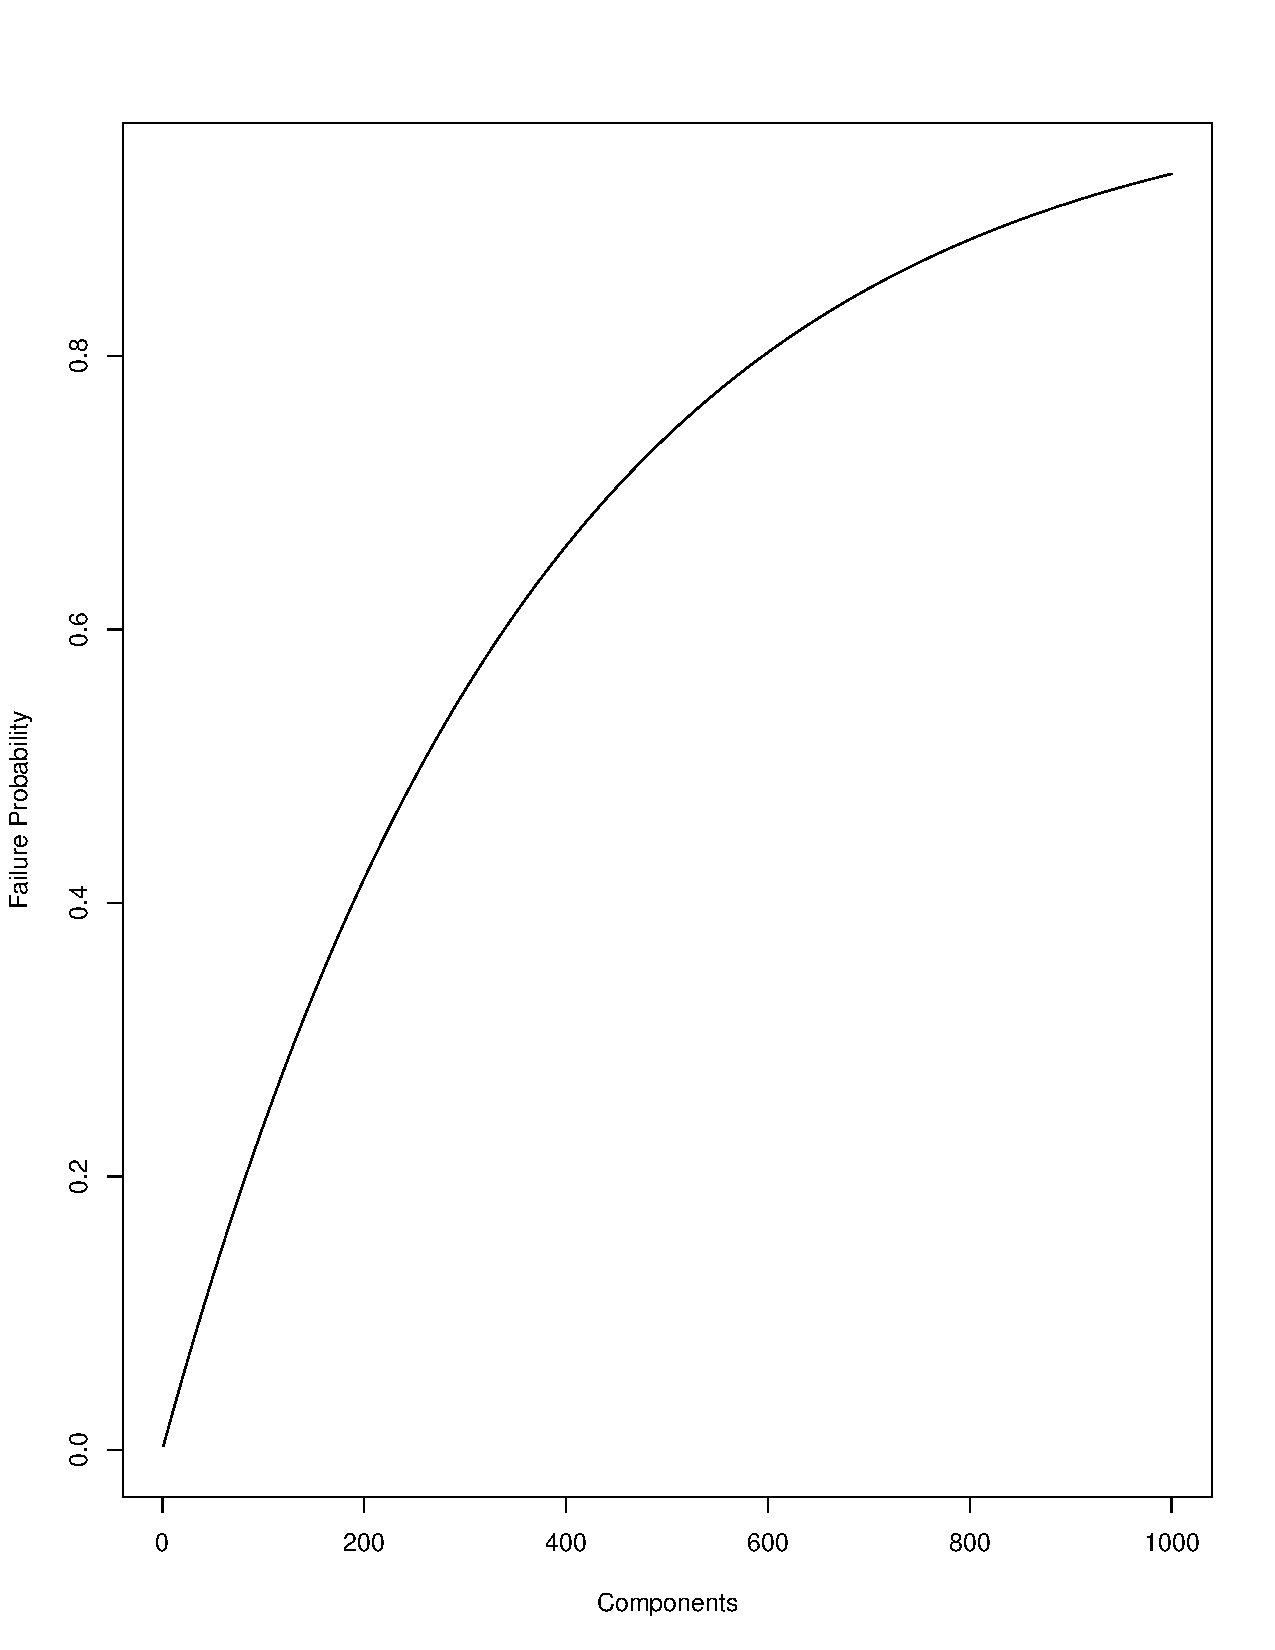
\includegraphics[width=0.8\linewidth]{art/faillure_probability}
\caption[3-sigma probability of failure]{\footnotesize 
	The probability of failure as a function of components under the 3-sigma standard.}
\label{fig:3_sigma_failure_proability}
\end{minipage}\hfill
\begin{minipage}{0.45\textwidth}
\centering
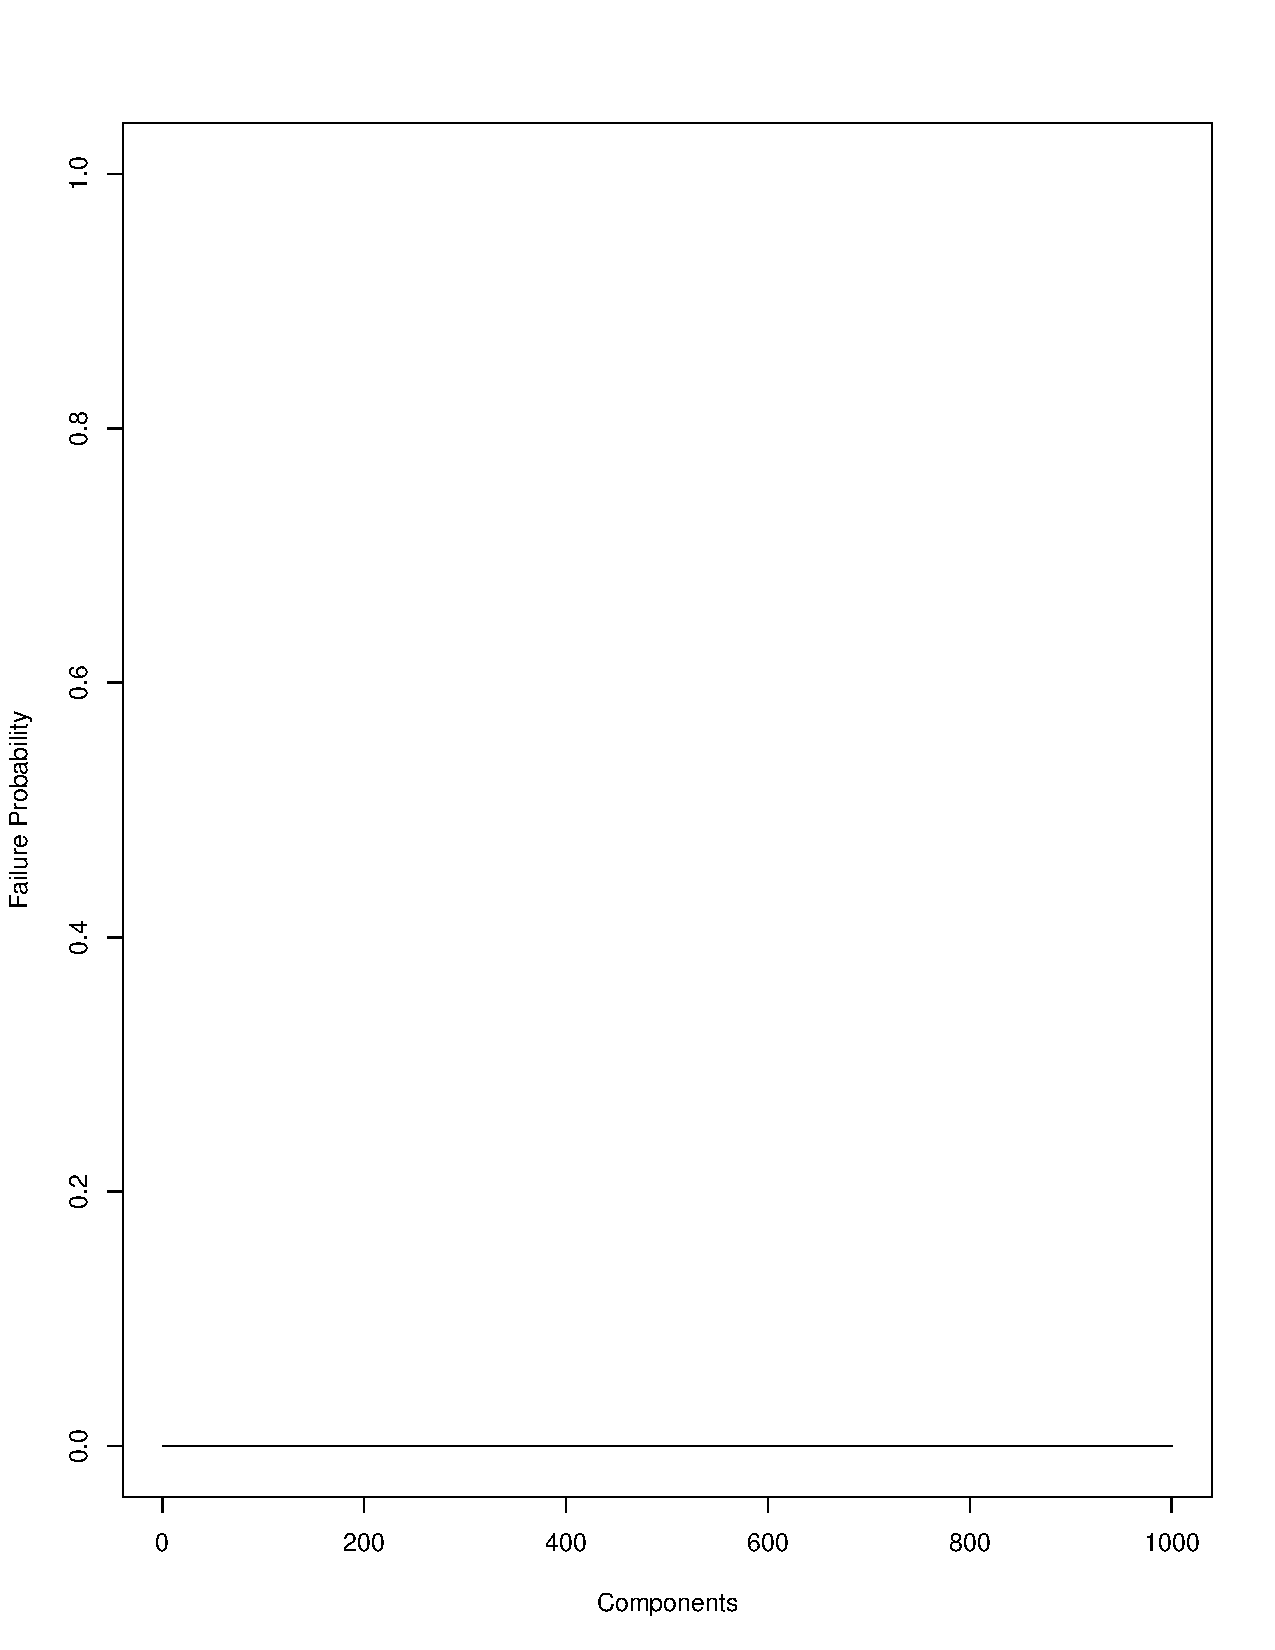
\includegraphics[width=0.8\linewidth]{art/6-sigma_failure_probability}
\caption[6-sigma probability of failure]{\footnotesize 
	The probability of failure as a function of components under the 6-sigma standard.}
\label{fig:6_sigma_failure_proability}
\end{minipage}
\end{figure}

According to \cite{montgomery_introduction_2007}, the 6-sigma methodology has gained more success than it predecessors:
\begin{quote}
The reason for the success of six-sigma in organizations outside the traditional manufacturing sphere is that variability is everywhere, and where there is variability, there is an opportunity to improve business results. 
\end{quote}



\subsection{Lean Systems}
Quoting \cite{wikipedia_lean_2015} (my own emphasis in bold):
\begin{quote}
Essentially, lean is centered on making obvious what \textbf{adds value} by \textbf{reducing everything else}. Lean manufacturing is a management philosophy derived mostly from the Toyota Production System (TPS) (hence the term Toyotism is also prevalent) and identified as ``lean'' only in the 1990s.
\end{quote}

\subsection{Design for Six-Sigma (DFSS)}
\label{sec:dfss}

Quoting \cite{wikipedia_design_2015} (my own emphasis in bold):
\begin{quote}
It is based on the use of \textbf{statistical tools} like linear regression and enables empirical research similar to that performed in other fields, such as social science. While the tools and order used in Six Sigma require a process to be in place and functioning, DFSS has the objective of \textbf{determining the needs of customers} and the business, and driving those needs into the product solution so created. DFSS is relevant for relatively simple items / systems. It is used for product or process design in contrast with process improvement.
\end{quote}




\subsection{Quality Systems and Standards}
The first quality standard was issued by the International Standards Organization (ISO) in $1987$.\marginnote{ISO9000}
Current quality standards are known as the \emph{ISO9000 series}. These include:
\begin{description}
\item [ISO9000:2000] Quality Management System-Fundamentals and Vocabulary.
\item [ISO9001:2000] Quality Management System-Requirements.
\item [ISO9004:2000] Quality Management System-Guidelines for Performance Improvement.
\end{description}
In Israel, it is the Standards Institute of Israel\footnote{\url{https://portal.sii.org.il/heb/qualityauth/certificationtypes/qualitylinks/iso9001/}} that may give ISO9000 (like any ISO) certifications upon inspecting the candidate organization.
As emphasized by \citet[p.24]{montgomery_introduction_2007}, ISO9000 is a set of rules and best practices, mostly oriented at \emph{knowledge management}. 
It may help to \emph{preserve} quality, but it does not, nor does it aim to, \emph{improve} quality.
As such, it will not be the focus of our course, which will focus on \emph{statistical tools}.


\begin{extra}

[TODO: Just-in-Time, Poka-Yoke]

\end{extra}




\section{DMAIC}
There are many names for the process of quantitative re-evaluations of performance against a given target: \emph{data driven decision making} (DDD), \emph{Shewart cycle}, etc.
We will focus on one such framework, illustrated in Figure~\ref{fig:DMAIC} known as DMAIC: Define, Measure, Analyze, Improve, Control.


\begin{figure}[t]
\centering
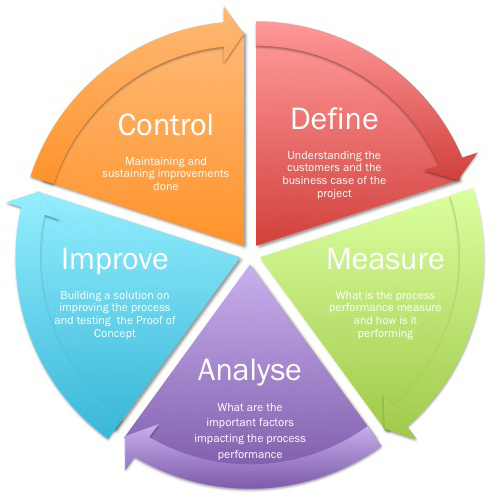
\includegraphics[width=0.6\linewidth]{art/Sigma_detail}
\caption[DMAIC]{The DMAIC cycle. \newline
\url{http://www.sapartners.com/sigma-academy/}}
\label{fig:DMAIC}
\end{figure}

Here are some general observations on DMAIC:
\begin{enumerate}
\item It is aimed at promoting improvement and creative thinking.
\item It is not part of the six-sigma methodology, but will typically take part in its implementation.
\end{enumerate}

What do the stages of DMAIC mean \footnote{\url{http://asq.org/learn-about-quality/six-sigma/overview/dmaic.html}}?
\begin{description}
\item [Define] the problem, improvement activity, opportunity for improvement, the project goals, and customer (internal and external) requirements.
\item [Measure] process performance.
\item [Analyze] the process to determine root causes of variation, poor performance (defects).
\item [Improve] process performance by addressing and eliminating the root causes.
\item [Control] the improved process and future process performance.
\end{description}

In the following chapter we give a set of statistical tools required for \emph{measuring},\emph{analyzing} and \emph{controlling} a process.




\section{Bibliographic Notes}
[TODO] 
\chapter{Exploratory Data Analysis}
\chaptermark{EDA}
\label{sec:exploratory}


In this chapter, we give a short review of methods for \emph{exploratory data analysis} (EDA), \aka \emph{descriptive statistics}.\marginnote{Descriptive Statistics}
Recall that our goal is an assumptions-free description of our data. 
EDA thus consist of computing interpretable summaries of the data, called \emph{summary statistics}, and visualizations. 


\section{Summary Statistics}
\label{sec:summary_statistics}

We now distinguish between summary statistics that apply to attributes, categorical by definition, and variables, continuous by definition. 


\subsection{Summarizing Categorical Data}

\subsubsection{Univariate}
Summarizing a vector of categorical data can naturally be done by tabulating it, i.e., computing the frequency and relative frequency of each category.
Clearly averages, medians, and the likes are incomputable, since categorical data has no ordering, nor does it admit simple operations such as summation.

\begin{extra}
Variability of categorical data can clearly not be measured by its variance, since it does not admit a summation operation.
It is, however, possible to define different measures of variability that do apply.
The \emph{entropy} is such an example.\marginnote{Entropy}
\end{extra}


\subsubsection{Bivariate}
Generalizing the univariate case to bivariate, or multivariate, one can keep tabulating. I.e., compute the frequency, and relative frequency, of combinations of categories.



\subsection{Summarizing  Continuous Data}
Continuous variables admit many more mathematical manipulations than categorical attributes. 


\subsubsection{Univariate}

We start by presenting the most natural summaries of the data. Without going into the formal definition, we refer to them as \emph{summary of location}.\marginnote{Location Summaries}
These include:

\begin{definition}[The Mean]
The \emph{mean}, or \emph{average}, is defined as 
\begin{align}
	\bar{x}:= \frac{1}{n}\sum_{i=1}^{n} x_i
\end{align}
\end{definition}

\begin{definition}[The Median]
The median is the observation that is smaller than half of the sample and larger than half of the sample.
\end{definition}

\begin{definition}[$\alpha$-Trimmed Mean]
The $\alpha$-trimmed mean is the average of the observations left after ignoring the largest and the smallest $(100\alpha) \%$ of them.
\end{definition}
The \naive average is the $0$-trimmed mean, and the median is the $0.5$-trimmed mean.

From summaries of location, we move to summaries of \emph{scale}. \marginnote{Summary of Scale}

\begin{definition}[The Standard Deviation]
\begin{align}
	s(x):= \sqrt{\frac{1}{n-1} \sum_{i=1}^{n} (x_i-\bar{x})^2}
\end{align}
\end{definition}

For the following, we require the definition of the sample quantiles, themselves \textbf{not} a scale summary.

\begin{definition}[$\alpha$ Quantile]
The $\alpha$-quantile of the sample is the observation that is larger than $(100\alpha)\%$, and smaller then  $(100(1-\alpha))\%$ of the sample. 
\end{definition}
The empirical maximum and minimum are then $x_{1.0}$ and $x_{0.0}$, respectively.


\begin{definition}[The Range]
\begin{align}
	Range(x):= \max_i\set{x_i}-\min_i\set{x_i}= x_{1.0}-x_{0.0}
\end{align}
\end{definition}

\begin{definition}[The Inter Quantile Range- IQR]
\label{def:iqr}
\begin{align}
	IQR(x):= x_{0.75}-x_{0.25}
\end{align}
\end{definition}



\begin{definition}[The Median Absolute Deviation- MAD]
\label{def:mad}
\begin{align}
	MAD(x):= \set{|x_i-x_{0.5}|}_{0.5} 
\end{align}
\end{definition}
Note that the MAD may be sometimes scaled by $1.4826$, so that it estimates $\sigma$. Such is the behaviour of the \R function \rcode{mad()}. 


After summaries of scale, we move to summaries of \emph{skewness}, or \emph{asymmetry}.

\begin{definition}[Yule Skewness Measure]
\begin{align}
	YULE(x):= \frac{\frac{1}{2} (x_{0.75}+x_{0.25})-x_{0.5}}{IQR(x)}
\end{align}
\end{definition}

 


\subsubsection{Bivariate}
From univariate data $x$, we move to bivariate $x,y$.
Clearly we can apply univariate summaries component-wise. 
We want, however, to summarize the \emph{joint} behaviour of the data. 
For this purpose, we assume that data comes in pairs, implying that $x$ and $y$ are of same length.


\begin{definition}[Covariance]
The sample covariance, or \emph{empirical} covariance is defined as
\begin{align}
	Cov(x,y):= \frac{\sum_{i=1}^{n} (x_i-\bar{x})(y_i-\bar{y})}{n-1}
\end{align}
\end{definition}



\begin{definition}[Pearson's Correlation Coefficient]
\emph{Pearson’s Correlation Coefficient}, or \emph{Pearson's Moment Product Correlation Coefficient}, is defined as
\begin{align}
	r(x,y):= \frac{(n-1) Cov(x,y)}{S(x) S(y)}= \frac{\sum_{i=1}^{n} (x_i-\bar{x})(y_i-\bar{y})}{S(x) S(y)}
\end{align}
\end{definition}
We can dwell into the meaning and intuition underlying Pearson's correlation coefficient, but we will not. 
The curious reader is reffered to \cite{rodgers_thirteen_1988}.

The next measure of association captures a more general association.
\begin{definition}[Spearman's Correlation Coefficient]
Spearman's correlation coefficient is merely Pearson's correlation coefficient computed on the \emph{ranks} of $x$ and $y$. 
\end{definition}

We conclude by noting that \emph{regression coefficients} are also a measure of association. 





\subsubsection{Multivariate Data}
Multivariate data, both continuous (variables), and discrete (attributes), admits a vast realm of method for summary and visualization.
Clearly, associations between several variables can be very complicated so that the more we try to summarize, the more information we give up. On the other hand, and unlike the univariate and bivariate case, our minds will need some type of simplification since they cannot grasp the raw data (did you ever try to imagine how $\mathbb{R}^4$ looks like?).
As usual, we emphasize that our purpose is to summarize the joint association in the data. 
For component-wise summaries, we can always apply the univariate summaries one variable at a time. 

By far the most popular measures of joint association are the covariance matrix and correlation matrix.

\begin{definition}[Covariance Matrix]
For multivariate data consisting of $x_1,\dots,x_j,\dots,x_p$ vectors, each with $n$ entries: $x_{j,1},\dots,x_{j,n}$, we define the (sample) covariance matrix to be a $p\times p$ matrix whose elements are the (sample) covariances between corresponding vectors:
\begin{align}
	\hat{\Sigma}_{k,l}:= Cov(x_k, x_l).
\end{align}
\end{definition}


\begin{extra}[Sample Covariance Matrix]
The matrix $\hat{\Sigma}$ has many useful properties. 
The curious reader is referred to \cite{petersen_matrix_2006}, and references therein, for more details.
\end{extra}

\begin{definition}[Correlation Matrix]
For multivariate data consisting of $x_1,\dots,x_j,\dots,x_p$ vectors, each with $n$ entries: $x_{j,1},\dots,x_{j,n}$, we define the (sample) correlation matrix to be a $p\times p$ matrix whose elements are the (Pearson) correlations between corresponding vectors:
\begin{align}
	\hat{R}_{k,l}:= r(x_k, x_l)
\end{align}
\end{definition}


\begin{extra}[Multivariate Data Analysis]
Multivariate analysis is an important, and very actively studied field in statistics and machine learning.
A non-comprehensive list of methods that belong to this realm include 
Principal Component Analysis (PCA),\marginnote{PCA, SVD,ICA}
Singular Value Decomposition (SVD), 
Factor Analysis (FA), 
Independent Component Analysis (ICA),
Dimensionality Reduction, 
Manifold Learning, 
Self Organizing Maps, 
etc.
Ask me for reference books or courses if this topic interests you.
\end{extra}

\afterpage{\clearpage}


\section{Visualization}
\label{sec:visualizations}

\subsection{Visualizing Categorical Data}



\subsubsection{Univariate}
Much like computing summaries, there is not much to be said about visualizing univariate categorical variables. 
The most natural, and perhaps only visualization, is the \emph{bar plot}, illustrated in Figure~\ref{fig:barplot}.

\begin{remark}[Pie Chart]
About those pie charts. 
There is really no reason to use them. Ever\footnote{\url{http://www.businessinsider.com/pie-charts-are-the-worst-2013-6}.}.
\end{remark}



\begin{figure}[h]
\centering
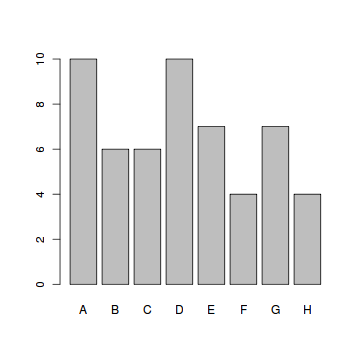
\includegraphics[height=0.3\textheight]{art/categorical-data1x}
\caption[Bar Plot]{The Bar-Plot. \newline
\url{http://www.r-tutor.com/elementary-statistics/qualitative-data/bar-graph}}
\label{fig:barplot}
\end{figure}



\subsubsection{Bivariate}
Visualizing a two-way cross-table can be done using an extension of the bar-plot.
Several extensions exist. By far, the most informative and recommended figure, in this author's view, is the \emph{mosaic plot}, illustrated in Figure~\ref{fig:mosaic}. \marginnote{Mosaic Plot}

\begin{figure}[h]
\centering
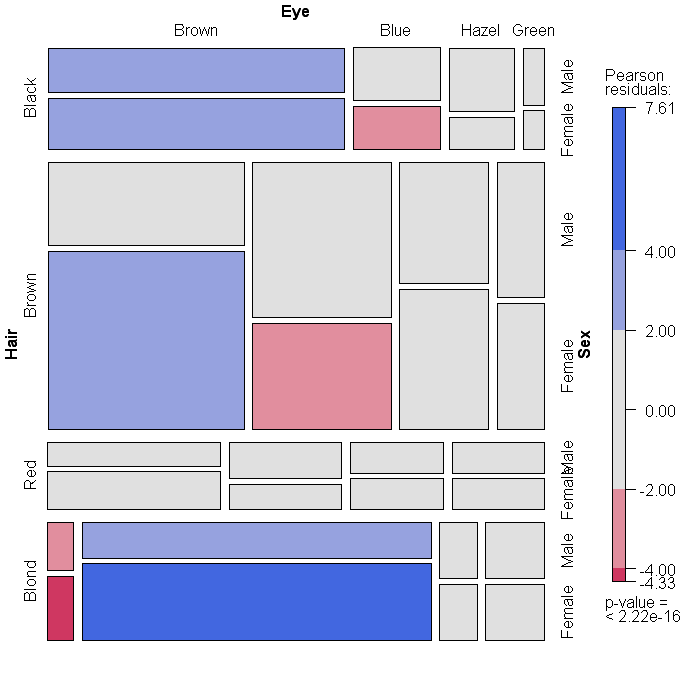
\includegraphics[height=0.3\textheight]{art/mosaic1}
\caption[Mosaic Plot]{Mosaic Plot. \newline
\url{http://www.statmethods.net/advgraphs/mosaic.html}}
\label{fig:mosaic}
\end{figure}







\afterpage{\clearpage}


\subsection{Visualizing Continuous Data}




\subsubsection{Univariate}
Visualization of univariate continuous vectors can present the raw data, or it distribution (i.e.- discarding the indexes).
The most basic visualizations are the \emph{dotchart}, \emph{histogram}, \emph{boxplot}, \emph{stem-and-leaf plot}. 
These are illustrated in figures \ref{fig:dot_plot}, \ref{fig:histogram_eruptions}, \ref{fig:boxplot}, \ref{fig:stem_and_leaf} respectively. 


 
\begin{figure}[h]
\centering
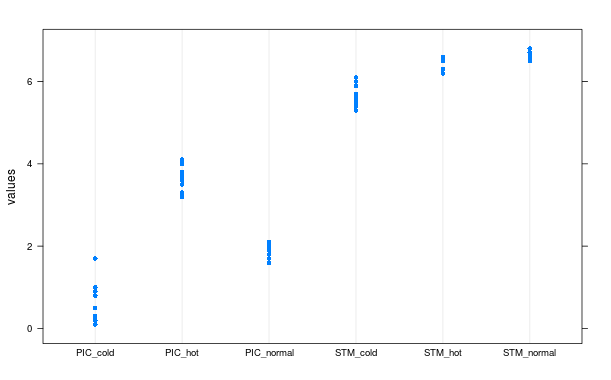
\includegraphics[height=0.3\textheight]{art/lmCm0}
\caption[Dot Plot]{Dot Plot. \newline \url{http://stackoverflow.com/questions/15109822/r-creating-scatter-plot-from-data-frame}}
\label{fig:dot_plot}
\end{figure}



\begin{figure}[h]
\centering
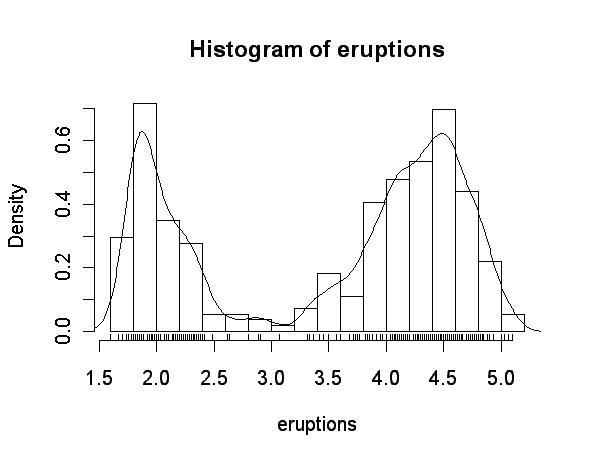
\includegraphics[height=0.3\textheight]{art/histogram_eruptions}
\caption[Histogram]{Histogram. 
Notice the ticks on the x axis. These are the raw data points. Make sure you always add them, with the \rcode{rug()} \R command. 
\newline \url{http://compbio.pbworks.com/w/page/16252882/Basic}}
\label{fig:histogram_eruptions}
\end{figure}

\begin{figure}[h]
\centering
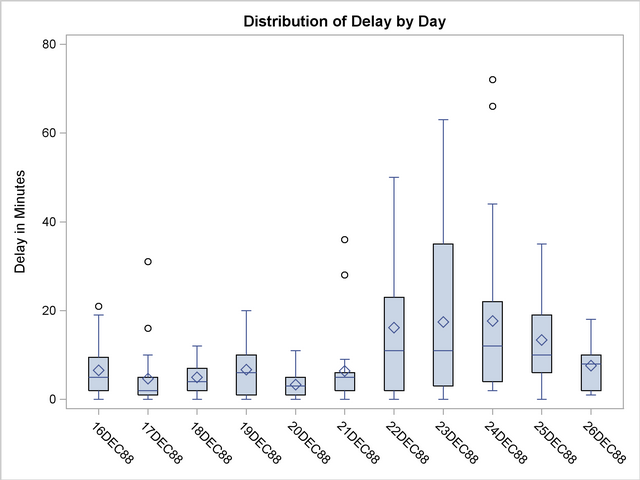
\includegraphics[height=0.3\textheight]{art/ex6aout}
\caption[BoxPlot]{Boxplot. \newline \url{http://support.sas.com/documentation/cdl/en/statug/63033/HTML/default/viewer.htm}}
\label{fig:boxplot}
\end{figure}



\begin{figure}[h]
\centering
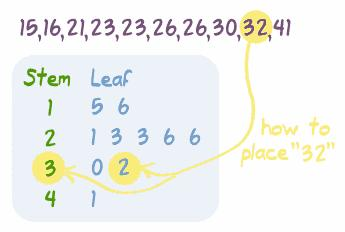
\includegraphics[height=0.3\textheight]{art/stem_and_leaf}
\caption[Stem and Leaf Pot]{Stem-and-leaf plot. \newline
\url{https://www.mathsisfun.com/data/stem-leaf-plots.html}}
\label{fig:stem_and_leaf}
\end{figure}




\subsubsection{Bivariate}
The simultaneous visualization of two continuous variables, can naturally be done with a \emph{scatter plot}.
More sophisticated visualization, which generalizes the histogram into two dimensions, is the \emph{hexbin plot}.  
These are illustrated in figures \ref{fig:scatterplot}, and \ref{fig:hexbin}, respectively. 


\begin{figure}[h]
\centering
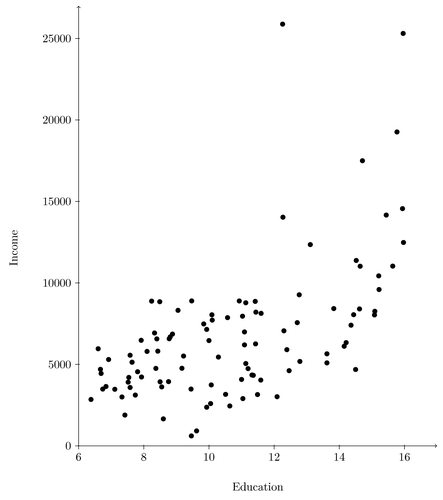
\includegraphics[height=0.3\textheight]{art/scatterplot}
\caption[Scatter Plot]{Scatter Plot. \newline 
\url{http://texample.net/tikz/examples/scatterplot/}}
\label{fig:scatterplot}
\end{figure}





\begin{figure}[h]
\centering
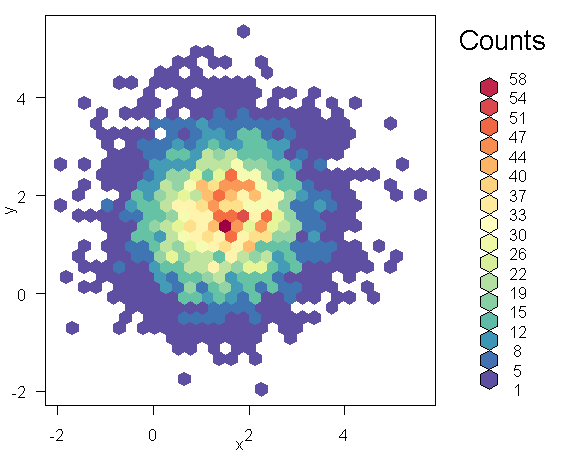
\includegraphics[height=0.3\textheight]{art/hexbin2}
\caption[HexBin Plot]{HexBin plot (a 2D histogram).
\newline \url{http://www.r-bloggers.com/5-ways-to-do-2d-histograms-in-r/}}
\label{fig:hexbin}
\end{figure}






\subsubsection{Multivariate Data}
Since we cannot possibly visualize data in more than $3$-dimensions, and we clearly prefer data in $1$ or $2$ dimensions, the visualization of multivariate data will typically consist of summarizing the data into $1D$ or $2D$, and then applying the above mentioned visualization techniques.

An important exception is due to the observation that a computer image, is essentially a matrix. 
We can thus visualize matrices, with a simple image, and in particular, covariance and correlation matrices, as illustrated in Figure~\ref{fig:covariance_image}.

A second exception is when the data has both continous variables and discrete attributes. 
Endlessly many combinations are then possible.
The author strongly recommends to visit Hans Rosling's \emph{Gap Minder} at \url{http://www.gapminder.org/world} for an excellent interactive visualization. \marginnote{Gap Minder}


\begin{figure}[h]
\centering
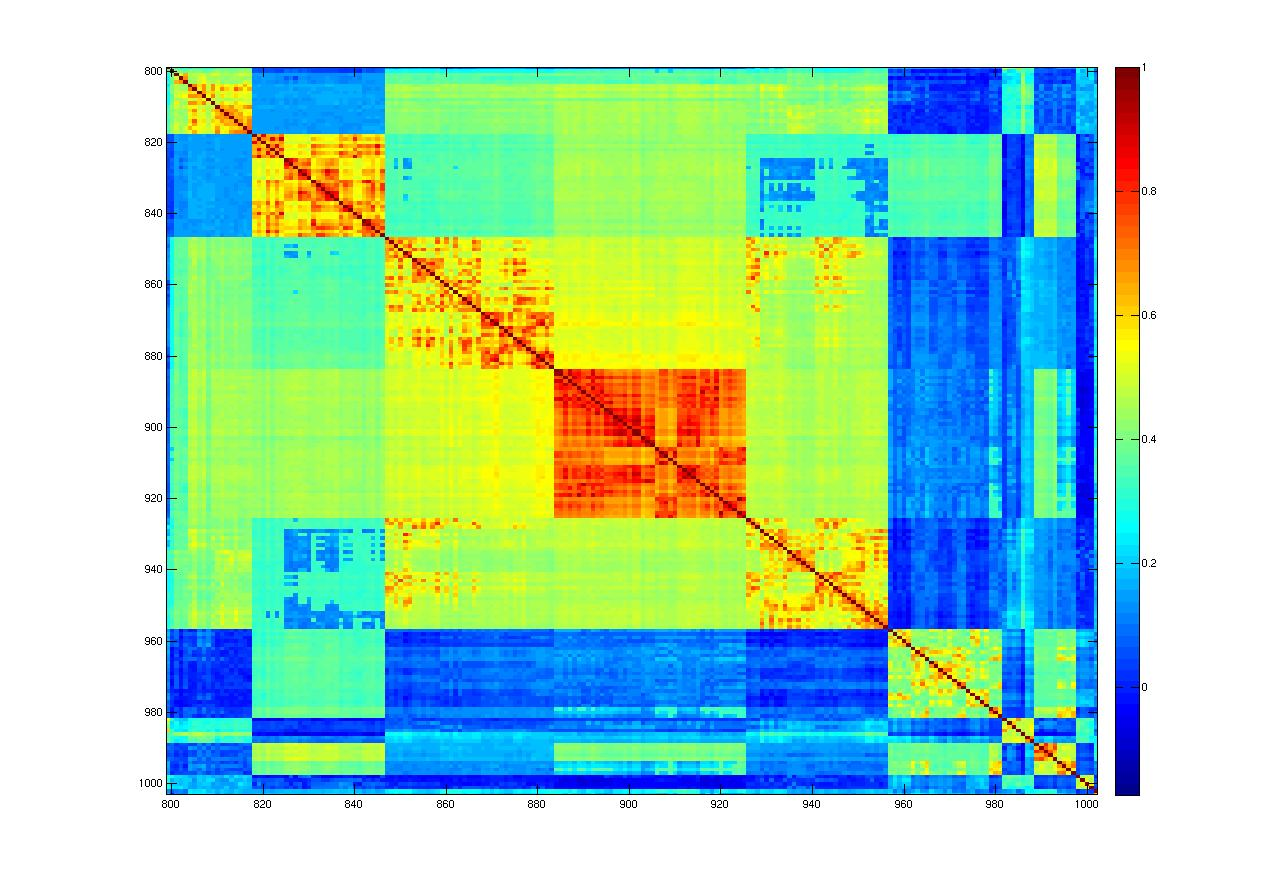
\includegraphics[height=0.3\textheight]{art/covarianceSupervised}
\caption[Covariance Matrix]{Image of covariance matrix. \newline
\url{http://cs.brown.edu/courses/csci1950-g/results/final/sghosh/}}
\label{fig:covariance_image}
\end{figure}




\subsection{On-Line Visualization}
For the purpose of quality control, we may often want an \emph{on-line} visualization, and not \emph{off-line}, as the ones previously discussed.
This is the purpose of \emph{dashboards}, illustrated in Figure~\ref{fig:dashboard}.\marginnote{Dashboard}

\begin{figure}[h]
\centering
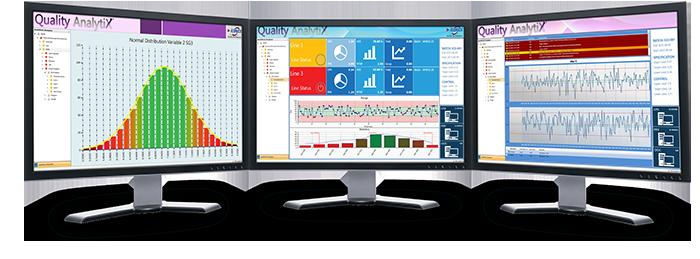
\includegraphics[height=0.3\textheight, width=0.9\linewidth]{art/dashboard}
\caption[Dashboard]{Dashboard. \newline
\url{http://www.iconics.com/Home/Products/AnalytiX/Quality-AnalytiX.aspx}}
\label{fig:dashboard}
\end{figure}

\afterpage{\clearpage}

\chapter{Statistical Inference} 
\chaptermark{Inference}
\label{sec:inference}

The idea of extrapolating knowledge from a \emph{sample} to a population is known as \emph{statistical inference}.
It encompasses the ideas of \emph{parameter estimation}, \emph{confidence intervals}, and \emph{hypothesis testing}.
We will assume the reader is familiar with these, but recall some required terminology.
The QC and SPC terminology are not always consistent with statisticians' terminology. When new names are given to old ideas, we will emphasize this in the text.

\begin{description}
\item [Null/Alternative Hypothesis] Some statement about the world we wish to test with data. The frequentist argument follows a Popperian philosophy\DIFaddbegin \footnote{\DIFadd{Following Karl Popper's philosophy of science, we can never know that something is true, we can only know when it is not true. Popper philosophy was motivated by the fact that no one suspected Isaac Newton's mechanics to be wrong, until relativity theory was proposed by Einstein.}}\DIFaddend : to show the alternative hypothesis is true, we will show that the null hypothesis is not true. 
In the context of quality control, the null hypothesis will be the process is \emph{in statistical control}, while the alternative will be that it is \emph{out of control}.\marginnote{In Control}
\item [Statistical Test] The procedure of inferring from data on the truthfulness of the alternative hypothesis.
\item [Assumptions] As the name suggests, these are assumptions. We stress that unlike hypothesis, assumptions are not being tested in a statistical test. 
\item [Test Statistic] The function of the data to be computed for the purpose of inference. As such, it is a random variable. 
\item [Null/Alternative Distribution] The distribution of the test statistic under the null/alternative hypothesis.
\item [Type I/II error] See Figure~\ref{fig:confusion_table}.
\item [False/True Positive/Negative] See Figure~\ref{fig:confusion_table}.
\item [Rejection Region] The collection of event that will lead us to reject the null hypothesis, and believe in the alternative hypothesis.
\item [p-value] A.k.a. \emph{observed significance}. The null probability of the observed (or ``more extreme'') event.
\item [Significance Level] A.k.a. $\alpha$. The probability of a false positive.
\item [Power] The probability of a true positive.
\item [i.i.d.] ``Independent and identically distributed'' (i.i.d.) is an assumption made on the sampling distribution, meaning that samples are statistically independent, and all originating from the same distribution.

\end{description}

\begin{figure}
\centering
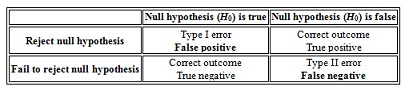
\includegraphics[width=0.8\linewidth]{art/Beware-of-False-Positives-Chart-1}
\caption[Confusion Table]{Type I/II error confusion table. \newline \url{https://infocus.emc.com/william_schmarzo/beware-of-false-positives/}}
\label{fig:confusion_table}
\end{figure}


The following sections of this chapter present particular statistical inference methods we will be using in the following chapters.


\section{Goodness of Fit (GOF)}
\sectionmark{GOF}

Goodness of fit (GOF) deals with the inference on the sampling distribution, a.k.a., the generative process.
It can be approached via rigorous hypothesis testing, or by visualizations.

\subsection{QQplot and QQnorm}
\label{sec:qqplot}

The fundamental idea of the \emph{quantile-quantile plot} (QQplot) is to compare the empirical quantiles in the sample, to the theoretical quantiles implied by the assumed distribution. If the theory and observations agree, we conclude our assumptions are plausible. 
For the particular case of testing the normality of the data, the corresponding QQplot is known as a \emph{QQnorm plot}.

Figure~\ref{fig:qqnorm_normal} illustrates a QQnorm plot of normal distributed data, while Figure~\ref{fig:qqnorm_non_normal} is the same for non-normal data.


\begin{figure}[h]
\centering
\begin{minipage}{0.45\textwidth}
\centering
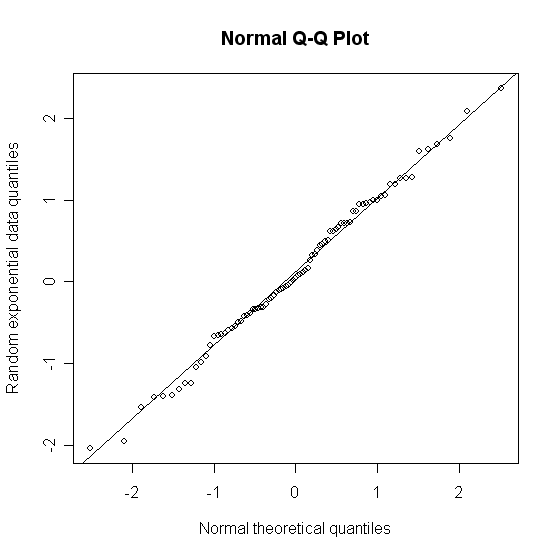
\includegraphics[height=0.3\textheight]{art/Qqnorm}
\caption[QQnorm- Gaussian]{A QQplot of Gaussian distributed data.}
\label{fig:qqnorm_normal}
\end{minipage}\hfill
\begin{minipage}{0.45\textwidth}
\centering
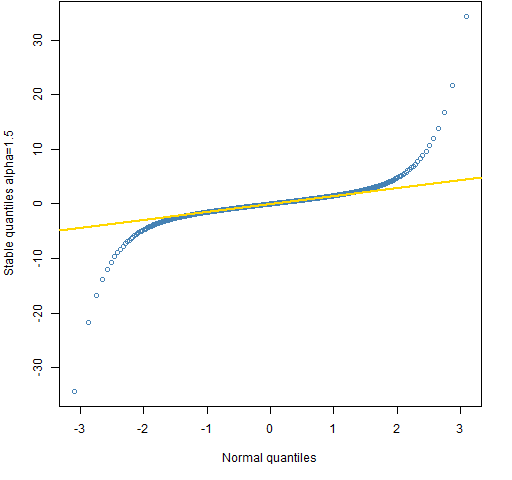
\includegraphics[height=0.3\textheight]{art/stab15qqnorm}
\caption[QQnorm- non Gaussian]{A QQnorm plot of non Gaussian distributed data.}
\label{fig:qqnorm_non_normal}
\end{minipage}
\end{figure}




\subsection{Chi-Square GOF Test}
The Chi-Square GOF test (not to be confused with the Chi-Square independence test), tests a hypothesis on the sampling distribution of discrete (attributes) data. 
Note that it is very general, since all continuous variables may be discretized, simply by binning.

\begin{definition}[Chi-Square GOF Test]
Assume an i.i.d. sample $x_1,\dots,x_n$. 
The Chi-Square GOF is a tests $H_0: \x_i \sim \dist$ versus $H_1: \x_i \not\sim \dist$.
$P$ is assumed to be discrete with $K$ categories and $p_k:= \dist(\x_i \in k)$.
The test statistic, $X^2$, is defined as
\begin{align}
	X^2:= \sum_{k=1}^{K}\frac{(obs_k-exp_k)^2}{exp_k}, 
\end{align}
where $obs_k:= \#\set{x_i \in k}$, and $exp_k:= p_k n$.
The approximate null distribution of $X^2$ is $\chi^2_{K-1}$.
\end{definition} 



\subsection{Kolmogorov–Smirnov GOF Test}
The Kolmogorov-Smirnof GOF test, tests a hypothesis on the sampling distribution of continuous (variable) data. 

\begin{definition}[Kolmogorov–Smirnov GOF Test]
Assume an i.i.d. sample $x_1,\dots,x_n$. 
The Chi-Square GOF is a tests $H_0: \x_i \sim \dist$ versus $H_1: \x_i \not\sim \dist$.
$P$ is assumed to be continuous.
The test statistic, $D$, is depicted in Figure~\ref{fig:ks_test}.
The null distribution of $D$ is the \emph{Kolmogorov distribution} obtained from tables.\marginnote{Kolmogorov Distribution}

\begin{figure}
\centering
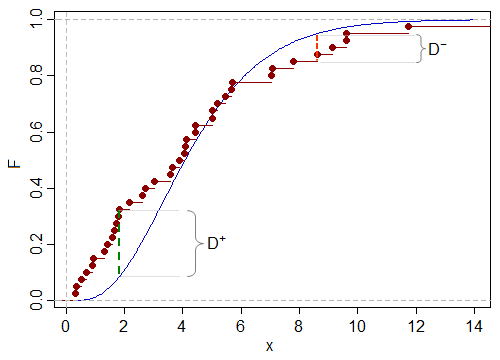
\includegraphics[height=0.3\textheight]{art/Kgn0O}
\caption[Kolmogorov-Smirnov Test]{Kolmogorov-Smirnov Test. The $D$ statistic is $D_+$ in the figure.}
\label{fig:ks_test}
\end{figure}

\end{definition} 






\begin{extra}[GOF tests]
There are endlessly many more GOF tests, such as Anderson-Darling, Jarque–Bera, Shapiro–Wilk, Kuiper's test, etc.
Wikipedia is a good place for further reading.
\end{extra}

\chapter{System Capability Analysis}
\chaptermark{Capability}
\label{sec:capability_analysis}

In a \emph{system capability analysis}, we essentially use statistical tools to measure the variability in a production process.
This analysis can answer questions that are raised at the measuring, analyzing, and improving stages of the DMAIC cycle. 
The methods we will discus compare between the processes variability and its specifications. 

We naturally want production processes that adhere to specifications, and want to quantify the level of adherence.
The quantification is performed by comparing the variability in a CTQ to the specification.
In this chapter we assume the process’s capability is fixed over time. 
In Chapter~\ref{sec:advanced_capability_analysis} we revisit the same problems, when allowing the process’s capability to vary over time. 

The particular setup discussed in this chapter is also known as \emph{product specification}.\marginnote{Product Specification}
When we use the actual time, and ordering of data samples, as in a control chart, we will no longer regard it as product specification but rather as a bona-fide capability analysis. This is the subject of Chapter~\ref{sec:advanced_capability_analysis}.



 
 
 
Because capability analysis, or product specification, is essentially the study of the CTQ's distribution, it can be approached with the aforementioned statistical tools such as univariate summary statistics and visualizations presented in Sections~\ref{sec:summary_statistics} and \ref{sec:visualizations}.
To test a particular hypothesis on the distribution of the CTQ, we may call upon the inference tools from Chapter~\ref{sec:inference}.




\section{Process Capacity Indexes}
\sectionmark{PCRs}

Classical statistical devices do not incorporate the designed process's capabilities.
\emph{Process capability ratios} (PCR), or \emph{process capability indexes}, are merely population parameters that also depend on specifications.\marginnote{Process Capability Index}
The first, and most basic PCR is the $\cp$ of a particular CTQ.

\begin{definition}[$\cp$]
\begin{align}
\label{eq:cp}
	C_p:= \frac{USL-LSL}{6 \sigma}, 
\end{align}
where $\sigma$ is the standard deviation of the CTQ.
Eq.(\ref{eq:cp}) readily offers an interpretation of the $\cp$: it measures how accurate is our process compared to a 3-sigma process: $\cp=1$ for 3-sigma, $\cp=2$ for 6-sigma, etc.
\end{definition}
Clearly $\cp$ is a process parameter, that needs to be estimated.
\begin{definition}[$\cpHat$]
\begin{align}
	\cpHat:= \frac{USL-LSL}{6 \hat{\sigma}}, 
\end{align}
where $\hat{\sigma}$ is some estimate of the standard deviation of the CTQ.
\end{definition}
The most natural $\hat{\sigma}$ is the sample standard deviation $s$, but we will explore other options in the following.


There is a relation between $C_p$ and the probability of non-conformance. 
To explore this relation we introduce the following notation:
\begin{tcolorbox}
\footnotesize
\textbf{Collecting Notation} \newline
$\targetValue$, the target value. \newline
$\delta:= (USL-LSL)/2$, the specification tolerance. $USL=\targetValue+\delta, LSL=\targetValue-\delta$.  \newline
$\ctqExpect:= \expect{CTQ}$, the expected CTQ. \newline
$\pnc:= 1-P(CTQ \in [LSL,USL])$, the probability of non compliance. 
\end{tcolorbox}

With our new notation Eq.(\ref{eq:cp}) is now $\cp=\frac{\delta}{3 \sigma}$.
Assuming $CTQ \sim \gauss{\mu, \sigma^2}$, and that the process is centred so that $\ctqExpect=\targetValue$, then $\cp$ is related to $\pnc$ via
\begin{align}
\label{eq:pc_and_pnc}
	\pnc= 2\, \Phi(-3 \cp)
\end{align}
As a sanity check, we check this relation for a 3-sigma process.
A 3-sigma process implies that $\cp=1$, and Eq.(\ref{eq:pc_and_pnc}) returns $\pnc=0.0027$, as we have already seen in the introduction (Section~\ref{sec:six_sigma}).

\cite{montgomery_introduction_2007} recommends the following $\cp$ values:

\begin{tabular}{|c|c|c|}
\hline  & $\cp$ Value & Implied ppm \\ 
\hline \hline Existing processes
 & 1.33
 & 66 \\ 
\hline New processes
 & 1.50
 & 6.8 \\ 
\hline Safety, strength, or critical
parameter, existing process
 & 1.50
 & 6.8 \\ 
\hline Safety, strength, or critical
parameter, new process
 & 1.67
 & 0.5 \\ 
\hline Six Sigma quality process & 2.00 &  0.002 \\ 
\hline 
\end{tabular} 

\bigskip

To derive Eq.(\ref{eq:pc_and_pnc}), and thus the ppm column in the table, we had to call upon several assumptions.
Namely:
\begin{enumerate}
\item The CTQ has a normal distribution.
\item The process is centred, i.e. $\ctqExpect=\targetValue$.
\end{enumerate}








\subsection{Non-Conformance for a Non-Gaussian CTQ}
The first assumption we will now relax is the Gaussianity of $CTQ$. 
We start by checking what is the non compliance rate, if we were completely wrong about the distribution of the CTQ. 
Chebyshev's inequality provides a universal bound on $\pnc$.


\begin{theorem}[Chebyshev's inequality]
For any random variable $\x$, with $\mu:=\expect{\x}$, and $\sigma^2:=\expect{(\x-\mu)^2}$, then
\begin{align}
	P(|\x-\mu| \geq k\sigma) \leq \frac{1}{k^2}.
\end{align}
\end{theorem}
If $\cp=1$  then $\delta=3\sigma$. Plugging $k=3$ in the inequality returns $\pnc<0.11$.
This means that a 3-sigma process, assumingly with $2,700 ppm$, may actually have $111,111 ppm$, if we were very very wrong about the Gaussianity assumption.



The moral of the story is that by assuming the correct distribution of the CTQ, we may save a lot of resources. 
We can assume normality, as we typically do, but there are other alternatives:
\begin{enumerate}
\item Transformations: it is quite possible that the CTQ is not Gaussian in its original scale, but it is Gaussian in a different scale. You should always inspect a QQnorm (Sec. \ref{sec:qqplot}) plot after a $log$ or $sqrt$ transformation.
\item Assume a different distribution: We derived $\pnc(\cp)$ (eq.~\ref{eq:pc_and_pnc}) under a normality assumption, but it may certainly be derived for different distributions. 
\item The denominator of $\cp$ is a range that leaves $0.00135$ probability of the Gaussian tail outside the range. 
When relaxing the normality assumption, $\sigma$ is no longer related to the tail probability as it was before. We may still, however, directly plug $CTQ_{0.00135}$ and $CTQ_{1-0.00135}$ quantiles to get a CPR in the same spirit of the $\cp$. This is known as the $\cpq$ index we now define.
\end{enumerate}

\begin{definition}[$\cpq$]
\begin{align}
	\cpq:= \frac{USL-LSL}{CTQ_{1-0.00135}-CTQ_{0.00135}}
\end{align}
\end{definition}






\subsection{Process Capability of a Non-Centred Process}
We will now relax the assumption of $\ctqExpect=\targetValue$.

\begin{definition}[$\cpk$]
\begin{align}
	\cpk:= \min\set{\cpu,\cpl}
\end{align}
where $\cpu:= \frac{USL- \ctqExpect}{3 \sigma}$ and $\cpl:= \frac{\ctqExpect-LSL}{3 \sigma}$.
\end{definition}
For a non-centred process, this definition is more informative on the probability of non-compliance.
Indeed, Eq.(\ref{eq:pc_and_pnc}) will not hold, but we can derive an updated version:
\begin{align}
	 \pnc \approx \Phi(-3 \cpk).
\end{align}
Generally, $\cpk \leq \cp$, with equality holding for centred processes ($\ctqExpect=\targetValue$).
An illustration is given in Figure~\ref{fig:cpk}.


\begin{figure}
\centering
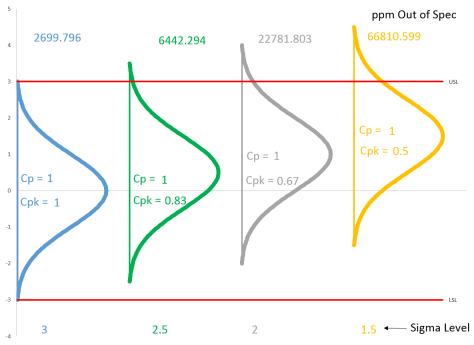
\includegraphics[height=0.3\textheight]{art/Cpk_same_sigma_varying_avg}
\caption[$\cpk$ and $\cp$]{$\cpk$ and $\cp$. \newline
\url{https://www.spcforexcel.com/knowledge/process-capability/interactive-look-process-capability}.}
\label{fig:cpk}
\end{figure}



The $\cpk$ index is motivated by conserving the relation between the index and the non-compliance rate $\pnc$, which is not captured by $\cp$ when the process is not centred. 
Indeed if $\cp$ can be interpreted as ``accuracy compared to a (centred) 3-sigma process'', then $\cpk$ can be interpreted as ``accuracy compared to a (non-centred) 3-sigma process''.
The 3-sigma process is used as a benchmark for historical reasons. 
In practice, it is actually very common to report the sigma-level as a capability index: $\min\set{\frac{USL-\mu}{\sigma},\frac{\mu-LSL}{\sigma}}$, which can be seen as PCR with respect to a 1-sigma process.
Three-sigma would thus be reported as $3$, 6-sigma as $6$, etc.


Another index, known as $\cpm$, or the \emph{Taguchi capability index}, also deals with the non centring but slightly differently. \marginnote{Taguchi Index}
It is motivated by the observation that for $\ctqExpect=\targetValue$, then $\sigma=\sqrt{\expect{(CTQ-\targetValue)^2}}$. This relation does not hold if $\ctqExpect \not=\targetValue$, which leads us to the following definition:
\begin{definition}[$\cpm$]
\begin{align}
		\cpm &:= \frac{USL-LSL}{6 \sqrt{\expect{(CTQ-\targetValue)^2}}} \\
		&= 	\frac{USL-LSL}{6 \sqrt{\sigma^2+(\ctqExpect-\targetValue)^2}} \\ 
		&= \frac{\cp}{\sqrt{1+(\frac{\ctqExpect-\targetValue}{\sigma})^2}}. \label{eq:cpm}
\end{align}
\end{definition}
Eq.(\ref{eq:cpm}) readily shows that just like the $\cpk$, then $\cpm \leq \cp$. 








\subsection{Interval Estimation for Capability Indexes}
Since the various process capability indexes are merely population parameters, we can also construct confidence intervals (CIs) for them, which are very important for small sample sizes, thus point estimates unreliable.
The simplest case is that of $\cp$. Being a monotone transformation of $\sigma$, we can call upon confidence intervals for the variance of a normal population, so that with probability $1-\alpha$:
\begin{align}
\label{eq:ci_for_cp}
	\cp \in \left[ 
		\cpHat \sqrt{\frac{\chi^2_{\alpha/2,n-1}}{n-1}},
		\cpHat \sqrt{\frac{\chi^2_{1-\alpha/2,n-1}}{n-1}}
	\right],
\end{align}
where $\cpHat = \frac{USL-LSL}{6 s}$.
This equation is simply derived from Eq.(\ref{eq:cp_dist}).
Intervals for the other capability indexes, are available in \cite{montgomery_introduction_2007} and references therein. 




\subsection{Testing Hypotheses on Capability}
Consider a supply contract, which requires production to have $\cp>1.5$. 
It may easily be the case, that $\cp>1.5$, even if $\cpHat<1.5$, especially if the sample size is small.
It thus makes a lot of sense, to design hypothesis tests on process capabilities. 
We observe that for an i.i.d. sample from a Gaussian population, where $\cpHat$ is estimated with $s$, then
\begin{align}
\label{eq:cp_dist}
	(n-1) \left( \frac{\cp}{\cpHat} \right)^2  \sim \chi^2_{n-1},
\end{align} 
so that $(n-1) \left( \frac{\cp}{\cpHat} \right)^2 $ may serve as test statistic.

\begin{example}[$\cp$ test for 6-sigma compliance]
\begin{align*}
	H_0: \cp &\leq 2	\\
	H_1:\cp &> 2 \\
	(n-1) \left( \frac{2}{\cpHat} \right)^2  &\overset{H_0}{\sim} \chi^2_{n-1}
\end{align*}
so that the $1-\alpha$ rejection region in $\cpHat$ scale is 
\begin{align*}
	\cpHat > \sqrt{\frac{4 (n-1)}{\chi^2_{n-1,\alpha}}} .
\end{align*}
\end{example}
Note that we should not be testing this hypothesis with the confidence interval in Eq.(\ref{eq:ci_for_cp}) because this particular hypothesis is directional.
Now for a more general case:
\begin{align*}
	H_0: \cp \leq a; 
	H_1:\cp > a 
	&\Rightarrow \text{reject if } \cpHat > \sqrt{\frac{a^2 (n-1)}{\chi^2_{n-1,\alpha}}},\\
	H_0: \cp \geq  a; 
	H_1:\cp < a 
	&\Rightarrow \text{reject if } \cpHat < \sqrt{\frac{a^2 (n-1)}{\chi^2_{n-1,1-\alpha}}}, \\
	H_0: \cp =  a; 
	H_1:\cp \neq a 
	&\Rightarrow \text{reject if } \cpHat < \sqrt{\frac{a^2 (n-1)}{\chi^2_{n-1,1-\alpha/2}}}
	\text{ or } \cpHat > \sqrt{\frac{a^2 (n-1)}{\chi^2_{n-1,\alpha/2}}} \\
\end{align*}














\subsection{Process Performance Indices}
Process \emph{performance} indices measure compliance to specification of a process out of statistical control. 
These include the $\pp$ and $\ppk$ indices. 
Besides mentioning their existence, we will not give them further attention, since we adopt \cite{montgomery_introduction_2007}'s view that their use is strongly discouraged. 


\begin{remark}
At this point, I hope you are wondering why isn't $\pnc$ used as a capability index. 
Well, it is! 
It is simply not called a ``capability index'', simply because the term is reserved to $\cp, \cpk, \cpm$ etc.
\end{remark}



\section{Bibliographic Notes}
This chapter is based almost entirely on \cite{montgomery_introduction_2007}. 


\chapter[Statistical Process Control]{Statistical Process Control}
\chaptermark{SPC}
\label{sec:spc}

Statistical process control (SPC), \aka \emph{change detection}, or \emph{novelty detection}, deals with the quantitative analysis of a ``process'', which may be a production line, a service, or any other repeated operation.\marginnote{Change Detection}
As such, SPC may be found in the Analyze, Improve, and Control stages of the DMAIC cycle.
The purpose of the SPC, in the terms coined by Shewhart, is to seperate the variability in the process into \emph{assignable} causes of variation and \emph{chance} causes of variation.\marginnote{Causes of variation}
Assignable are also known as \emph{special} causes, or simply \emph{signal}.
Chance causes are also known as \emph{common} causes of variation, or \emph{haphazard} variability, or simply \emph{noise}.

A process is said to be in \emph{statistical control} if all its variation is attributable to chance causes.
If this is not the case, we call it \emph{out of control} and we will seek the assignable causes, so that we may reduce variability by removing them.
All the statistical tools of chapters \ref{sec:exploratory} and \ref{sec:inference} may be called upon for this endeavour but in this chapter we focus on one particular such tool- the \emph{control chart}.
We start with the \emph{Shewhart control chart}, in which each value is charted using different data, from different periods. \marginnote{Shewhart Chart}




\section[The \barxChart]{A soft start. The \barxChart}
\sectionmark{\barxChart}


We demonstrate the concepts and utility of control charts with the simplest, yet most popular of them all, the \barxChart. 
The chart borrows its name from the fact that it is essentially a visualization of the time evolution of the average ($\bar{x}$) of the CTQ. 
The chart is also augmented with visual aids that help in determining if the process is \emph{in control}, i.e., if it is consistent with its own history. 

\begin{remark}[Control Charts and Capability Analysis]
While seemingly very similar ideas, we note that control charts have no information on the specifications of the process, merely on its own history.
Process capability and control charting ideas may be compounded, as we explain in Chapter~\ref{sec:advanced_capability_analysis}.
\end{remark}


An illustration of a \barxChart is given in Figure~\ref{fig:bar_x_chart}. 
The ingredients of this chart are the centerline, lower and upper control limits (LCL, UCL), and $\bar{x}_t$ evolving in time. 
If at each period $t=1,\dots,\tau$ we compute the average of $n$ samples, we denote $$\bar{x}_t:=1/n \sum_{i=1}^n x_{it}.$$

\begin{figure}[ht]
\centering
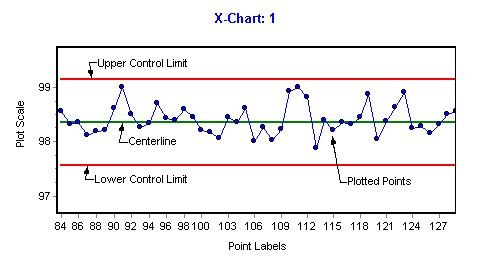
\includegraphics[height=0.3\textheight]{art/X-chartExample}
\caption[\barxChart]{\barxChart. \newline \url{https://mvpprograms.com/help/P-mvpstats/spc/WhatAreControlCharts}}
\label{fig:bar_x_chart}
\end{figure}



Figure~\ref{fig:bar_x_chart} makes it evident \barxChart requires us to make several design decisions.
A standard design decision is setting the centerline as the grand average of the process: 
\begin{align}
\label{eq:centerline}
	\hat{\mu}_0=1/\tau \sum_{t=1}^\tau \bar{x}_t,
\end{align}
where $\mu_0$ denotes the in-control mean of the process. 
Notation originates from treating the in-control process as a null hypothesis, as it should be thought of.


If it is unclear to you, how may we compute the grand average of a process that is still evolving and has not finished, you are right! We thus introduce the idea of \emph{Phase I} and \emph{Phase II}. \marginnote{Phase I/II}
Initially we assume the process it out of control, we identify and remove assignable causes of variation, until we are left with a ``well-behaved'' subset of data points, we believe to be in-control. We call this Phase I, and we use it to initialize required quantities such as the centre line. 
Eq.(\ref{eq:centerline}) thus implies that in Phase I we were left with $\tau$ samples assumingly in statistical control.
After the chart has been calibrated, and major assignable sources of variability removed, we can finally start monitoring the process, known as Phase II.



\begin{tcolorbox}[breakable]
\paragraph{Other design decisions}
\begin{enumerate}
\item Upper and lower confidence limits: UCL and LCL (do not confuse with USL and LSL!).
\item Sample size in each sample, denoted $n$.
\item The within period sampling scheme, known as \emph{rational groupings}.
\item The between-period sampling scheme, notably the \emph{frequency of samples}, denoted $h$. 
\item Other stopping rules.
\end{enumerate}
\end{tcolorbox}


These design decisions ultimately govern the error rates of the chart, which in turn, incur financial costs. 
For now we will restrict attention to type I/II error rates, until Section~\ref{sec:economical_considerations} where we consider these choices as economical optimization problems.

For ease of exposition, control chart design is demonstrated for the \barxChart, but equally applies to other control charts, presented in Section~\ref{sec:other_control_charts}.
We start by a type I error rate analysis. 
Denote $\alpha_t$ the false alarm probability at period $t$.
How do our design choices affect $\alpha_t$?
\begin{align}
	\alpha_t &:= 1-P_{H_0}(\bar{x}_t \in [LCL,UCL]) \\
	&= 2 P_{H_0}(\bar{x}_t<LCL) \\
	&= 2 P_{H_0}(Z<\frac{LCL-\mu}{\sigma_{\bar{x}}}) \\
	&= 2 P_{H_0}(Z < -\arm) \\
	&= 2 \Phi(-L)
\end{align}
The above follows from assuming that $UCL:=\mu_0 + \arm \sigmabar, LCL:= \mu_0 - \arm \sigmabar$, $\x_{it}\sim \gauss{\mu,\sigma^2}$, and denoting $\sigmabar:= \frac{\sigma}{\sqrt{n}}$.
A typical design choice is $\arm=3$, known as \emph{3-sigma control limits}, implying a false alarm rate of $\alpha_t=0.0027$.\marginnote{3-Sigma Control Limits}
Since we assumed the process is fixed over time, then so is $\alpha_t$ and we can simply write $\alpha_t=\alpha$.

\begin{remark}[3-Sigma Control Limits vs. 3-Sigma Capability]
Do not confuse these two similar ideas.
3-Sigma Control Limits is a statement on the false alarm rate of a process with respect to its own \textbf{history}.
3-Sigma Capability is a statement on the non-compliance rate of a process with respect to its \textbf{specification}.
\end{remark}


A power analysis for our design choices follows the same lines.
Denote by $H_1$ the out-of-control distribution,  $\beta_t$ the type-II error rate, and $\pi_t=1-\beta_t$ the power, at period $t$.
We then have
\begin{align}
	\pi_t &:= 1-P_{H_1}(\bar{x}_t \in [LCL,UCL])
\end{align}
and the rest follow from the distribution of $\bar{x}_t$ when the process is out of control.
Since the out-of-control shift is (asumingly) stable, we can again omit the time index and write $\pi=\pi_t$.
Assuming the out-of-control process is a shift of magnitude $k \sigma$, i.e.: $\x \sim_{H_1} \gauss{\mu_1,\sigma^2}; \mu_1=\mu_0+ k \sigma$, we plot in Figure~\ref{fig:power_function}, the detection power of a 3-sigma \barxChart, as a function of $k$. 
This is known in the statistical literature as a \emph{power function}, and in the engineering literature as the \emph{operator characteristic} (OC), or \emph{true positive rate operator characteristic}.\marginnote{Operator Characteristic}


\begin{figure}[h]
\centering
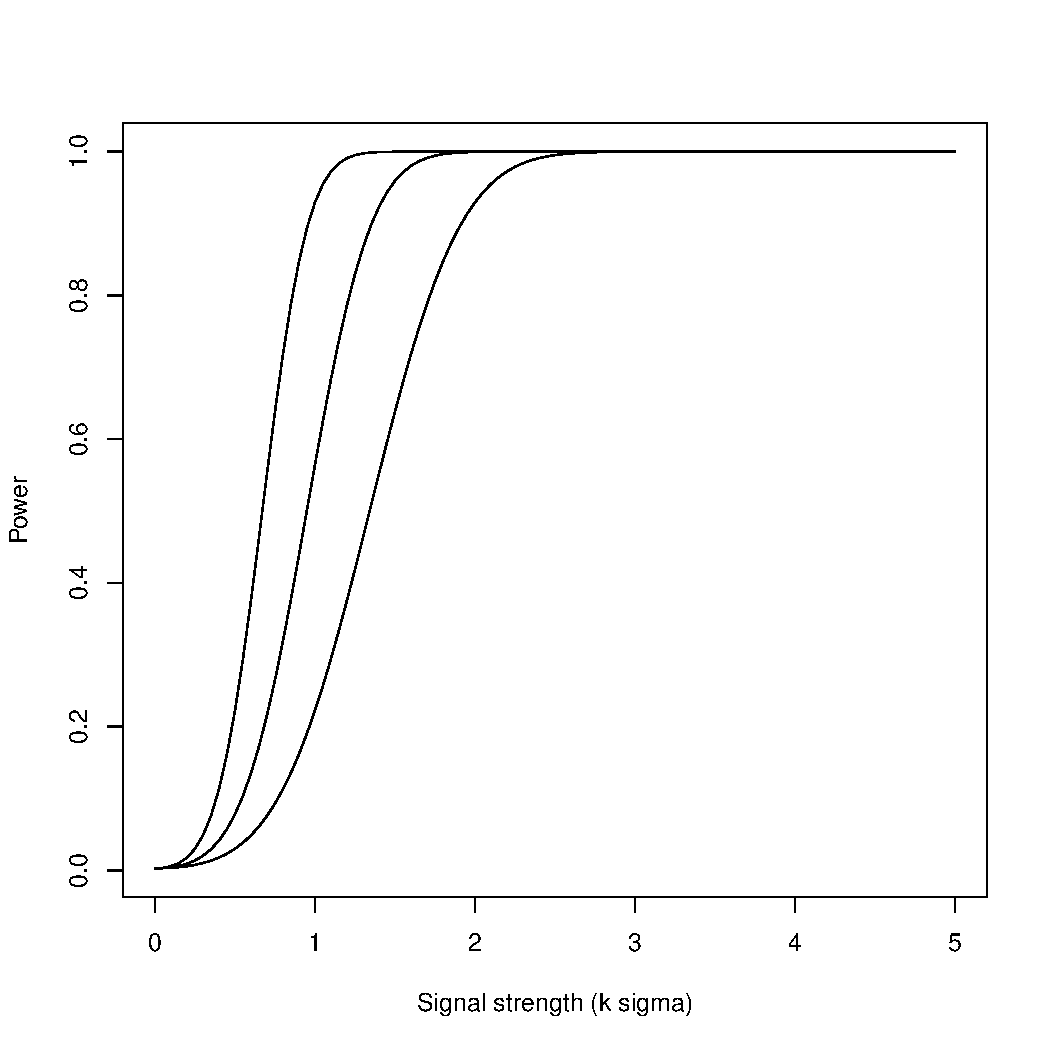
\includegraphics[height=0.3\textheight]{art/power_function.pdf}
\caption[Power Function]{Power function of the 3-sigma \barxChart with $n=5,10,20$ and $\mu_1=\mu_0 + k \sigma$.}
\label{fig:power_function}
\end{figure}

\begin{extra}[Operator Characteristics]
Many operator characteristics have been proposed to study the performance of control charts, statistical tests, or binary classifiers in general.
You may be already familiar with some, such as the ROC-curve. 
The curious reader is referred to \cite{wikipedia_receiver_2015} for more information.
\end{extra}


An important related quantity is the \emph{average run length} (ARL), which is the expected number of periods between two crossings of control limits, i.e., the expected periods between alarms. \marginnote{ARL}
We denote by $ARL_0$ the ARL when the process is under statistical control, and $ARL_1$ otherwise\footnote{Note that it is implied that the process has a \emph{stable} distribution, even though it is out if control.}. 
For Shewhart charts, where $\bar{x}_t$ are typically statistically independent, then clearly the number of periods until a crossing is geometrically distributed. Using the expectation of a geometric random variable we can conclude that 
\begin{align}
	ARL_0=1/\alpha \label{eq:arl_0}, \\
	ARL_1=1/\pi \label{eq:arl_1}.
\end{align}
Clearly we can convert to time units by multiplying the ARL by the duration of sampling interval.
This is known as the \emph{average time to signal} (ATS).\marginnote{ATS}
It is quite common to design a control chart so that it achieves a particular $ATS_0$.

\begin{remark}[ARLs more important than type-I errors]
In the case of Shewhart charts, there is a simple mapping between ARL and type I error rates.
This need not be the case for general control charts. 
Since type I errors are guaranteed if the process runs long enough, then it is actually the ARL that is more informative than type-I errors.
\end{remark}


Now assume that we are unhappy with our control chart. 
It simply makes too many false alarms, or takes too long to detect loss of statistical control.
What can we do about it?
Well, this is exactly the same question as when increasing the power or lowering the type I error of a statistical hypothesis test. This is obviously no coincidence, since control charts are nothing but a statistical test!
Here are some action courses:
\begin{enumerate}
\item Increase $\arm$. This is the same as shrinking the rejection region: 
it will decrease the false alarm rate, at the cost of power.
\item Increase $n$. Brilliant! Statistically, there is nothing to lose. It may, however, cost time and money.
\item Increase the sampling frequency. Brilliant again! Nothing to lose, except time and money...
\item Change the sampling scheme within period. We elaborate on this in Section~\ref{sec:rational_grouping}.
\item Add other stopping rules: 
this acts just like growing the rejection region. It will increase power, at the cost of type I error. We elaborate in Section~\ref{sec:stopping_rules}.
\item Pool together more time points or more CTQs. We elaborate on this in sections \ref{sec:running_windows} and  \ref{sec:multivariate}, respectively. 
\end{enumerate}






\subsection{Control Limits and the Alarm Rate}
As previously discussed, $\arm$ governs the tradeoff between type I and type II errors, or sensitivity versus specificity.
It is very common to set $\arm=3$. 
For a normally distributed CTQ, this implies $2,700$ false alarms per million periods. 
This also implies an $ARL_0$ of $1/\alpha \approx 370$ periods, which is conveniently, about a year when sampling once a day.
We may obviously, discard this $\arm=3$ convention, and directly set UCL and LCL so they guarantee some desirable false alarm rate, or ARL.

If normality of $\bar{x}_t$ can be assumed, then one may estimate $\sigma$ from phase I, and set LCL and UCL by finding the $\arm$ that solves $2\Phi(-\arm)=\alpha$.
If normality cannot be assumed, there are many ways to go about. Here are some options:
\begin{enumerate}
\item Increase $n$: even if $\x_{it}$ is non normal, for large enough $n$, then $\bar{x}_t$ will be via the central limit theorem (CLT).
\item Use empirical quantiles: If phase I was returned enough data, then we may estimate $\x_{\alpha/2}$ and $\x_{1-\alpha/2}$ using the empirical quantiles of phase I. The false alarm rate will be $\alpha$ since $P(\x \not \in [\hat{\x}_{\alpha/2},\hat{\x}_{1-\alpha/2}]) \approx \alpha$.
\item If some other distribution can be assumed then we may compute the false alarm rate of particular limits either analytically, or computationally (by simulation).
\end{enumerate}




\subsection{Rational Groupings}
\label{sec:rational_grouping}
Recall that at each period we compute the average of $n$ samples. 
How should we draw these samples? 
At the same time from the same machine?
At different times from the same machine?
Many configurations are possible, and the correct approach depends on the type of out-of-control behaviour one seeks. 
\emph{Rational groupings} merely reminds us to sample ``rationally'' in each period. 
Quoting \cite{montgomery_introduction_2007}'s words of caution:
\begin{quotation}
\dots we can often make any process appear to be in statistical control just by stretching out the interval between observations in the sample.
\end{quotation}






\subsection{Other Stopping Rules}
\label{sec:stopping_rules}

The assumption that we may only create alarms if $\bar{x}$ exceeds some control limits is needlessly restrictive.
A first relaxation is by allowing multiple control regions.
It is quite common to define \emph{warning limits} and \emph{action limits}. Each may have its own alarm rate.
We may even change the sapling scheme if limits are breached. Increasing the sampling rate once the warning limits have been breached is known as \emph{adaptive sampling}, or \emph{variable sampling}.\marginnote{Adaptive Sampling}



Another approach is to define multiple sets of stopping rules.
Here is an example:
\begin{enumerate}
\item One or more points outside of the 3-sigma control limits.
\item Two of three consecutive points outside the 2-sigma warning limits but still inside the 3-sigma control limits.
\item Four of five consecutive points beyond the 1-sigma limits.
\item A run of 8 consecutive points on one side of the centerline.
\end{enumerate}
The above set of rules is known as the Western Electric Rules, \aka, the \emph{WECO} rules.\marginnote{WECO}
Augmenting the set of rules is the same as increasing a rejection region. It adds more sensitivity, at the cost of false alarms. If the rules are properly selected, the gain in sensitivity is worth the increase in false alarms.

As a quick exercise, we may compute $\alpha$  for $m$ independent rules, each with $\alpha^*$ type I error:
\begin{align}
\label{eq:multiplicity_in_spc}
	\alpha=1-(1-\alpha^*)^m.
\end{align}
Having 4 rules, like WECO, each at $\alpha^*=0.0027$ implies that we actually have $\alpha=0.01$ and $ARL_0 \approx 93$. For daily sampling of an in-control process, this means an alarm every quarter, and not every year. 

\begin{extra}[Stopping Rules]
There are many sets of stopping rules. 
These include WECO, Nelson, AIAG, Juran, Hughes, Duncan, Gitlow, Westgard, and more. 
See \url{http://www.quinn-curtis.com/spcnamedrulesets.htm} for a quick review.
\end{extra}






\section{Pooling Information Over Periods}
\sectionmark{Pooling Periods}
\label{sec:running_windows}

Assume an out-of-control process is simply a mild shift of the controlled-process.
This shift may be hard to detect in Shewhart chart, especially if $n$ is not too large (as seen in Figure~\ref{fig:power_function}).  
If the shift persists over periods, we may gain power, i.e., sensitivity, by pooling several periods together. 
We now present several ways to pool information from history. These are typically applied in Phase II, where out-of-control processes are expected to have only mild shifts, and not major ones as in Phase I. 

\begin{remark}[No longer Shewhart]
The name \emph{Shewhart control chart} is reserved to charts plotting one period at a time. 
When several periods are pooled together, we will no longer call this  ``Shewhart''.
\end{remark}

\begin{remark}[One observation at a time]
The following charts have a continuous flavour. As such, it is both favourable, and common, to compute them using one observation at a time, meaning that $n=1$. 
\end{remark}



\subsection{Run Test Chart}
[TODO]




\subsection{Moving Average Chart (MA)}
\sectionmark{MA}

One way to pool information from different periods is by a \emph{moving average}.
\begin{definition}[MA]
The \emph{moving average} (MA) in a window $w$, at period $t$, is defined as
\begin{align}
	M_t:= \frac{x_t+\dots+x_{t-w+1}}{w}.
\end{align}
\end{definition}
Assuming $x_t \sim \gauss{\mu, \sigma_x^2}$ then clearly 
\begin{align}
	M_t \sim \gauss{\mu, \frac{\sigma_x^2}{w}}.
\end{align}

The control limits on $M_t$ are typically
\begin{align}
	UCL &:= \mu_0 + \arm \sigma_{M_t}= \mu_0 + \arm \, \frac{\sigma_x}{\sqrt{w}}, \\
	LCL &:= \mu_0 - \arm \sigma_{M_t}= \mu_0 - \arm \, \frac{\sigma_x}{\sqrt{w}}.
\end{align}
The false alarm rate of this criterion is trivially $\alpha=0.0027$. 
The $ARL_0$ is no longer simple to compute. 
This is because the pooling of periods has compromised independence between periods, and Eqs.(\ref{eq:arl_0},\ref{eq:arl_1}) are no longer valid. 
Do not despair as the ARL may still be computed. 
You can always use simulation to compute it, or try using the \rcode{spc} \R package.




We are free to choose the magnitude of $w$. 
If $w$ is too small, there is no real pooling from history. At the limit, where $w=1$, we are back to the classical Shewhart chart. 
If $w$ is too large, then each new observation has very small importance, and it may take a long time to detect a shift.
Which is the right intermediate value of $w$, is left for you to decide.






\subsection{Exponentially Weighted Moving Average Chart (EWMA)}
\sectionmark{EWMA}
The moving average gives all observations the same importance. 
We want to change this, giving more importance to new observations so that we may capture drifts quickly when they occur. 
The \emph{Exponentially Weighted Moving Average} (EWMA), \aka the \emph{geometric moving average} (GMA), does just that. \marginnote{GMA}
\begin{definition}[EWMA]
For a fixed $\lambda \in [0,1]$, the \emph{exponentially weighted moving average} (EWMA) is defined as 
\begin{align}
	z_t &:= \lambda x_t + (1-\lambda) z_{t-1}
\end{align}
\end{definition}
By recursive substitution, we have 
\begin{align}
	z_t &= \lambda \sum_{j=0}^{t-1} (1-\lambda)^j x_{t-j} + (1-\lambda)^t z_0,
\end{align}
and 
\begin{align}
\label{eq:ewma_variance}
	z_t &\sim \gauss{\mu_0,	\sigma^2_{z_t} }, \\
	\sigma^2_{z_t} &= \sigma^2_x \left( \frac{\lambda}{2-\lambda} \right)(1-(1-\lambda)^{2t}).
\end{align}
Eq.(\ref{eq:ewma_variance}) may be used to construct control limits for EWMA.
It is however, more economic to observe that for large $\lambda$ and $t$: $(1-(1-\lambda)^{2t}) \approx 1$ so that we may use 
\begin{align}
\begin{split}
\label{eq:ewma_variance_approximate}
	UCL &:= \mu_0 + \arm \sigma_{z_t} \approx \mu_0 + \arm \, \sqrt{\sigma^2_x\left( \frac{\lambda}{2-\lambda} \right)},  \\
	LCL &:= \mu_0 - \arm \sigma_{z_t} \approx \mu_0 - \arm \, \sqrt{\sigma^2_x\left( \frac{\lambda}{2-\lambda} \right)},
\end{split}
\end{align}
with $\arm=3$ being the typical choice.
By now, you should immediately know what is the false alarm rate of these limits.
By now, you should also know that because of the dependence between $z_t$'s, computing the ARL is not as simple as for Shewhart charts. The \rcode{xewma.arl()} \R function, in package \rcode{spc}, permits doing so easily. 
Its output for various $\lambda$ and $\arm$ is illustrated in Figure~\ref{fig:arl_0_ewma}.

\begin{figure}[h]
\centering
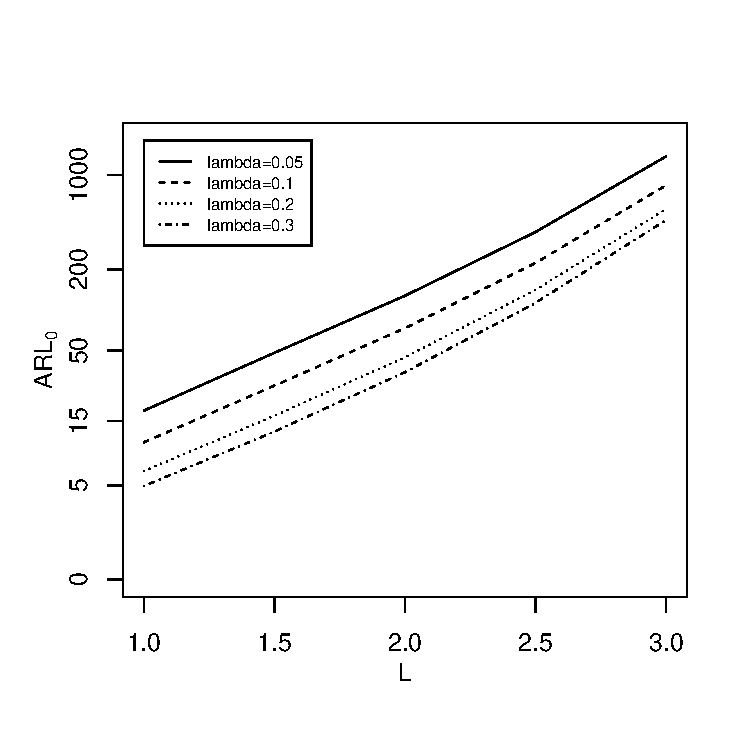
\includegraphics[height=0.3\textheight]{art/fig53}
\caption[$ARL_0$ for EWMA]{$ARL_0$ for EWMA. \newline Code from \url{http://users.phhp.ufl.edu/pqiu/research/book/spc/r-codes/fig53.r}}
\label{fig:arl_0_ewma}
\end{figure}

In the MA chart, we used the choice of $w$ to balance between quick response (small $w$) and sensitivity (large $w$).
EWMA has no window-width parameter, since it looks into all of history. On the other hand, we can control it by choosing $\lambda$. 
Large $\lambda$ gives more importance to the present. At the limit, $\lambda=1$, EWMA collapses to a standard Shewhart chart.







\subsection{Filtered Derivative Chart}
[TODO]


\subsection[CUSUM]{CUSUM Chart}
The \emph{cumulative sum} chart is similar to the EWMA in that it pools information from the history. 
The CUSUM simply sums all past deviations from the centre line.
If the process is in control, deviation will cancel each other, and their sum will vary around $0$. 
If the process is out of control, a drift will appear. 
The statistic to be plotted is 
\begin{align}
	C_t:= \sum_{j=0}^{t}(x_j-\mu_0)=C_{t-1}+ (x_t-\mu_0)
\end{align} 
Observing that when under control then $C_t \sim \gauss{\mu_0, t \sigma_x^2}$, we could set 
\begin{align}
\label{eq:cusum_simple_limits}
\begin{split}
	UCL &:= \mu_0 + \arm \sigma_{C_t}= \mu_0 + \arm \, \sqrt{t \sigma_x^2},  \\
	LCL &:= \mu_0 - \arm \sigma_{C_t}= \mu_0 - \arm \, \sqrt{t \sigma_x^2}.
\end{split}
\end{align}
\DIFaddbegin 

\begin{extra}
\DIFaddend You may encounter these limits in your favourite software (\rcode{qcc} package in \R), but it less often discussed in the literature. 
This is because CUSUMs were introduced by \cite{page_continuous_1954}, which offered different control limits. 
\cite{montgomery_introduction_2007} adopts \citeauthor{page_continuous_1954}'s view and presents limits in two forms: the \emph{decision interval} (DI) form, \aka the \emph{tabular} form, and the graphical form known as a \emph{V-mask}.\marginnote{V-Mask}
These two control limits are equivalent. Before we present them, we try to offer some intuition for the difference between the limits in Eq.(\ref{eq:cusum_simple_limits}) and those of \cite{page_continuous_1954}.
\DIFdelbegin %DIFDELCMD < 

%DIFDELCMD < %%%
\DIFdelend The fundamental difference between the control limits of \cite{page_continuous_1954}, and the ones presented until now, is that \citeauthor{page_continuous_1954} designed limits for the particular history of each process, while the limits until now, including Eq.(\ref{eq:cusum_simple_limits}) do not adapt to the particular history of the process.
As such, \citeauthor{page_continuous_1954}'s control limits are said to be \emph{adaptive}.\marginnote{Adaptive Contol Limits}
\DIFaddbegin \end{extra}
\DIFaddend 






\DIFdelbegin %DIFDELCMD < [%%%
\DIFdel{TODO: explain V-mask and tabular}%DIFDELCMD < ]
%DIFDELCMD < 

%DIFDELCMD < %%%
\DIFdelend \subsection{Shiryaev-Roberts Procedure}
[TODO]





\subsection{Combined Shewhart and Running Window Charts}
Well sure- if you want to enjoy the quick detection of Shewhart charts, and the sensitivity of running windows charts, you may certainly design charts that marry these ideas.
False alarm rates and ARLs should be computed mutatis mutandis.







\section[Multivariate]{Multivariate Control Charts}
\label{sec:multivariate}

\begin{example}[Intensive Care Unit]
\label{eg:intensive}
Consider an intensive care unit. 
The CTQs are the patient's blood pressure, temperature, etc.
We want to sound an alarm if the patient's condition deteriorates. 
Clearly, we can apply the univariate methodology above on each CTQ.
It is possible, that the deterioration is mild, so that it is not picked up by any CTQ individually (low power), but could have been noticed were we to aggregate signal over various CTQs. 
This is the concern of the current section. 
\end{example}


\subsection{Mass Univariate Control}
\label{sec:mass_univariate}

A first natural approach is to raise an alarm when \textbf{any} of the processes exceeds its respective control limits.
For \DIFdelbegin \DIFdel{$m$ }\DIFdelend \DIFaddbegin \DIFadd{$p$ }\DIFaddend independent processes, with false alarm rate $\alpha^*$ each, then the joint false alarm rate is 
\begin{align}
	\alpha  = 1-(1-\alpha^*){^p}.
\end{align}
Clearly we could set \DIFdelbegin \DIFdel{$\alpha^*=1-\sqrt[m]{1-\alpha}$}\DIFdelend \DIFaddbegin \DIFadd{$\alpha^*=1-\sqrt[p]{1-\alpha}$}\DIFaddend , so that the joint false alarm rate is under control, but we would not be enjoying the added sensitivity of pooling many CTQs together. 



\subsection{Hotteling's \tsq}
Hotteling's \tsq statistic is a generalization of the t-test.
To see this we write the t-statistic in the following weird form:
\begin{align}
	t^2_t(x)=(\bar{x}_t-\mu_0) (s^2_t(x))^{-1} (\bar{x}_t-\mu_0).
\end{align}
This notation readily extends to the multivariate case. 
For $p$ CTQs, then $\bar{x}_t$ and $\mu_0$ are $p$-length vectors, and $s^2_t(x)$ is replaced with the $p \times p$ covariance matrix $\hat{\Sigma}_t(x)$.
\begin{definition}[Hotteling's \tsq]
\begin{align}
\label{eq:hotteling}
	T^2_t := n (\bar{x}_t-\hat{\mu}_0)' \hat{\Sigma}^{-1} (\bar{x}_t-\hat{\mu}_0).
\end{align}
\end{definition}
To derive the control limits, we will be assuming that $\x_{it}$ is $p$-variate Gaussian distributed, $\x_{it}\sim \gauss{\mu_0, \Sigma_{p \times p}}$. 
The sampling distribution of $T^2_t$ will depend on how $\mu_0$ and $\Sigma_t$ are estimated. 
In a wide variety of cases, when the number of observations for estimation is much larger then $p^2$, then 
\begin{align}
	T^2_t \overset{H_0}{\rightsquigarrow }\chi^2_p.
\end{align}
We can thus construct the control limit for this scenario:
\begin{align}
	UCL:= \chi^2_{1-\alpha,p}.
\end{align}
Note that the \tsq statistic is \emph{non directional}: it will increase in the presence of both positive and negative drift, so that there is no LCL.

We may consider the exact distribution of \tsq under many configurations. 
We opted for the $\chi^2_p$ for ease of exposition. For exact result \cite[Ch.7]{qiu_introduction_2013} should be consulted. 

Since the above limits have an (approximate) type-I error rate of $\alpha$, and the periods are typically independent, then we can readily apply Eq.(\ref{eq:arl_0}) to compute $ARL_0$.



\subsection{Other Pooling Statistics}
Hotteling's \tsq implicitly targets a weak signal on many coordinates. 
In the signal detection literature, this is known as a \emph{dense} signal.
In our intensive care unit example (Example~\ref{eg:intensive}), it may be the case that a patient's deterioration is mildly manifested in many CTQs. It may however, be the case, that deterioration is manifested in a small subset of CTQs.
This is further emphasized in Example~\ref{eg:cyber}.

\begin{example}[Cyber Monitoring System]
\label{eg:cyber}
Consider a server farm. All servers dump their status into logs. These include CPU loads, temperature, network I/O, etc.
The administrator is worried about an imminent attack, and is thus parsing the logs for CTQs, and inspecting the on-line status on his dashboard.
He knows that the cyber-attacker is no amateur, so that if any fingerprint is left in the logs, it will be very subtle and manifested in very few CTQs\footnote{Clearly, these are not called CTQs, in this context. We are simply adhering to notation.}.
\end{example}

The intensive care example, and the cyber security example, motivate our search for a statistic, that unlike Hotteling's \tsq, is sensitive to \emph{sparse} signals. \marginnote{Sparse Signal}
I.e., a signal that is manifested in very few of the $p$ CTQs.
For this purpose, we merely offer several candidate multivariate statistics, with references where appropriate.
\begin{description}
\item [Max pooling] Where we control the process using the $\max$ over CTQs. Useful when we expect signal in a handful of CTQs. This is in fact identical to the mass univariate approach of Section~\ref{sec:mass_univariate}.
\item [Higher Criticism] Where pooling is performed using the Higher Criticism statistic. Appropriate for an intermediate \emph{rare-weak} sparsity pattern. See details in \citep{jin_cosmological_2005}.
\item [Skewness Statistic] Where pooling is performed using the empirical third moment. Appropriate for an intermediate sparsity pattern. See details in \citep{jin_cosmological_2005}.
\end{description}







\section{Economical Design of Control Charts}
\label{sec:economical_considerations}

Up until now, our design of control charts was driven by type-I error rates, and ARLs. Economical consideration were merely implied.
In this section, economical consideration take the driver's seat. 
We present a toy model, to demonstrate the economical optimization of design parameters in a \barxChart. 
Before beginning, a few remarks are in order. 

\begin{remark}[Economical Design of Control Charts]
\noindent
\begin{enumerate}
\item According to \cite{montgomery_introduction_2007} 
\begin{quote}
Saniga and Shirland (1977) and Chiu and Wetherill (1975) report that \textbf{very few practitioners} have implemented economic models for the design of control charts.
\end{quote}
Hmmmm.. Have things changed since 1977?
\item A comprehensive theoretical analysis of the optimization of a quality control system may be found in \cite{girshick_bayes_1952}. Again, \cite{montgomery_introduction_2007} is skeptic:
\begin{quote}
The optimal control rules are difficult to derive, as they depend on the solution to complex integral equations. Consequently, \textbf{the model’s use in practice has been very limited}.
\end{quote}
\end{enumerate}
\end{remark}

In light of the above skepticism, and following the lines of \cite{duncan_economic_1956}, we aim at the modest goal of an economical optimal \barxChart. 
Our target function is optimizing the expected income per hour, with respect to the design parameters:
\begin{align}
\label{eq:optimal_design}
	\max_{n,\arm,h}\set{\expect{C/T}}
\end{align}
where $C$ is the income between two productions halts, i.e., a \emph{cycle};
$T$ is the cycle duration;
$n$ is the number of samples per period;
$\arm$ governs the control limits via $UCL:= \mu_0+ \arm \sigma_{\bar{x}}= \mu_0+ \arm \sigma_x / \sqrt{n}$;
$h$ is the hours between sample periods. 

We now need to establish how $\expect{C/T}$ is related to $n,\arm,h$. Here is our set of assumptions and notation:
\begin{enumerate}
\item When in control (IC), production is centred on $\mu_0$, assumed known. 
\item When out of control (OC), $\mu_1=\mu_0 \pm k \sigma_x$. 
\item When OC, production may proceed (!). 
\item Search and repair costs are not part of $C$.
\item OCs occur as a Poisson process, with rate $\lambda$ events per hour. The expected time from a sampling to an OC events is thus 
\begin{align}
	\tau := \frac{1-(1+ \lambda h) e^{-\lambda h}}{\lambda(1-e^{-\lambda h})}.
\end{align} 
\item The power to detect an OC is 
\begin{align}
	\pi:= \Phi(-\arm-k/\sqrt{n})+ (1-\Phi(\arm-k/\sqrt{n})).
\end{align}
\item The false alarm rate
\begin{align}
	\alpha:= 2 \Phi(-\arm).
\end{align}
\item Because of the Poisson process assumption,  $\expect{C/T}=\expect{C}/\expect{T}$. 
\item The expected cycle length:
\begin{align}
	\expect{T}= \frac{1}{\lambda}+ \frac{h}{\pi}- \tau  + D.
\end{align}
where $\frac{1}{\lambda}$ is time IC;
$\frac{h}{\pi}- \tau$ is the time the process is OC until detection;
$D$ is a fixed time to identify the assignable cause. 
\item The expected income per cycle
\begin{align*}
	\expect{C}= V_0 \frac{1}{\lambda} + 
	V_1 \left(\frac{h}{\pi}- \tau  + D  \right) - 
	a_3 -
	\frac{a'_3 e^{-\lambda h}}{1-e^{-\lambda h}} -
	(a_1+a_2n)\frac{\expect{T}}{h}
\end{align*}
where $V_0$ is the net income per cycle when IC;
$V_1$ is the net income when OC;
$(a_1+a_2n)$ is the fixed and variable cost of taking a sample;
$a_3$ is the cost of finding an assignable cause;
$a'_3$ is the cost of investigating a false alarm.
\end{enumerate}

[TODO: add timeline]

Given all the above, we may now plug Eq.(\ref{eq:optimal_design}) into our favourite numerical solver to find the optimal $h,\arm,n$.



\section{Shewhart Charts With Other Test Statistics}

We have been focusing on the \barxChart for ease of exposition. There are, however, many cases where the mean is not an appropriate test statistic.
Examples include:
\begin{enumerate}
\item A discrete CTQ, where only the number of non-compliances can be counted. 
\item Where the departure from statistical control is not only a shift in $\mu$.
\end{enumerate}

The following charts are designed for those cases. 
Practically all of the ideas presented for the \barxChart may be adapted to these other test statistics after appropriate adaptations. 
The reader is referred to \cite{montgomery_introduction_2007} for the details. 

\label{sec:other_control_charts}
\subsection{$R$ Chart}
Where $\bar{x}$ is replaced by the range, $\max_i\set{x_{i,t}}-\min_i\set{x_{i,t}}$.
Sensitive to variability changes. 
Popularized by its ease of implementation, in the pre-computer age. 
\subsection{$s$ Chart}
Where $\bar{x}$ is replaced by $s$. 
Sensitive to variability changes. 
Usually more sensitive than the range.
\subsection{$s^2$ Chart}
Like the $s$ chart, only in variance-scale.
\subsection{$p$ and $np$ Chart}
Where $\bar{x}$ is replaced by the proportion ($p$), or number ($np$), of non-conforming units.
Appropriate for attributes, i.e., discrete CTQs.
\subsection{$c$ Chart}
Like a $np$ chart, but where the number of nonconforming units is replaced with the total number of nonconformances, allowing multiple defects per unit. 
\subsection{$u$ Chart}
Like the $c$ chart, but allowing a variable number of units per period (varying $n$).
\subsection{Regression Control Chart}
In a \emph{regression control chart}, the test statistic can be a regression coefficient. 
When compounded with multivariate charts, a regression control chart may accommodate several regression  coefficient, or the residuals. 




\section[Extensions]{Extensions of Control Charts}
We have been discussing the simplest of \barxChart, for ease of exposition.
Several immediate extensions are possible.
The reader is referred to \cite{montgomery_introduction_2007} for details.
\begin{description}

\item [One sided charts] Just like hypothesis testing, where we may consider non-directional or directional hypotheses, we may consider directional control chart. 
Obviously the control limits and the test statistic may need appropriate updates.

\item [Autocorrelation and time series models] The assumption of independence between sampling periods may be relaxed, by adopting a quantitative or qualitative model for temporal dependence.

\item [Running windows] The ideas of pooling information over periods with a MA, EWMA, and CUSUM may be extended to all type of Shewhart charts. 
Also, there are endlessly many period pooling schemes. 
You are free to pick a set of weights, or convolve your data with a \emph{causal filter}\footnote{\url{https://en.wikipedia.org/wiki/Causal_filter}} to create your favourite pooling scheme.

\item [Multiple Charts] When inspecting a process, rarely does one inspect a single chart at a time. A typical dashboard would include several charts running in parallel, as depicted in Figure~\ref{fig:dashboard}.

\end{description}



\subsection{Cuescore Charts}
[TODO]



\section{Bibliographic Notes}
The contents of this chapter is mostly derived from \cite{montgomery_introduction_2007}. 
For a more mathematically rigorous treatment of the topic see \cite{basseville_detection_1993}.
For an \R oriented exposition of the topic, see \cite{qiu_introduction_2013}.
A quick digest review may be found in \cite{natrella_nist/sematech_2010}.
For multivariate process control, see for example \cite{ge_multivariate_2012}. 



\chapter{Design of Experiments}
\chaptermark{DOE}

This chapter is devoted to the matter of designing experiments, and follows the lines of \cite{cox_theory_2000}.
A control chart may be seen as an on-line experiment alerting us when the milk goes sour, but it will not tell us why. 
When designing a product (remember DFSS \ref{sec:dfss}), or once a control chart has signalled an alert, we will want to know what has influences our production, and how to remove variability.
In our SPC terminology, we will want to know what are the \emph{causal} \emph{effects} of our \emph{controllable inputs} (or \emph{factors}), on our \emph{CTQ} (or \emph{response}). 
The theory of discovering these effects is the theory of \emph{design of experiments} (DOE).
Its goal is to \emph{screen} factors with no effect, to estimate effect sizes, and find optimal factor-level combinations, and remove assignable variability; all these as efficiently as possibly.



Roughly speaking, the challenges in designing good experiment are:
\begin{enumerate}
\item Efficiency: extract the most information per sampled unit.
\item Signal to noise: remove variability that might mask factor effects.
\item Bias: avoid uncontrolled effects from being ``absorbed'' into controlled ones.
\end{enumerate}





Before we dig in, several matters should be emphasized:
\begin{description}
\item [Randomization] Randomization is fundamental to our purpose. This is because the idea of an \emph{effect} implies causality. Any inference we make, is causal, which is the inference we need for controlling a process.
It is the mechanism of randomization, that allows us to conclude that correlations are causal, and not merely statistical.
For a treatment of causal inference in \emph{observational data}, i.e., without randomization, see \cite{rosenbaum_observational_2002}.

\item [Pre-experiment] In this text we take it for granted that the purpose of the experiment is well known, and the candidate factors defined. We are fully aware, as should be the reader, that in application this is a non-trivial luxury. Indeed, a lot of planning, and domain-knowledge go into the selection of factors, their candidate levels, etc.

\item [Power Analysis] Part of the pre-experiment may include a power analysis. The pre-experiment power analysis will typically be very approximate, and rely on many assumptions. It is still important, as it gives an idea of the feasibility of an experiment, and avoids wasting resources.

\item [No Textbook Solution] We will present many design ideas and principles, yet it should be emphasized that real life problems rarely obey text-books. You should thus feel free, and even obliged, to think about your particular problem and adapt the experiment as you best see fit. 

\item[Data Analysis]
In this text, we only discuss the \textbf{design} of the experiment, and not the \textbf{analysis} of the data.
This is a non-standard choice as DOE is typically presented alongside the \emph{analysis of variance} (ANOVA) framework.\marginnote{ANOVA}
We decouple the two since: 
\cite{cox_theory_2000} do so, 
these are two different thing, and finally because the ANOVA framework may be easily replaced by the framework of \emph{linear models}, \emph{mixed models}, \emph{variance components}, and possibly others. 
There is a vast literature focusing on the analysis method. \marginnote{Linear Models, \\ Mixed Models, Variance Components}
If asked, this author may recommend \cite{hocking_analysis_1985}, which presents both the ANOVA terminology, and the linear models terminology.
That book, however, may be hard to come by, so feel free to ask me for other references if required.

\end{description}








\section{Terminology}
The following list is compiled from \cite{mason_statistical_2003}. Many, if not most of the following terms, originate in R.A. Fisher's seminal book ``The Design of Experiments'' \citep{fisher_design_1960}. As usual, when old ideas get new names, we try to emphasize this in the text.



\begin{description}

\item [Experimental Unit]  Entity on which a measurement or an observation is made;
sometimes refers to the actual measurement or observation.
\item [Homogenous Experimental Unit] Units that are as uniform as possible on all characteristics that could affect the response.

\item [Factors]  A controllable experimental variable that is thought to influence the response. In the language of SPC: \emph{a controllable input}.

\item [Level] Specific value of a factor.

\item[Treatment] The particular factor-level combination applied to an experimental unit. \Aka \emph{manipulation}, or \emph{cell}.

\item [Factor Encodings] The numerical encoding of factor levels.
Of minor importance for designing. Of major importance for analysis.
Two level factor encodings include:
\begin{enumerate}
\item Effect coding: where levels are encoded with $\set{-1,1}$.
\item Dummy coding: where levels are encoded with $\set{0,1}$.
\end{enumerate}

\item [Experimental Region] All possible factor–level combinations for which experimentation is possible. \Aka \emph{factor space}, and \emph{design region}.

\item [Design Matrix] A matrix description of an experiment that is useful for constructing and analyzing experiments.

\item [Response] The CTQ in the SPC literature. 

\item [Main Effect] Change in the expected response between two factor–levels.  
We emphasize that effects, unlike simple population parameters, imply a causal relationship.
Part of the \emph{assignable causes} in the SPC literature.

\item [Interaction] Existence of joint factor effects in which the effect of each factor depends on the levels of the other factors.
Part of the \emph{assignable causes} in the SPC literature.

\item [Noise] \Aka \emph{error}. The part of the response that cannot be attributed to any factors.
This is the \emph{common} variability in the SPC literature.

\item [Replication] Repetition of an entire experiment or a portion of an experiment under two or more sets of conditions.

\item [Covariate]  An uncontrollable variable that influences the response but is unaffected by any other experimental factors.
\Aka an \emph{exogenous} variable in the econometric literature.

\item [Non Specific Factor] A variable that we suspect to affect the response, but we can only vaguely define, thus impossible to measure. As a consequence, we will not care to study its effect, but rather just remove it (e.g. by blocking). 


\item [Design]  Complete specification of experimental test runs, including blocking, randomization, repeat tests, replication, and the assignment of factor–level combinations to experimental units.

\item [Blocking]  Blocking, or \emph{grouping}, is an experimental design technique that removes excess variation by grouping experimental units or test runs so that those units or test runs within a block are more homogeneous than those in different blocks. Blocking attributes are also known as \emph{non specific factors}.\marginnote{Non Specific Factors}

\item [Confounding] When the design is such that several effects cannot be told apart. \Aka \emph{aliasing}.

\item [Repeat Tests] Two or more observations that have the same levels for all the factors, i.e., receive the same treatment.

\item [Balance] Some symmetry in the combinatorial design of the experiment. In its simplest interpretation, a design where an equal number of units is assigned to each treatment.

\item [Orthogonality]  Special simplifications of analysis and achievement of efficiency consequent on such \emph{balance}.
\end{description}








\section{Dealing with Variability}
\label{sec:variance_components}

The idea that random samples come with variability, or noise, should not be new to the reader.
In this section, we will try to decompose variability into it sources, and learn several techniques to reduce them. 
Starting with a motivating example.



\begin{example}[Web Design]
\label{eg:variance_components}
Consider the problem of optimizing a web site, or user interface, where individuals performance is measured by conversion rate (the probability of a new user to signup, purchase, etc).
Users' conversion is influenced by several factors:
The site's attributes,
the users' attributes, 
a user's affinity to a particular attributes,  
a user's mood, 
and endlessly many other things
How can we accurately optimize our site, in the presence of these variability sources?
The site's attributes are the \emph{factors} we want to study.
The users' attributes are \emph{covariates}. 
A user's affinity to the site's attributes is an \emph{interaction}. 
The users' mood is unobservable, thus a \emph{non-specific factor} we will try to either \emph{block} or \emph{balance}.
Any other variability, will be captured by the \emph{noise} term of the model. 
\end{example}


In this chapter we will learn many principled methods for the efficient design of experiments which allow us to remove effect-masking variability, avoid bias, and reduce costs.
You may, and should, think of this web design problem as we advance, since all the methods presented may be applied to it.



\subsection{Gage R\&R Studies}
R\&R stands for \emph{repeatability} and \emph{reproducibility}.
In the context of quality control\footnote{Beware that these words are used with different meanings by different communities.} repeatability is the variability under repeated measurement, and reproducibility is the variability when the same measurement is performed elsewhere (different lab, technician, etc.).
Gage R\&R experiments consist of performing several \emph{repeat tests}, and different replications, in order to assess R\&R, which can be thought of the assessment of the precision of the experiment. 



\subsection{Completely Randomized Designs}
In the simplest of designs, all experimental units are randomly assigned to treatments. 
This is typically easy to implement.
In Example~\ref{eg:variance_components} this would imply randomly assigning users to interfaces.
If you suspect, as you should, that we may reduce variability by grouping types of users together, keep reading.



\subsection{Randomized Block Designs}
The idea of \emph{blocking} is to replace the complete randomization scheme by a restricted randomization scheme so that variability can be reduced without introducing bias. 
The restricted randomization is created by \emph{grouping}, or \emph{blocking} groups of experimental units, and randomizing allocation within the group. 
In our running example, we could reduce the variability of the web site's attributes by showing various sites to the same person- each person would be his own block. This is an example of \emph{crossover} design, discussed in Section~\ref{sec:crossover}.
Alternatively, we could block individuals along, say, age group. Age would act as a a non-specific factor, and we would then randomly assign user's to sites, only within age groups.
If each age group has as many users as there are different site designs, this is a \emph{randomized complete block design}.\marginnote{Complete Block Design}
If there are less users then site designs, this is a \emph{incomplete block design}.
There are several approaches to incomplete block designs, but we refer the reader to \cite[Sec.4.2]{cox_theory_2000} for details.




\subsubsection{Latin Square Design}
When homogenous groups are defined by two non-specific factors, we would like to create blocks that are balanced, so that the non-specific factors do not bias effect estiamtes.
In our running example, non-specific factors may be age and gender. 
We could construct all age and gender combinations, and randomly assign users from each age-gender to each site design.
This would is an example of a \emph{split plot} design, discussed in Section~\ref{sec:split_plot}.
If, however, we do not deal with age-gender, but rather with age-country, we may not have enough users in each cell to assign to all site designs. 
Since we do not want to estimate the effect of age, nor country, but merely balance the design so that age and country effects do not alias the site's effect, we do not actually need all age-country combinations. 



If we have $k$ designs, we may group ages and countries into $k$ categories each, and each design is seen only once in each age group and once in each country group. 
This allocation of treatment to blocks is known as a \emph{Latin Square}. 
Table~\ref{tab:latin_square} demonstrates a Latin Square for $7$ web site designs, and compares it to a non-balanced allocation. 
\begin{table}[ht]
    \begin{minipage}{.5\linewidth}
        \centering
		\begin{tabular}{rlllllll}
		  \hline
		 & 1 & 2 & 3 & 4 & 5 & 6 & 7 \\ 
		  \hline
		1 & 1 & 2 & 3 & 4 & 5 & 6 & 7 \\ 
		2 & 1 & 2 & 3 & 4 & 5 & 6 & 7 \\ 
		3 & 1 & 2 & 3 & 4 & 5 & 6 & 7 \\ 
		4 & 1 & 2 & 3 & 4 & 5 & 6 & 7 \\ 
		5 & 1 & 2 & 3 & 4 & 5 & 6 & 7 \\ 
		6 & 1 & 2 & 3 & 4 & 5 & 6 & 7 \\ 
		7 & 1 & 2 & 3 & 4 & 5 & 6 & 7 \\ 
		   \hline
		\end{tabular}
    \end{minipage}    \begin{minipage}{.5\linewidth}
      \centering
		\begin{tabular}{rlllllll}
		  \hline
		 & 1 & 2 & 3 & 4 & 5 & 6 & 7 \\ 
		  \hline
		1 & 1 & 2 & 3 & 4 & 5 & 6 & 7 \\ 
		  2 & 2 & 3 & 4 & 5 & 6 & 7 & 1 \\ 
		  3 & 3 & 4 & 5 & 6 & 7 & 1 & 2 \\ 
		  4 & 4 & 5 & 6 & 7 & 1 & 2 & 3 \\ 
		  5 & 5 & 6 & 7 & 1 & 2 & 3 & 4 \\ 
		  6 & 6 & 7 & 1 & 2 & 3 & 4 & 5 \\ 
		  7 & 7 & 1 & 2 & 3 & 4 & 5 & 6 \\ 
		   \hline
		\end{tabular}
		\end{minipage} 
	\caption{A $7$-treatment, two-factor design. 
	Left pane is not balanced.
	Right pane is balanced with a Latin Square, generated with the \rcode{MOLS()} function of the \rcode{crossdes} \R package.}
	\label{tab:latin_square}		
\end{table}


The following example makes the same point, with the original agricultural motivation for this design.
\begin{example}[Agricultural Yield Study]
\label{eg:latin_square}
Consider an farmer growing corn.
He wishes to study the effect of $7$ candidate fertilizers (single factor with $7$ levels).
He is aware that the location of the plot may affect yield, due to slightly different sunlight, irrigation, altitude, etc.
He thus assumes he has to deal with two extra variance sources: row and column of the plot. 
He could treat the row and column as two factors, with $7$ levels each, be he does not care to estimate the row/column effect, but merely to avoid bias.
He will thus try to look for an allocation of fertilizer to rows and columns so that any row/column effect will be averaged out.
The Latin Square design of Table~\ref{tab:latin_square} does just that.
\end{example}


\begin{extra}\noindent
\begin{enumerate}
\item If the Latin Square reminds you of Soduko, it should. Soduko is just that!
\item The Latin Square is a very economical design, and is not used as often as it should be.
\item If we had reason to believe that different age groups in different countries respond differently to each site (an interaction), then the Latin Square may actually introduce aliasing. 
\end{enumerate}
\end{extra}



\subsubsection{Extensions of the Latin Square}
\begin{enumerate}
\item \textbf{Latin Hypercube}: When balancing more than two non-specific factors, we will call upon \emph{latin hypercube designs}, \aka \emph{orthogonal latin squares}. \marginnote{Orthogonal Latin Squares}
\item \textbf{Greco-Latin Square}: A latin-hypercube with three variability sources. 
\end{enumerate}






\subsubsection{Crossover Design}
\label{sec:crossover}
Lets return to the web site layout example (\ref{eg:variance_components}).
Let us also assume that our site has $3$ web pages. A landing page, an information page, and a form to fill. 
It is possible that the response to a particular page is affected by the previous page presented. 
This is known as a \emph{carryover effecf}, or \emph{residual effect}, which may bias the main layout effects of interest. \marginnote{Carryover Effect}

The more general phenomenon is dependence in the noise between trials. 
Consider the same subject undergoing different treatments, or adjacent fields. 
\emph{Crossover} designs are such that all possible treatment adjacencies are considered, so that the carry over effect averages out. 

In a \emph{fully randomized crossover design}, each unit is randomly allocated to a sequence of treatments.
If treatments are combinations of several factors, it is not uncommon to use Latin Squares to generate the sequences. Table~\ref{tab:crossover} demonstrates the $3!=6$ sequences for our $3$ page website problem.
\begin{table}[ht]
\centering
\begin{tabular}{rlll}
  \hline
 & 1 & 2 & 3 \\ 
  \hline
1 & 1 & 2 & 3 \\ 
  2 & 2 & 3 & 1 \\ 
  3 & 3 & 1 & 2 \\ 
  4 & 1 & 3 & 2 \\ 
  5 & 2 & 1 & 3 \\ 
  6 & 3 & 2 & 1 \\ 
   \hline
\end{tabular}
\caption[Crossover Design]{Crossover design: a balanced sequence of administration of $3$ treatments, generated with the \rcode{des.MOLS()} function of the \rcode{crossdes} \R package. }
\label{tab:crossover}
\end{table}






\section{Factorial Designs}
Until now we discussed some arbitrary set of treatments.
It is quite common, is not certain, that the many treatments are merely combination of a small number of \emph{factors} with a small number of \emph{levels} each.
This means that we may decompose treatment effect into the (partial) sums of the effects of underlying factors, which would make both the design more economical, and the analysis easier to interpret.

We will now present several designs for factorial experiments.
Recall that factors define treatments. The noise reducing and bias avoiding methods of Section~\ref{sec:variance_components} may thus be compounded with the treatment generating methods of this section.

It should be emphasized that a factorial design is better than $k$ experiments with one factor at a time. This is because:
\begin{enumerate}
\item Factorial experiments are make better (statistical) use of each sample unit for estimating main effects.
\item Factorial experiments allow the estimation of interactions between factors. 
\end{enumerate}
A classical illustration of the second point, is given in Figure~\ref{fig:one_factor_at_a_time}.
The figure depicts a one-factor-at-a-time optimization sequence (from A to H). Since the factors are not varied simultaneously, the experiments is unable to identify that the response is not a linear surface. 
Put differently, he is unable to estimate an interaction.

\begin{figure}[ht]
\centering
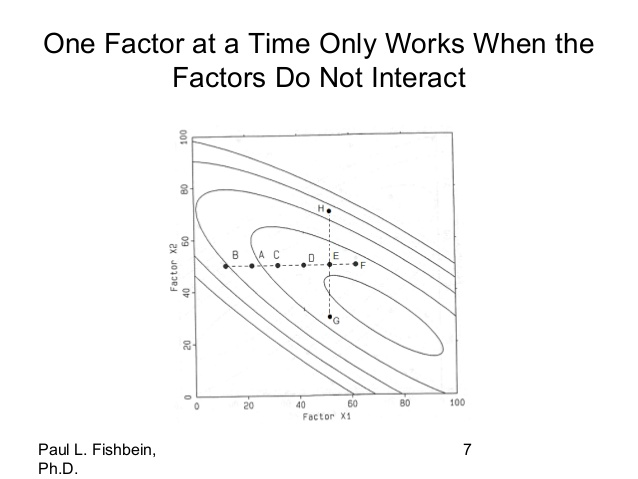
\includegraphics[height=0.3\textheight]{art/optimization-without-statistical-doe-2015-03-23-7-638}
\caption[One-at-a-time optimization]{Optimizing factors, one at a time.\newline \url{http://www.slideshare.net/PaulFishbein/optimization-without-statistical-doe-2015-03-23-46817073}}
\label{fig:one_factor_at_a_time}
\end{figure}




\subsection{Full Factorial Designs}
A \emph{full factorial}, or \emph{complete factorial} design, is one where all factor-level combinations are replicated the same number of times.
The most common of the full-factorial designs is the $2^k$-design where all combinations of $k$ factors with two levels each are tested in each replication.



\subsubsection{$2^k$ design}
Consider two factors denoted $A$ and $B$.
Adopt the effect coding so that we encode their levels by $\set{-1,1}$.
The design matrix of a single run is depicted in Figure~\ref{fig:full_factorial} (top right) along with a visualization of the design (top left).
Allowing $n$ observations per condition, the experiment will include $4n$ observations, which will be randomized between conditions.

\begin{figure}[ht]
\centering
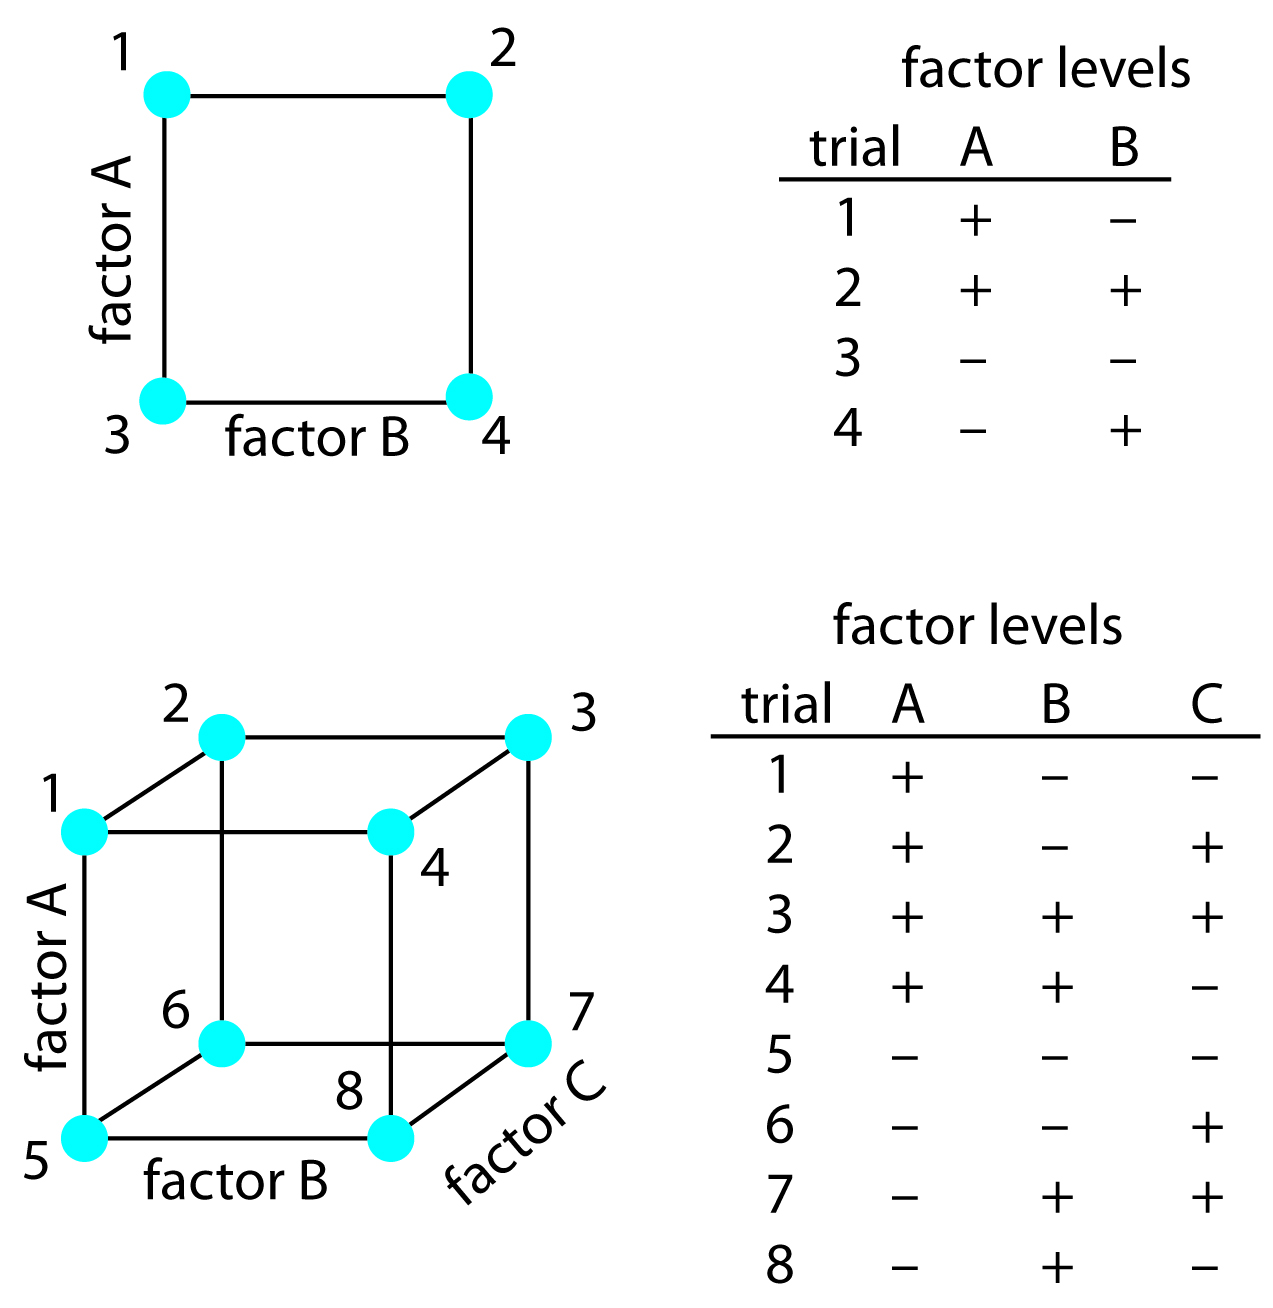
\includegraphics[width=0.7\linewidth, height=0.3\textheight]{art/full_factorial}
\caption[Full Factorial Design]{Full factorial designs: $2^2$ and $2^3$. \newline \url{http://chemwiki.ucdavis.edu/Analytical_Chemistry/Analytical_Chemistry_2.0/14_Developing_a_Standard_Method}}
\label{fig:full_factorial}
\end{figure}
With this $2^2$ design, we may recover several effects:
\begin{description}
\item [Main effect of A] The effect of varying $A$ from $(-)$ to $(+)$\DIFdelbegin \DIFdel{, denoted $\tau^A$}\DIFdelend .
\item [Main effect of B] The effect of varying $B$ from $(-)$ to $(+)$\DIFdelbegin \DIFdel{, denoted $\tau^B$}\DIFdelend .
\item [Main effects and interaction] The effect of varying both $A$ and $B$ from $AB=(--)$ to $AB=(++)$\DIFdelbegin \DIFdel{, , denoted $\tau^{AB}$}\DIFdelend .
\end{description}

We typically denote \DIFaddbegin \DIFadd{the (mean) response for each treatment by the $\mu_{\smiley}$ notation, where $\smiley$ encodes the applied treatment by stating the conditions that were at their $+$ state:
}\DIFaddend \begin{table}[H]
\centering
\begin{tabular}{|c|c|c|c|}
\hline Treatment & A & B & Mean \\ 
\hline 1 & + & - & $\mu_a$ \\ 
\hline 2 & + & + & $\mu_{ab}$ \\ 
\hline 3 & - & - & $\mu_{(1)}$ \\ 
\hline 4 & - & + & $\mu_b$ \\ 
\hline 
\end{tabular} 
\end{table}
\DIFdelbegin \DIFdel{How are these effects related to the mean responses to each treatment?
}\begin{align*}
	\DIFdel{\tau^A }&\DIFdel{:= \frac{1}{4}\left( (\mu_{ab}+\mu_a)- (\mu_{(1)}+\mu_b)\right), }\\
	\DIFdel{\tau^B }&\DIFdel{:= \frac{1}{4}\left( (\mu_{ab}+\mu_b) - (\mu_{(1)}+\mu_a)  \right), }\\
	\DIFdel{\tau^{AB} }&\DIFdel{:= \frac{1}{4}\left( \mu_{ab} +  \mu_{(1)} -  \mu_a - \mu_b \right).	
}\end{align*}
%DIFAUXCMD
\DIFdelend 

\marginnote{Interaction}

Slightly intruding into the realm of data analysis, a visualization of interactions is known as the \emph{interaction plot}, depicted in Figure~\ref{fig:interaction_plot}. 
The upper left panel demonstrates a lack of interaction (think why), while the upper right panel depicts an interaction.
\begin{figure}[ht]
\centering
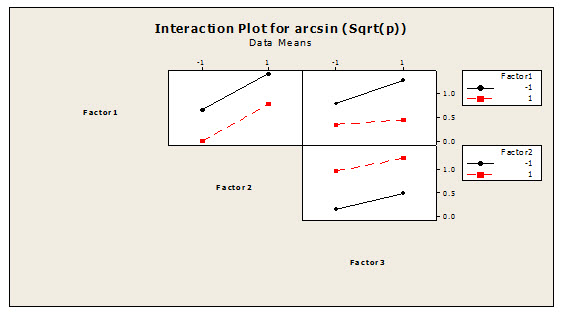
\includegraphics[width=0.3\textheight]{art/attribute_doe_interaction_plot}
\caption[Interactions plot]{Interactions plot. \newline \url{http://blog.minitab.com/blog/statistics-in-the-field/optimizing-attribute-responses-using-design-of-experiments-doe-part-2}}
\label{fig:interaction_plot}
\end{figure}


\begin{remark}[Screening Experiments]
The $2^k$ designs are probably the most popular full factorial designs. 
This may be attributed to the fact that many factors studied really have two levels, but more plausibly, since these are merely \emph{screening} experiments. 
Once non related factors have been screened, the experimenter may proceed from the $2^k$ design to more elaborate ones. 
\end{remark}



\begin{remark}[Intermediate Factor Levels]
In a $2^k$ design, a factor may actually be a continuous controllable input which was restricted to two values for convenience. 
After estimating the effect of the factor, we may want to know what the effect would have been, had we set it on some intermediate level.
It is customary to assume that a main effect acts linearly in-between experimental conditions, yet you should remember that there is nothing in the data to support this.
For a more rigorous approach, see the Response Surface Methodology Section (\ref{sec:response_surface}).
\end{remark}


\begin{remark}[Crossed Treatments]
Both crossover designs and full factorial designs are \emph{crossed} in that all factor combinations are sampled. 
The difference is that in a full-factorial, a factor combination is applied simultaneously to an experiment unit, and in a crossover design, the application is sequential \citep{everitt_cambridge_2010}.
\end{remark}



\subsubsection{$3^k$ Designs}
I think that the name $3^k$ design is rather self explanatory.
Then again, more than $2$ levels are rarely treated as factorial experiments. 
This is because $3$ level factors typically appear when aiming at optimizing the factor combination, for which the \emph{response surface} methodology of Section~\ref{sec:response_surface} is more economical.




\subsection{Fractional Factorial}
Full factorial designs are the simplest designs to setup and interpret. 
A major drawback, are the resources required when $k$ is large. 
This is where the \emph{fractional factorial}, or \emph{partial factorial} designs kick in.
The fundamental idea is to design a full factorial, but skip a couple experimental conditions. If conditions to skip are wisely selected, only information on higher order interactions will be compromised.


\begin{example}[From $2^2$ to $2^{2-1}$]
\label{eg:fractional_factorial}
As a first toy example, we will try to save some time and money by eliminating particular conditions of the $2^2$ design in Figure~\ref{fig:full_factorial}.
As the name may suggest, a $2^{2-1}$ design, has $2$ experimental conditions in each run. 
There are thus $\binom{4}{2}=6$ possible eliminations, which are enumerated in Table~\ref{tab:partial_factorial} along with the extractable information in each elimination.
\begin{table}[ht]
\begin{tabular}{|p{2.5cm}|p{10cm}|}
\hline Elimination &  Problem \\ 
\hline
\hline 1,2 &  No information on $a$. \\ 
\hline 1,3 &  No information on $b$.\\ 
\hline 1,4 &  $a$ aliased with $b$ aliased with $ab$. \\ 
\hline 2,3 &  $a$ aliased with $b$ aliased with $ab$. \\ 
\hline 2,4 &  No information on $b$. \\ 
\hline 3,4 &  No information on $a$.\\ 
\hline 
\end{tabular} 
\caption[Aliasing]{Aliasing in a $2^{2-1}$ design: All possible eliminations from the $2^2$ design that lead to a $2^{2-1}$ design.}
\label{tab:partial_factorial}
\end{table}
\end{example}

The lesson from Example~\ref{eg:fractional_factorial} is that in a fractional factorial our savings in time and money, come at the cost of the information that can be drawn from the experiment.
The idea behind partial factorial experiments, is that by an informed choice of the conditions skipped, we can choose what information to give up. The information lost, is known as the \emph{alias structure}.\marginnote{Alias Structure}

In practice, we will rarely \DIFdelbegin \DIFdel{do the actual elimination }\DIFdelend \DIFaddbegin \DIFadd{go over all the $\binom{2^k}{2^p}$ possible eliminations }\DIFaddend of conditions, but rather revert to pre-selected designs. 
Table~\ref{tab:partial_factorial_ii}, generated with the \rcode{FrF2()} in the \rcode{FrF2} \R package, is an optimal $2^{5-2}$ design.
Using the \rcode{design.info()} function of that same package, we know that the aliasing structure of this design is
$a=bd=ce, b=ad, c=ae, d=ab, e=ac$.
We will not go into the details of how the aliasing structure is computed, but rather refer the reader to \cite{cox_theory_2000}.
\begin{table}[ht]
\centering
\begin{tabular}{rrrrrr}
  \hline
 & A & B & C & D & E \\ 
  \hline
1 & -1 & 1 & -1 & -1 & 1 \\ 
  2 & 1 & -1 & 1 & -1 & 1 \\ 
  3 & -1 & -1 & -1 & 1 & 1 \\ 
  4 & -1 & 1 & 1 & -1 & -1 \\ 
  5 & -1 & -1 & 1 & 1 & -1 \\ 
  6 & 1 & 1 & 1 & 1 & 1 \\ 
  7 & 1 & -1 & -1 & -1 & -1 \\ 
  8 & 1 & 1 & -1 & 1 & -1 \\ 
   \hline
\end{tabular}
\caption[Fractional Factorial Design]{$2^{5-2}$ design.}
\label{tab:partial_factorial_ii}
\end{table}




\begin{definition}[Resolution of a Design]
\DIFdelbegin %DIFDELCMD < \sout{As we have already seen, there are $\binom{2^k}{2^{k-p}}$ possible eliminations that convert a $2^k$ design to a $2^{k-p}$ design.
%DIFDELCMD < We call the \emph{resolution of the design}, the lowest order effect that is aliased. 
%DIFDELCMD < In Table~\ref{tab:partial_factorial_ii}, the resolution is 1, making it a rather unattractive design. 
%DIFDELCMD < Resolutions below 3 typically considered not informative, and above 5, considered wasteful.
%DIFDELCMD < }%%%
\DIFdelend \DIFaddbegin \DIFadd{In previous versions of this text I defined the }\emph{\DIFadd{resolution}} \DIFadd{of a design. 
Since my definition was wrong, you are kindly asked to ignore it.
}\DIFaddend \end{definition}

\begin{tcolorbox}
\paragraph{My mistake!}
The previous definition is plain wrong. 
It is thus removed from the course's syllabus until I update it.
\end{tcolorbox}



\begin{extra}[Coding Theory]
There is a close relationship between design of experiments and coding theory in computer science. 
A possible reference on the matter is \cite{hill_first_1986}, or \cite{hedayat_orthogonal_1999}.
\end{extra}



\subsection{Split Plot Design}
\label{sec:split_plot}
Revisiting our web site layout problem:
We want to block along age and country. 
For each age and country combination (full factorial blocking) we can randomly assign users to site layouts. 
This combination of a factorial design for blocking, is known as a \emph{split plot}, or \emph{split unit} design.
For more on split plots see \cite[Sec.6.4]{cox_theory_2000}.

\DIFaddbegin \subsection{\DIFadd{Summary of Discrete Factors}}
\DIFadd{In this section we dealt with discrete factors, typically taking two possible values.
These appeared for several purposes. 
The most obvious way, was to define treatments: in full factorial, and fractional factorial designs, the treatments are decomposed into their defining factors. 
Decomposing treatments to their factors allowed us to be more economical in our designs (think why?).
Factors were, however, also encountered when reducing variability. 
When used for defining blocks, or groups, we called these non-specific factors simply because all we required for grouping was some vague notion of homogeneity within a block, and not an explicit definition of the factor that defines the blocks. 
}

\DIFadd{In the next section, we extend from discrete factors to continuous factors.
}

\DIFaddend \section{Continuous Factors}
When dealing with \emph{continuous factors}, or \emph{quantitative factors}, we have many more analysis strategies than when dealing with qualitative factors.
No matter the analysis strategy, it is still important of choosing the right factor level combinations to study.

Clearly, we cannot identify nonlinearities when sampling a factor only a two levels.
We may thus opt for a full $3^k$ factorial design to fit a non-linear surface to the data.
The factor encoding would typically be $\{-1,0,1\}$,
A full $3^k$ factorial design may however be needlessly expensive. 
A more common approach in industrial application is the \emph{central composite design}, where a $2^k$ design is augmented with well chosen sampling points. \marginnote{Central Composite Design}
For more details see \cite[Sec.6.6]{cox_theory_2000}


\subsection{Response Surface Methdology}
\label{sec:response_surface}
As the name suggests, \emph{response surface methdology} deals with the estimation of the response surface to the levels of continuous factors.
Response surfaces are typically assume to be (approximately) quadratic, and experimentation typically conducted in stages. First screening factors, then fitting a surface, and finding optimal factor levels.



\subsection{Taguchi Methods}
\emph{Taguchi methods} is a collective name for the philosophy, design, and analysis methods in industrial applications promoted by Genichi Taguchi in 1970's Japan.
Focusing on the design principles, we may note the following particularities of Taguchi's method:
\begin{enumerate}
\item Achieving low variability is more challenging then achieving a target value. 
\item Factors which can be controlled in a lab, but not in production, are deliberately varied. Typically with split plot  designs (\ref{sec:split_plot}).
\item Systematic use of latin hypercubes to study main effects and two-way interactions. Particularly \emph{Plackett–Burman designs}.\marginnote{Plackett Burman Design}
\item Log variability ($\log s$) is often used as the response.
\end{enumerate}





\DIFdelbegin \subsection{\DIFdel{Optimal Designs}}
%DIFAUXCMD
\addtocounter{subsection}{-1}%DIFAUXCMD
\DIFdelend \DIFaddbegin \section{\DIFadd{Optimal Designs}}
\DIFaddend 


Our discussion until now has been informal with respect to the desirable qualities of a design. 
We used the idea of ``balance'' and ``orthogonality'' to avoid bias and unwelcome variability.
In this section, we try to formalize the notion of a ``good design''.
We start with some motivating examples.

\begin{example}[Design for linear regression]
\label{eg:design_linear}
Figure~\ref{fig:design_linear} demonstrates the effect of the different location of the sampling points ($x$) on the quality of the estimated regression line, in a \textbf{linear} model.
As the figure depicts, and intuition suggests, it is preferable to spread the sampling points as far as possible.
\begin{figure}[ht]
\centering
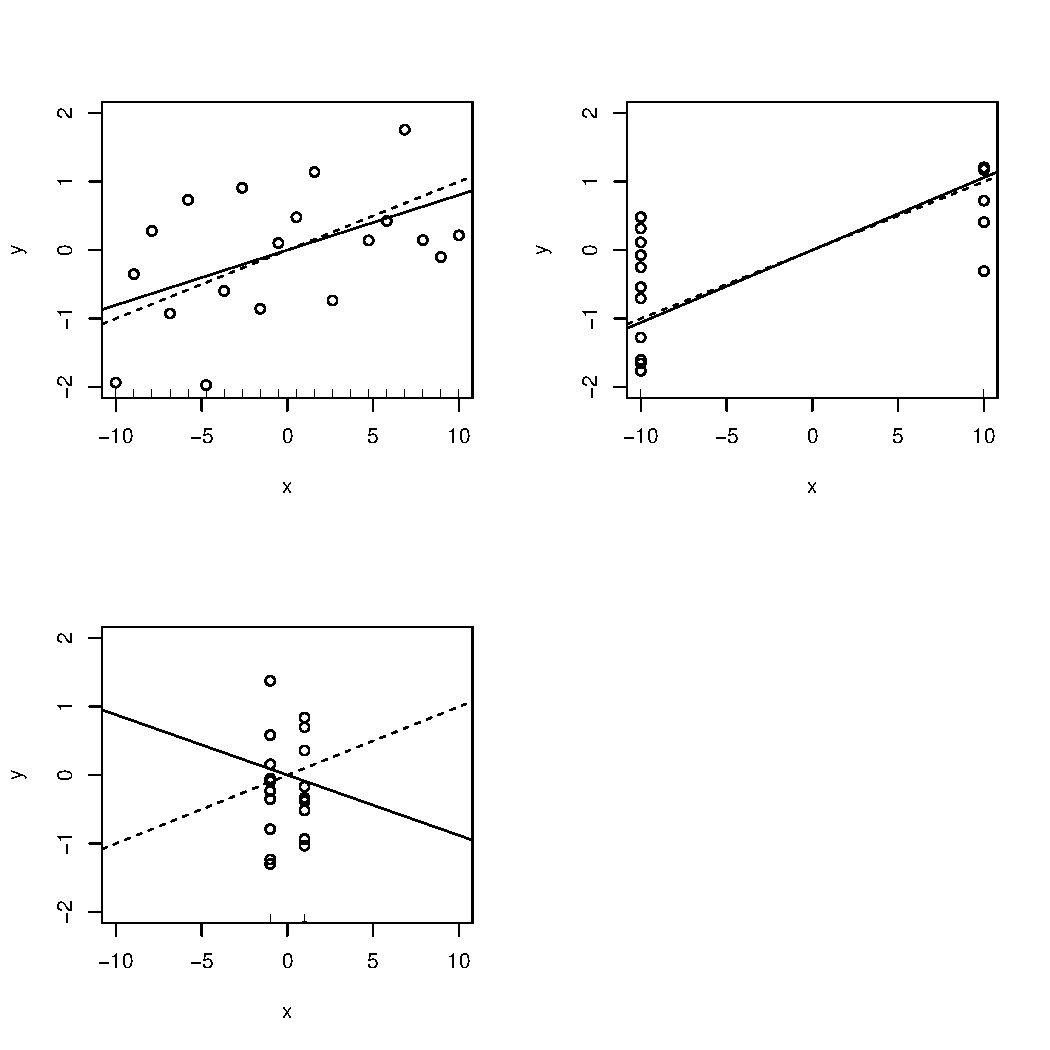
\includegraphics[height=0.3\textheight]{art/linear}
\caption[Design for Linear Models]{Design for linear regression. Different panels show different designs. True function as a dashed line. Estimated function as a full line.}
\label{fig:design_linear}
\end{figure}
\end{example}





\begin{example}[Design for non linear regression]
\label{eg:design_non_linear}
Figure~\ref{fig:design_nonlinear} demonstrates the effect of the different location of the sampling points ($x$) on the quality of the estimated regression line, in a \textbf{nonlinear} model.
It may seems that unlike the linear case (Example~\ref{eg:design_linear}) optimality is achieved in some intermediate spread of the $x$s.
\begin{figure}[ht]
\centering
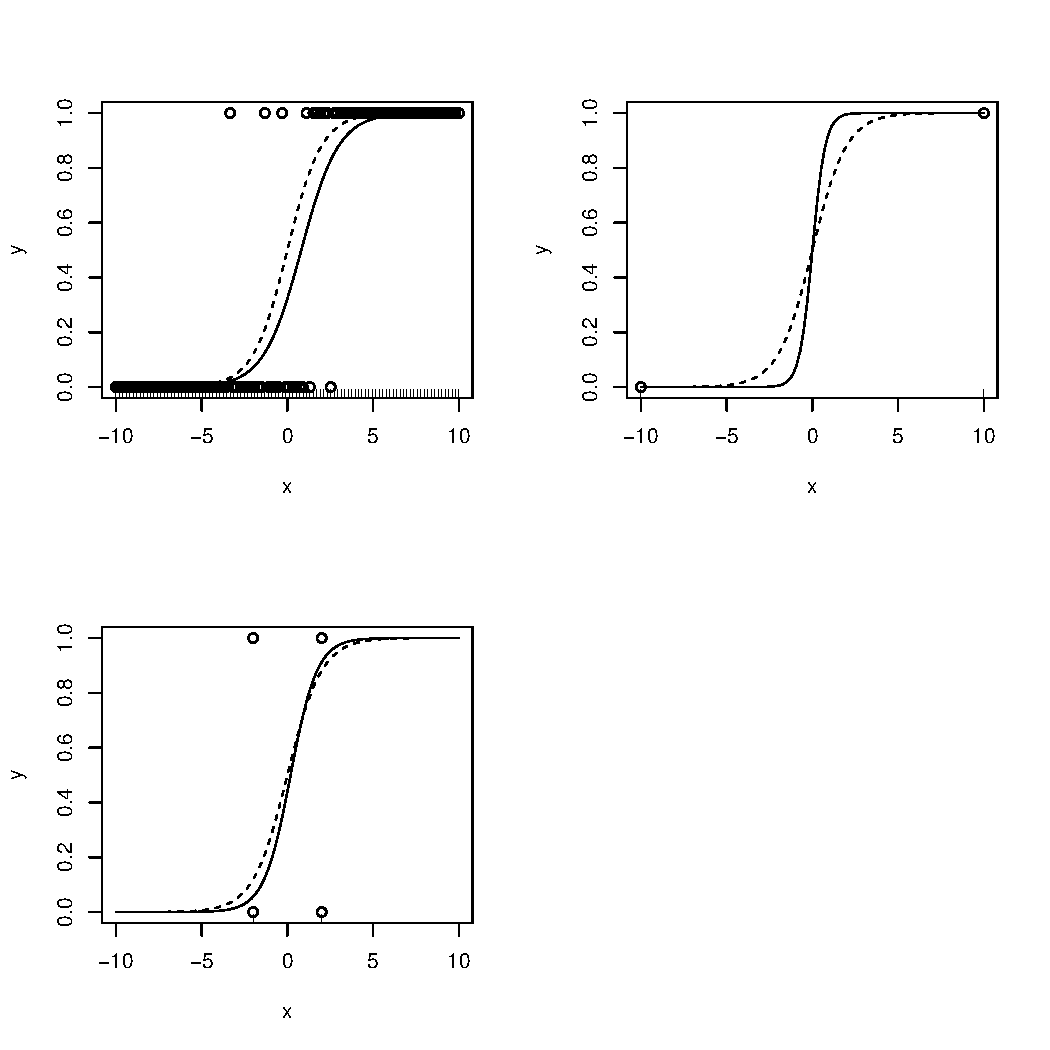
\includegraphics[height=0.3\textheight]{art/nonlinear}
\caption[Design for Non Linear Models]{Design for non linear regression. Different panels show different designs. True function as a dashed line. Estimated function as a full line.}
\label{fig:design_nonlinear}
\end{figure}
\end{example}





Now for some facts, supported by the previous examples:
\begin{enumerate}
\item The idea of ``balancing'' as a design criterion is very useful with discrete factors, but limited with continuous factors. 
\item The optimal design may depend on the unknown generative model. Luckily, for linear models, this is not the case, and an optimal design will be so for all values of the generative parameter.
\end{enumerate}



\subsection{Space Filling Design}
\label{sec:space_filling}
The most natural of designs, which is particularly suitable when we have no a-priori assumption on the functional relation ($f(x)$) between the (continuous) factors and the response, is known as a \emph{space filling design}.
As the name suggests, in a space filling design we aim at filling the factor space. Lacking any a-priori information, the filling will typically be as uniform as possible. 
We note however, that once information on $f(x)$ is made available, then a space filling design is typically sub optimal (see Example~\ref{eg:design_linear}).


\begin{extra}[Space Filling and Hashing]
If you are familiar with the idea of \emph{hashing functions}, then you may see the similarity between space filling and the \emph{uniformity} property of hash functions. 
For a more rigorous discussion, see \cite{hill_first_1986}.
\end{extra}



\subsection{Covariance Optimality}
We have already noted the the optimality of the design depends on the data generating process.
In this section it is made obvious that optimality will also depend on the analysis method we choose.

When estimating the effect of a single continuous factor, we would like a design that gives us the most information per observation on some effect $\beta$. 
This is the same as minimizing the variance of the estimator, $\min \{Var[\hat{\beta}]\}$, with respect to the design.
In the case of linear regression with a single coefficient we know that 
\begin{align}
	Var[\hat{\beta}] &= \frac{\sigma^2_\varepsilon}{\sum_{i=1}^{n}(x_i-\bar{x})^2}.
\end{align}
Minimizing $Var[\hat{\beta}]$ is thus the same as spreading the $x$'s as far as possible, in accordance with the intuition from Example~\ref{eg:design_linear}.
Now recall that in a multivariate linear regression problem with an $n \times p$ design matrix, then 
\begin{align}
	Var[\hat{\beta}] &= \sigma^2_\varepsilon (X'X)^{-1}.
\end{align}
In this multivariate case, there may be several notions of ``maximal spread''. 
Denoting $M:= (X'X)^{-1}$, we can define:
\begin{definition}[A-Optimality]
	A design is said to be \emph{A optimal} if it minimizes the average univariate variance.
	Formally: $\min \set{\Tr(M)}$.
\end{definition}
A-optimality does not account for covariances. 
In an extreme scenario, if we have several copies of the same variable, the more copies we have, the more importance that variable will be given by A-optimality.
The most popular optimality criterion is known as \emph{D-optimality}, and does not suffer from this phenomenon.
\begin{definition}[D-Optimality]
	A design is said to be \emph{D optimal} if it minimizes the volume of the confidence region for $\beta$. 
	Formally: $\min \set{\det(M)}$.
\end{definition}

Both A-optimality and D-optimality implicitly target linear models, such as in Example~\ref{eg:design_linear}, because they aim at spreading the $x$'s. From Example~\ref{eg:design_non_linear} we know this to be sub-optimal doe non-linear designs. 
For non-linear designs, one may opt for space filing designs (\ref{sec:space_filling}), or consult \cite{pukelsheim_optimal_1993}. 



\begin{extra}[Other Optimality Criteria]
There are as many optimality criteria as there are matrix norms. For a more detailed review, see \cite{wikipedia_optimal_2015}.
For a mathematical rigorous, and through treatment, see \cite{pukelsheim_optimal_1993}.
\end{extra}







\section{Sequential Designs}
\label{sec:sequantial}

Consider a clinical trial with a treatment and control group.
Now assume the medicine being tested is a miracle cure with immediate improvement. 
Do we really need to keep administering placebos to the control group, just because that was the initial experimental design?
This is where sequential designs come in.
Interestingly, the initial application of a sequential design was not in drug testing, but rather in a military context \citep{wald_sequential_1945}.

The problem with sequential testing, is the \emph{type-I error inflation}, which is simply a \emph{multiplicity problem}. \marginnote{Multiplicity}
To see this, think about an endless sequential experiment. Also assume the null hypothesis is true. 
Because of consistency, then a regular (non sequential) experiment will not reject $H_0$?
But if the test is sequential, the type-I error of endlessly many tests at level $\alpha$ each, will certainly be making more than $\alpha$ mistakes (unless dependence is perfect).

In it simplest version, a sequential design allows early stopping for rejection of the null, or for futility (non-rejection). 
In more elaborate schemes then not only is early stopping allowed, but also the redesign of the experiment. 
This is known as \emph{adaptive design}. The crux, as usual, is not inflating the type-I error, or introducing bias, by redesigning.\marginnote{Adaptive Design}

\begin{extra}[Active Learning]
In the machine learning literature, the idea of adaptive design of experiments is known as \emph{active learning}, where the emphasis is less on adaptive-testing, but rather on adaptive-estimation.
\end{extra}




\subsection{Pooled Designs}
\emph{Pooled designs}, \aka as \emph{group testing} appears when it is cheaper to measure the response for a group of experimental units simultaneously, rather then for each single one. 
It originated in the context of identifying soldiers with syphilis in WWII. It was the Harvard Economist Robert Dorfman that suggested \cite{dorfman_detection_1943} that one may mix blood samples from several soldiers and then repeat the same in the subgroups that show the presence of syphilis. 
The method became immensely popular in the DNA analysis age, where technology allows biologists to test for the presence of particular protein in a sample from a group of cells (e.g. a blood sample). 

Pooled designs broadly classify into two classes: 
\begin{description}
\item [Adaptive group testing] Where the groupings, and the groups to be tested depend on the previous results in the same experiment (see also \emph{adaptive designs}).
\item [Non-adaptive group testing] Where the experiment consists of sequential group tests, but the design is fixed independently of the experimental results. 
\end{description}


\begin{extra}[Bloom filters]
If you are familiar with data structures and particularly \emph{Bloom Filters}, then you will probably note that a Bloom filter is a data structure that groups objects in a way that facilitates lookup using group testing. 
\end{extra}



\section{$A\backslash B$ Testing}
Our web-site optimization example is interesting not only because it accommodates so many DOE practices, but it is also a practical problem of great interest.
For historical reasons, the experimentation with several web-site layouts is not called a factorial experiment (which it is), but rather an \emph{$A\backslash B$-test}.

Some particular characteristics of $A\backslash B$ testing include:
\begin{enumerate}
\item Users come by the millions. Sample size is rarely an issue, so that avoiding bias is more important than avoiding variability.
\item Browser cookies, or login details define blocks. Technology permits to optimize the size for each block separately. If blocking is to very specific subgroups (female users, running Linux, that purchased on Amazon, etc.), then sample size, and thus variability, may become an issue again.
\item Sites have many layout parameters (locations, colours, sizes,...). Studying all these combinations may result on a formidable task (full factorial?!?).
\end{enumerate}




\section{Computer Experiments}
\begin{example}[Designing Wings]
\label{eg:wings}
Consider the problem of designing an air-craft's wing.
We would like to know how the wing's attributes, i.e., factors, govern its lift.
We could obviously conduct real-life experiments by varying the wing's attributes, building the wing, flying the air-plane, and recording results. 
Needless to say how expensive this process is.
It is much more reasonable to program the differential equations that govern the lift to a computer, fix several factors values, and solve the equations.
This is what \emph{computer experiments} are all about. 
\end{example}


The wind design example (\ref{eg:wings}) demonstrates the following points:
\begin{enumerate}
\item Computer experiments are essentially numerical solutions to complicated systems of equations.
\item Because solutions take a lot of time, only a small finite set of factor levels may be evaluated. 
\item The ``response'' to each treatment, is deterministic. 
\item The problem of interest is in reconstructing the response at non measured factor levels, so that optimal values may be identified. 
\end{enumerate}
It is thus not uncommon to call upon DOE theory for choosing the factor combinations to be experimented with. Space filling designs (Sec.~\ref{sec:space_filling}) being a particularly prevalent choice. 
The analysis of computer experiment is very different than real-life experiment since we have no noise component. 
See \cite{sacks_design_1989} or \cite{santner_design_2013} for further details. 



\section{Bibliographic Notes}
For an overview of DOE see \cite{cox_theory_2000}, \cite{mason_statistical_2003}, \cite{everitt_cambridge_2010}. 
Another nice and freely available resource is a Penn State course on the topic\footnote{\url{https://onlinecourses.science.psu.edu/stat503/node/1}}. 
Some seminal references in the field include \cite{fisher_design_1960} and \cite{box_statistics_1978}.
For causal inference in non-designed experiments see \cite{rosenbaum_observational_2002}. 
For optimal designs see \cite{pukelsheim_optimal_1993}.
For analysis of data: linear models, ANOVA, etc.\ there are endlessly many books. This author's recommendations include \cite{hocking_analysis_1985}, \cite{greene_econometric_2003}. 
For the relation between factorial designs and coding theory in computer science, see \cite{hill_first_1986}. 
For design and analysis of computer experiments, see \cite{sacks_design_1989} or \cite{santner_design_2013}.

\chapter{Acceptance Sampling}
\chaptermark{Acceptance}


We can improve quality (read- conformance to specification) by introducing an inspection stage in our process.
Clearly, a full inspection is time consuming. 
It may also be destructive (you don't want to re-package ice-cream after checking its texture \dots).
No-inspection may be appropriate if you don't particularly care about your brand, or if production has very high capability indices.
A reasonable, intermediate approach, is a partial random inspection, known as \emph{acceptance sampling}.
As the name suggests, in acceptance sampling, one samples, then checks, then accepts (or not).

Acceptance sampling can be seen as a control chart monitoring that triggers active intervention in the production. As such ,it is a crude type of \emph{engineering control} (Sec.~\ref{sec:terminology_statistical}).
The intervention is obvious. The monitoring is based on some continuous (variable) or discrete (attribute) of a sample of units from a \emph{batch}, \aka, a \emph{lot}.
Seen as a feedback control, it is not surprising that when designing an acceptance sampling scheme, we have similar decisions as when designing a control chart:
\begin{enumerate}
\item What is a batch? Just like choosing the sampling frequency in a Shewart chart. 
We would like homogenous batches, i.e., with low inner variability. A box, a shipment, a day's production, are typical batches. 
\item Within batch sampling scheme: just like rational grouping in Shewart chart. Typical approaches include \emph{single sampling plans}, \emph{double}, \emph{multiple}, and \emph{sequential sampling plans}.
This can be seen as the design of an experiment to be performed on each batch.
\item How many units? Just like choosing the sample size in a Shewart chart.
\item Decision cutoff: Just like setting control limits in a Shewart chart. 
\end{enumerate}
We can readily see that the design of an acceptance sampling scheme is very similar to the design of a control chart. 
We may construct an full blown economical optimization problem to design the sampling, as we did in Section~\ref{sec:economical_considerations}. Just like control charts, however, it is more common to design sampling schemes using ``first-order'' power considerations. 
For this reason, the \emph{power function} will play a crucial role.

\section{Acceptance Sampling Terminology}
Adapted from \cite{natrella_nist/sematech_2010}.
\begin{description}
\item [LASP] A \emph{lot acceptance sampling plan}, ultimately, a statistical test at the end of which we either accept a batch. In this text we typically use the \emph{batch acceptance sampling scheme} for the same purpose. 
\item [AQL] The \emph{acceptable quality level}, or \emph{acceptable quality limit}, is the highest proportion of defects acceptable to the producer. 
\item [LTPD] The \emph{lot tolerance percent defective} is the highest proportion of defects acceptable to the consumer. Clearly, $AQL<LTPD$. LTPD is also known as \emph{rejectable quality level} (RQL), and \emph{ limiting quality level} (LQL). 
\item [OC Curve] The \emph{operating characteristic curve} is the power function of an LSAP.
\item [Type-A and Type-B OC Curves] A \emph{Type-A OC curve} is one computed assuming sampling from batches is done without replacement. Conversely, a \emph{Type-B OC curve} is computed assuming sampling with replacement.
\item [Producer's Risk] The \emph{producer's risk} is throwing away good batches. Formally, this is the probability of rejecting a batch with less than AQL defects. We consider there type-I errors.
\item [Consumer's Risk] The \emph{consumer's risk} is accepting bad batches. Formally, this is the probability of accepting a batch with more than LTPD defects. We consider there type-II errors.
\item [Rectifying Inspection] An LASP where lots are not rejected but rather rectified. 
\end{description}



\section{Single Sampling Scheme}
In the simplest LASP we base our decisions on a single random sample from each batch.
This obviously facilitates the statistical analysis of the properties of this LASP.

\subsubsection{Type-B Power Function}

When sampling $n$ units from a batch with a proportion of $p$ defects, then the number of defects $\x \sim Binom(n,p)$.
If we reject a batch when more than $c$ defects are found, then the power function of a type-B LASP is given by
\begin{align}
\label{eq:power_accpet}
	\pi_{n,c}(p)=P(\x \geq c)= \sum_{k=c}^n \binom{n}{k} p^k (1-p)^{1-k} .
\end{align}
Eq.(\ref{eq:power_accpet}) may be evaluated manually, or with the \rcode{pbinom()} \R function. 

Just like any other hypothesis test, it is common practice to set $n,c$ so that control both the consumer's risk ($\beta_{n,c}=1-\pi_{n,c}$) and the producer's risk ($\alpha_{n,c}$).
By adopting a the hypothesis testing philosophy, we solve $n,c$ so that 
\begin{align}
\label{eq:power_acceptance}
 \min \set{n : \pi_{n,c}\geq \pi_0 \quad and \quad \alpha_{n,c}\leq \alpha_0 }.
\end{align}
For relating the LASP terminology to this problem, we need to observe that $$\alpha_{n,c}=\pi_{n,c}(p=AQL)$$ and $$\pi_{n,c}=\pi_{n,c}(p=LTPD).$$
For a producer who does not want to reject batches where $AQL=10\%$ defects, with more than $\alpha_0=10\%$; 
and a consumer who does not want to accept batches where $LTPD=30\%$, with less than $\pi_0=80\%$, 
we have that their LASP would take $n=33$ samples, and reject a batch whenever the $\x>4$, when $n=21$.
\begin{remark}[Approximate Power Calculations]
The problem to solve in Eq.(\ref{eq:power_acceptance}) requires some non trivial iterations because of the discrete nature.
It is quite more convenient to replace the exact form of Eq.(\ref{eq:power_accpet}) with a normal approximation, so that Eq.(\ref{eq:power_acceptance}) has a closed form solution. 
\end{remark}



\subsubsection{Type-A Power Function}
It is quite wired that we would sample with replacement from a batch.
It is quite more probable that we used the replacement assumption, only as an approximation because $n$ is small compared to the batch size $N$. 
If this is not the case, the binomial distribution in Eq.(\ref{eq:power_accpet}) should be replaced with the Hypergeometric distribution. 
For all practical purposes, this means using the \rcode{phyper()} \R function, instead of \rcode{pbinom()}.



\subsection{Double Sampling Scheme}
In a double sampling scheme, we first example $n_1$ units. 
We may then decide to accept, reject, or sample another $n_2$ units. 
After those $n_2$ samples, we can accept or reject. 
The idea of a power function remains the same, even if calculations are slightly more cumbersome.
Here is our our policy:
For $x_1$ computed on the first $n_1$ samples:
If $x_1  < a_1$ then accept the batch;
If $x_1 \geq  c_1$ then reject the batch;
Otherwise, compute $x_2$ with $n_1+n_2$ samples.
If $x_2 < a_2$ accept the batch;
If $x_2 \geq c_2$ then reject the batch.

For brevity, we denote all the design parameters of the scheme by $\gamma:= (n_1,n_2,c_1,c_2,a_1,a_2)$. 
The power function of such a scheme would thus be:
\begin{align}
	\pi_\gamma &:= P(\set{\x_1 \geq c_1} \union \set{\x_1 \in [a_1,c_1], \x_2 \geq c_2}) \\
	&= P(\x_1 \geq c_1) + \sum_{k=a_1}^{c_1} P(\x_1 =k, \x_2-\x_1 \geq c_2-k) \\
		&= P(\x_1 \geq c_1) + \sum_{k=a_1}^{c_1} P(\x_1 =k) P(\x_2-\x_1 \geq c_2-k).
\end{align}
We may now use the fact that $\x_1 \sim Binom(n_1,p)$ and that $\x_2-\x_1 \sim Binom(n_2,p)$, and quickly compute the power in \R.

\begin{remark}[Redundancy]
Unlike the single stage LASP, where we have two equations with two variables, in the two-stage case there are many $\gamma$ configurations that will achieve given consumer and producer risks ($\alpha_0,\pi_0$).
The choice of the particular configuration should depend on the type of signal we expect. 
For quick detection of strong signal (large $p$), choose small $n_1$. 
For sensitive detection of subtle signal, choose large $n_1$. 
\end{remark}

\begin{remark}[No Free Lunch]
While it may seem that a two stage LASP is always better than a single stage LASP, this is not the case.
To see why, consider a weak signal ($p$ close to AQL). We may need all $n_1+n_2$ samples to get decent power. The first stage then add nothing except logistic complications.
\end{remark}


\section{Sequential Scheme}
At this point you should be thinking: why only two stages? 
Clearly we may reject or accept a sample as each unit comes in.
This is exactly what Sequential LASPs are all about.
We will not give the details, except the observation that this is merely a type of sequential experiment as described in Section~\ref{sec:sequantial}.




\section{Bibliographic Notes}
[TODO] 


\chapter{Reliability Analysis}
\chaptermark{Reliability}

The attempt to define the difference between \emph{reliability} and \emph{quality} will certainly fail given the intentional ambiguity in our definition of \emph{quality} (Chapter~\ref{sec:introduction}).
For our purposes, however, this terminological matter will not matter, since we will simply define reliability analysis to be the analysis of the \emph{time} to \emph{failure}.
We will also assume that ``time'' and ``failure'' are well defined and agreed upon.

We intuitively understand ``more reliable'' to mean ``lasts longer''. 
We should also consider, however, the case of a product that is designed to fail after some time, thus forcing the consumer to buy a new one. 
Some may say that a major hi-tech company named after a fruit employs this practice. 
Be it true or not, I hope we can agree that good knowledge of your product's life expectancy is a desirable. 

Reliability analysis involves the study of a probabilistic property of our product- its \emph{survival}.
Any probabilistic model will require calibration to reality via data. 
This chapter thus introduces both the probability calculus typically used for reliability analysis, and some statistical considerations involved when calibrating these models.



\section{Probabilistic Analysis}




\subsection{A Static View}

Let $\x_j \in \set{0,1}, j=1,\dots,p$ denote the state of the $j$'th component of a system, and $x=(x_1,\dots,x_p)$.

\begin{definition}[Structure Function]
The \emph{structure function}, $\struct=\struct(x):x \mapsto \set{0,1}$, is an indicator function of the state of the system. A failure indicated by $0$. 
\end{definition}

\begin{remark}[$\Phi$]
We apologize to the reader for using $\Phi$ to denote both the $\gauss{0,1}$ CDF, and the structure function.
We do so to stay in accordance with reliability literature, and since no collisions are created in this chapter by doing so.
\end{remark}

\begin{definition}[Series System]
A \emph{series system}, or \emph{serial system}, is one where all components need to function for the system to function: $$\struct(x)=\prod_{j=1}^{p}x_j.$$
\end{definition}
A reliability diagram of a series system is given in Figure~\ref{fig:series_system}.
\begin{figure}[ht]
\centering
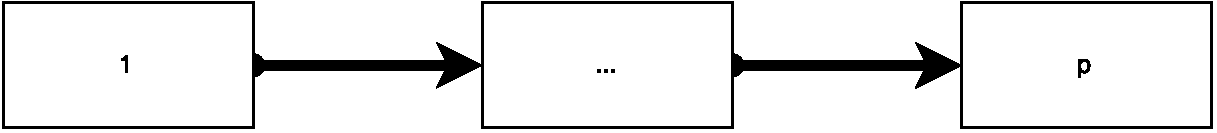
\includegraphics[width=0.5\linewidth]{art/series_system}
\caption{Series system.}
\label{fig:series_system}
\end{figure}


\begin{definition}[Parallel System]
A \emph{parallel system} is one where all components need to fail for the system to fail:
$$\struct(x)=1-\prod_{j=1}^{p} (1-x_j)= \coprod_{j=1}^p x_j.$$
\end{definition}
A reliability diagram of a parallel system is given in Figure~\ref{fig:parallel_system}.
\begin{figure}[ht]
\centering
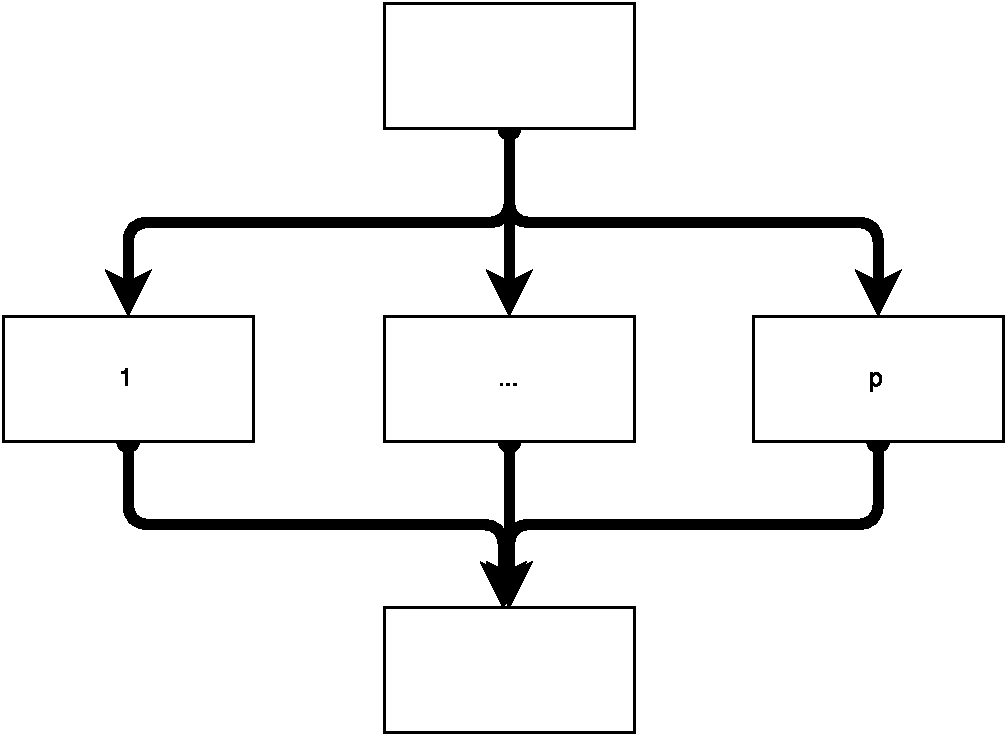
\includegraphics[width=0.5\linewidth]{art/parallel_system}
\caption{Parallel system.}
\label{fig:parallel_system}
\end{figure}





\begin{definition}[k-out-of-p System]
A \emph{k-out-of-p} system is one where at least $k$ components need to function for the system to function:
$$\struct(x)=\indicator{\sum_{j=1}^{p} x_j \geq k}.$$
\end{definition}
A reliability diagram of a k-out-of-p system is not provided, since it is not very friendly. Try thinking of a 2-out-of-3 system to see why.




\begin{tcolorbox}
\paragraph{My mistake!}
The previous definition is different than the one I gave in class. 
I initially defined it via failing components, while now it is defined via functioning components.
Please note this when comparing your notes to mine.
\end{tcolorbox}




\begin{definition}[Monotone System]
A system is said to be \emph{monotone} if $\struct(x_1,\dots,x_p)$ is non decreasing in all components.
\end{definition}
The definition of monotonicity captures the idea that you cannot improve a system's state by breaking components.
This seems rather natural (I am still looking for a counter example).






\begin{definition}[Reliability]
We define the \emph{reliabity of component $j$} to be $$p_j:= P(\x_j=1),$$ 
and  the \emph{reliability of the system} 
$$ S_\struct = S_{\struct(x)}:=P(\struct(x)=1).$$
\end{definition}


\begin{example}[Reliability of a series system]
For $\Phi(x)$ a series system, assuming independent components, we have
$$ S_\struct= \prod_{j=1}^{p} p_j.$$
\end{example}


\begin{example}[Reliability of a parallel system]
For $\Phi(x)$ a parallel system, assuming independent components, we have
$$ S_\struct= 1-\prod_{j=1}^{p} (1-p_j)= \coprod_{j=1}^p p_j. $$
\end{example}


\begin{example}[Reliability of a k-out-of-p system]
For $\Phi(x)$ a k-out-of-p system, assuming independent components with equal reliability ($p_i=p_0$), we have
$$ S_\struct= \sum_{i=k}^{p} \binom{p}{i} p_0^i (1-p_0)^{p-i} .$$
\end{example}



\subsubsection{State enumeration method}
To compute the reliability of more complex structures, the brute-force approach is the \emph{state enumeration method}. 
This method simply relies on summation of the probabilities of the states for which the system functions.
$$ S_\struct= \sum_{x} \Phi(x) P(\x=x).$$


\subsubsection{Factoring method}
The \emph{factoring method}, \aka \emph{pivot-decomposition method}, relies on two ingredients: 
(a) conditioning on the state of some components greatly simplifies the structure, and
(b) the total probability argument.
Combining the two we have:
$$ S_\struct= p_j  S_{\struct|x_j=1} + (1-p_j) S_{\struct|x_j=0}   ,$$
where $S_{\struct|x_j=1}$ denotes the reliability of the structure $\Phi$ conditional on $x_j=1$.
The following example demonstrates the power of the factoring method.

\begin{example}[Bridge Structure]
\label{eg:bridge}
Consider structure in Figure~\ref{fig:bridge}.
To compute the reliability, we will call upon the factoring method while conditioning on the state of component $3$:
$$ S_\struct= p_3  S_{\struct|x_3=1} + (1-p_3) S_{\struct|x_3=0}   .$$
Now note that when $x_3=1$ then we have a series structure of parallel structures, while when $x_3=0$ we have a parallel structure of series structures.:
\begin{align*}
	S_{\struct|x_3=1} &= (p_1 \coprod p_2) (p_4 \coprod p_5),\\
	S_{\struct|x_3=0} &=  p_1 p_4 \coprod p_2 p_5,
\end{align*}
so that 
$$ 	
	S_\struct = p_3  (p_1 \coprod p_2) (p_4 \coprod p_5) + (1-p_3) (p_1 p_4 \coprod p_2 p_5).
$$
\begin{figure}[ht]
\centering
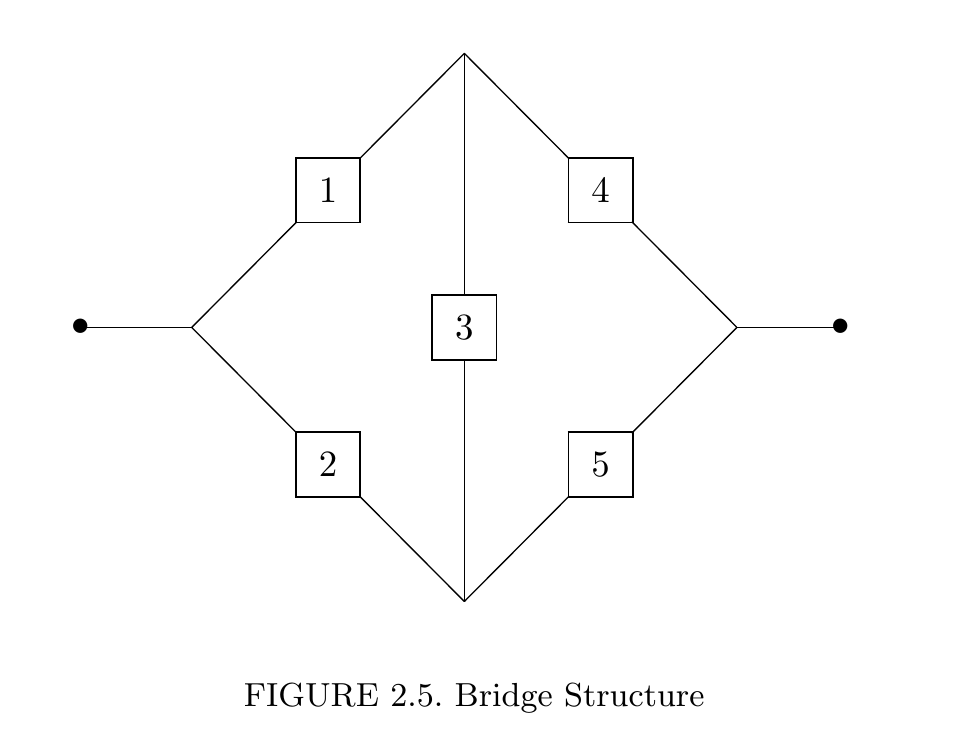
\includegraphics[width=0.5\linewidth]{art/bridge}
\caption{Structure of a bridge system. Source: \cite[Fig.2.5]{aven_stochastic_1999}}
\label{fig:bridge}
\end{figure}
\end{example}
Example~\ref{eg:bridge} demonstrates a single application of the factoring method. Clearly, it can be applied recursively for more complicated systems.

The example also demonstrates a more general principle. Namely, that redundancy is preferable at the component level, and not at the system's level.
Put differently- when designing a backup, and the resources allow a fill copy of the original system, we are better of by designing a component-wise backup, than a single backup system.
Put formally:
\begin{theorem}[Component-wise redundancy]
For a monotone structure $\Phi$, 
\begin{align}
	S_{\struct(x \coprod y)} \geq S_{\struct(x)} \coprod S_{\struct(y)}
\end{align}
where $x \coprod y$ denotes a component-wise backup: $(x_1 \coprod y_1,\dots,x_p \coprod y_p)$.
\end{theorem}



\begin{extra}[Reliability analysis of complex systems]
Except for simple systems, of the type we presented, the computation of the reliability of a complex system may be a formidable task. 
For complicated real-life systems, \emph{min-cut--max-flow} algorithms, or \emph{inclusion-exclusion} type algorithms are employed. 
For more details, see \cite{aven_stochastic_1999}.
\end{extra}









\subsubsection{Reliability Importance Measures}
\begin{quotation}
The Strength Of The Chain Is In The Weakest Link.
\end{quotation}
This is obviously a profound observation in reliability analysis.
In order to identify the weakest link we require some measure of reliability importance.


\begin{definition}[Improvement potential]
The \emph{improvement potential} is defined as the change in a system's reliability, if we could force a component to function indefinitely.
Formally, we denote $\Phi^{(j)}$ to be a system where component $j$ cannot fail. 
We then define the improvement potential with respect to component $j$ to be 
\begin{align}
	I_j :=S_{\Phi^{(j)}}-S_{\Phi}.
\end{align}
\end{definition}



\begin{definition}[Birenbaum's measure]
\emph{Birenbaum's measure} is defined as the change in a system's reliability, if we infinitesimally improve the reliability of component $j$.
Formally 
\begin{align}
	I_j: =\frac{\partial}{\partial p_j} S_{\Phi}.
\end{align}
\end{definition}


Clearly any such importance measure, once computed, may serve to decide which component should be treated to improve reliability.







\subsection{A Time Dynamic View}
The reliability of each component ($p_j$), typically changes in time, and so does the reliability of the whole system.
In the following, $\T$ will typically stand for the time to malfunction. It is thus assumed to be \textbf{continuous} and \textbf{non-negative}.


\begin{definition}[CDF]
The cumulative distribution function (CDF) of a random variable $\T$ at a point $t$  is given by
\begin{align}
	\cdf{\T}{t}:= P(\T<t).
\end{align}
\end{definition}

\begin{definition}[PDF]
The probability density function (PDF) of a continuous random variable $\T$ at a point $t$ is given by 
\begin{align}
	\pdf{\T}{t}:= \frac{\partial}{\partial t}\cdf{\T}{t}.
\end{align}
\end{definition}


\begin{definition}[Survival Function]
The survival function of a random variable $\T$ at a point $t$ is given by 
\begin{align}
	\survive{\T}{t}:= P(\T>t)=1-\cdf{\T}{t}.
\end{align}
\end{definition}
By definition, it follows that if $\T_j$ is the time to failure of component $j$, then $p_j(t)=\survive{\T_j}{t}$.
If $\T_\struct$ is the time to failure of a system $\Phi$, then we may write $S_\struct(t)=\survive{\T_\struct}{t}$.


\begin{example}[Survival of a series system]
For a series system $\struct$, the reliability of the system at time $t$ is given by $$\survive{\Phi}{t}=\prod_{j=1}^{p} p_j(t).$$
\end{example}


\begin{example}[Survival of a parallel system]
For a parallel system $\struct$, the reliability of the system at time $t$ is given by $$\survive{\Phi}{t}=1- \prod_{j=1}^{p} (1-p_j(t))= \coprod_{j=1}^p p_j(t).$$
\end{example}





Another way to present a distribution, no less informative than the previous ones, is by the \emph{hazard function}, which is the ``probability of surviving just another instant''.
\begin{definition}[Failure Rate]
The \emph{hazard function}, or \emph{failure rate}, of a random variable $\T$ at a point $t$ is given by \marginnote{Hazard Function}
\begin{align}
	\hazard{\T}{t} &:= \lim_{dt\to 0}\frac{P( \T \in [t,t+dt)|\T \geq t )}{dt} \label{eq:hazard}\\
	&= \frac{\pdf{\T}{t}}{\survive{\T}{t}} \\
	&= - \frac{\partial}{\partial t}\log \survive{\T}{t} . \label{eq:survival_to_hazard}
\end{align}
\end{definition}





\begin{definition}[Cumulative Risk]
The \emph{cumulative hazard}, \aka the \emph{cumulative risk}, of a random variable $\T$ at a point $t$ is given by \marginnote{Cumulative Hazrd}
\begin{align}
	\cuhazard{\T}{t} &:= \int_{0}^{t}\hazard{\T}{t} \\
	\Rightarrow \survive{\T}{t} &= \exp(-\cuhazard{\T}{t}). \label{eq:cumhazrd}
\end{align}
\end{definition}
Eq.(\ref{eq:cumhazrd}) readily shows that a distribution is well defined by its hazards.



\begin{theorem}[Failure rate of a series system]
\label{thm:ifr_closure}
The failure rate of a series system of independent components $\Phi$ is given by the sum of the failure rates of its components
\begin{align}
	\hazard{\Phi}{t}= \sum_{j=1}^{p} \hazard{\T_j}{t}
\end{align}
\end{theorem}
The proof is immediate using the cumulative risk.
The failure rate of a parallel system, does not admit such a nice closed form as we will soon see in Example~\ref{eg:failure_parallel}.




\begin{example}[Exponential Hazard]
The simplest distribution when discussing hazards is the exponential.
Recalling the for non-negative $t$:
\begin{align}
	\pdf{\T}{t}= \lambda e^{-\lambda t}, \\
	\cdf{\T}{t}= 1-e^{-\lambda t},
\end{align}
so that 
\begin{align}
	\survive{\T}{t} &= e^{-\lambda t}, \\
	\hazard{\T}{t} &= \lambda.
\end{align}
\end{example}
The exponential is the only distribution with constant hazard which makes it very easy to analyze.
The constant hazard is due to the \emph{memoryless} property. Look at Eq.(\ref{eq:hazard}) and think why.



\begin{example}[Failure rate of a series of exponential components]
The failure rate of a series system $\Phi$, of $p$ independent components each with exponentially distributed failure times, is simply 
\begin{align}
	\hazard{\Phi}{t}= \sum_{j=1}^{p} \lambda_j, \forall t \geq 0
\end{align}
where $\lambda_j=\lambda_j(t)$ is the rate of each component.
\end{example}
This is obviously the simplest system possible for reliability analysis, which stems from the fact that a minimum of exponentials is exponential with the sum of rates.



The following example, seemingly very simple, provides tremendous insight into the complexities of reliability analysis.
\begin{example}[Failure rate of a two exponential-component parallel-system]
\label{eg:failure_parallel}
Consider a system of two independent, parallel, exponential components, with failure times $\T_j\sim \exp(\lambda_j); j=1,2$.
The failure rate is given by
\begin{align}
	\hazard{\Phi}{t}=
	\frac
	{\exppdf{\lambda_1}{t} + \exppdf{\lambda_2}{t}  - \exppdf{(\lambda_1+ \lambda_2)}{t}}
	{\expcdf{\lambda_1}{t} + \expcdf{\lambda_2}{t} - \expcdf{(\lambda_1+ \lambda_2)}{t}}
\end{align}
\end{example}
Why is Example~\ref{eg:failure_parallel} so important?
Because it demonstrates that even in a simple system, with the simplest components, the reliability is not so simple to compute (as a function of the components' reliability). 
Indeed, even though the component-wise hazards are fixed in time, the system's hazard is not fixed, and not even monotone in time (Figure~\ref{fig:hazard_non_monotone}). 


\begin{figure}[ht]
\centering
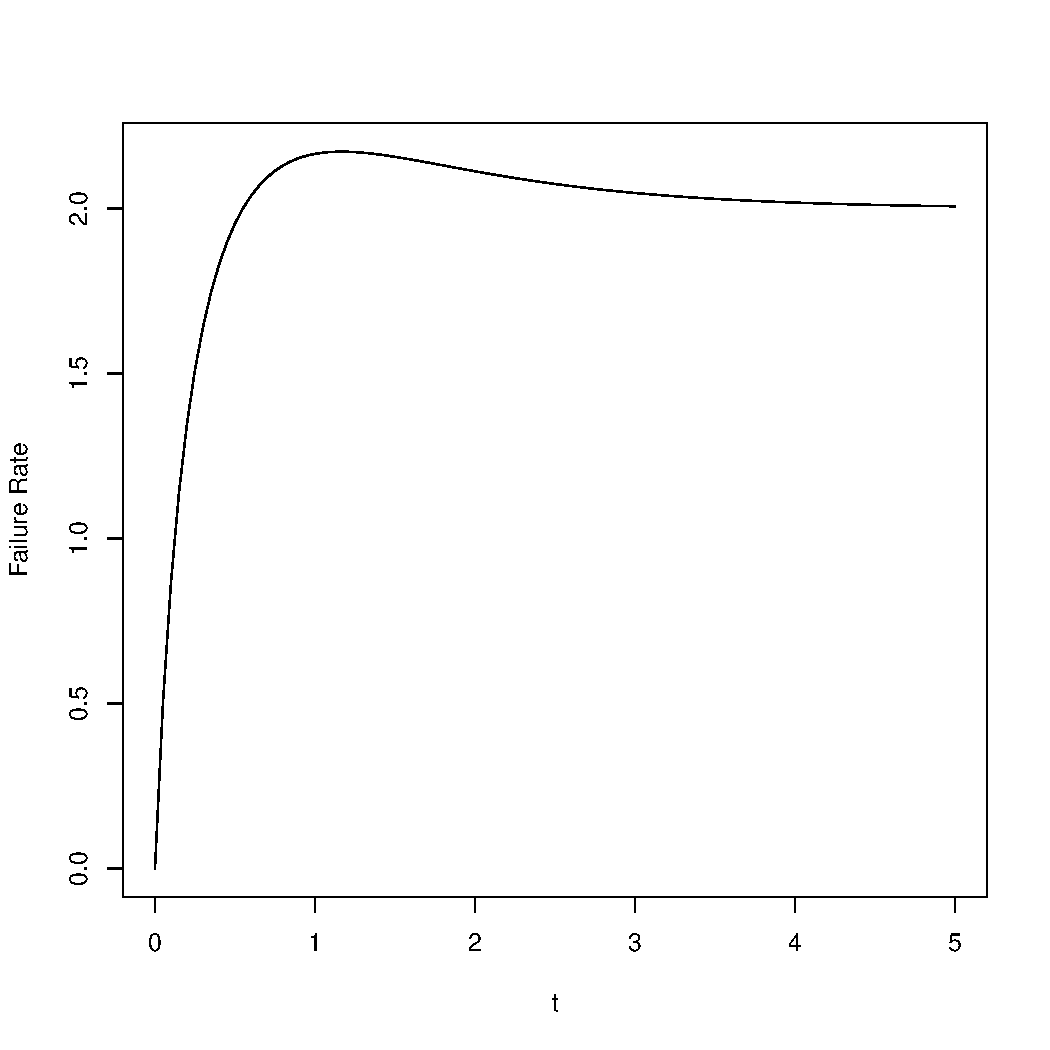
\includegraphics[width=0.5\linewidth]{art/hazard}
\caption{Failure rate of the parallel exponential component system.}
\label{fig:hazard_non_monotone}
\end{figure}





\begin{example}[Weibull Hazard]
The Weibull distribution is very common in reliability analysis since it is tractable generalization of the exponential distribution with many nice properties. 
It can be constructed by 
$\T := \lambda \U^{1/k}$, where $\U \sim \exp(1)$. 
This implies that for non negative $t$:
\begin{align}
	\pdf{\T}{t} &= \frac{k}{\lambda}\left(\frac{\T}{\lambda} \right)^{k-1} e^{-(\T/\lambda)^k}, \\
	\cdf{\T}{t} &= 1 - e^{-(\T/\lambda)^k},
\end{align}
so that 
\begin{align}
	\survive{\T}{t} &= e^ {-(\T/\lambda )^k}, \\
	\hazard{\T}{t} &= \frac{k}{\lambda} \left(\frac{\T}{\lambda} \right)^{k-1} .
\end{align}
\end{example}
Elementary analysis shows that the hazard function of the Weibull may be increasing or decreasing in time ($\T$), depending on $k$, but it is always monotone.




\begin{example}[Empirical risk rates]
When examining empirical risk rates of true devices, we almost always notice a \emph{bathtub} structure, such as in Figure~\ref{fig:bathtub}.\marginnote{Bathtub}
This shape captures the idea that products tend to fail more when they are brand new, or as they are very old, while their failure rates are fairly stable in the ``mid-life''.
In this text, we will not be providing a particular distribution which has this property. 
We refer the reader to \cite{nadarajah_bathtub-shaped_2008} for examples of distributions which have the bathtub property.
\end{example}


\begin{figure}[ht]
\centering
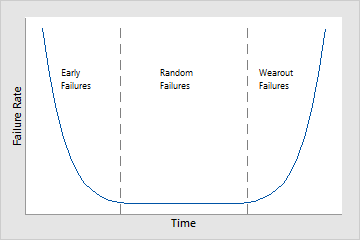
\includegraphics[width=0.5\linewidth]{art/bathtub_curve}
\caption[Bathtub empirical hazard curve]{Bathtub curve of empirical failure rates. \newline
\url{http://support.minitab.com/en-us/minitab/17/topic-library/modeling-statistics/reliability/distributions-in-reliability-analysis/hazard-functions/}}
\label{fig:bathtub}
\end{figure}




\subsubsection{Aging}
The idea of \emph{aging} is that failure rate may vary over time. It is an important concept in reliability, as demonstrated by the empirical bathtub failure rate (Figure~\ref{fig:bathtub}).
Instead of checking if a particular textbook distribution has some ageing property, we instead analyze classes of distributions with the desired notion of ageing.
Our goal will ultimately be to understand the ageing of a whole system, as a function of the ageing of its components.

\begin{definition}[IFR]
We call a failure time distribution to be in the \emph{increasing failure rate} (IFR) ageing class, if it has a non decreasing failure rate.
\end{definition}


\begin{definition}[IFRA]
We call a failure time distribution to be in the \emph{increasing failure rate average} (IFRA) ageing class, if 
$\cuhazard{\T}{t}/t$ is non decreasing in $t$.
\end{definition}
The intuition underlying IFRA relies on understanding $\cuhazard{\T}{t}/t$, which can be seen as the average risk from ignition to time $t$. 
IFRA thus means that even if the risk decreases at some point in time, the average risk still increases. 


\begin{definition}[NBU]
We call a failure time distribution to be in the \emph{new better then used} (NBU) ageing class, if 
$\survive{\T}{t_1+t_2} \leq \survive{\T}{t_2} \survive{\T}{t_1}$.
\end{definition}


\begin{definition}[NBUE]
Define the \emph{expected residual life}, $\mu(t)$, to be 
$$\mu(t):= \expect{\T-t|\T>t}.$$
\marginnote{Expected Residual Life}
We call a failure time distribution to be in the \emph{new better then used in expectation} (NBUE) ageing class, if 
$\mu(t) \leq \mu(0)$.
\end{definition}
NBUE can be easily understood, since it means that a component's expected life is maximal when it is brand new. 


\begin{theorem}
$IFR \Rightarrow IFRA \Rightarrow NBU \Rightarrow NBUE. $
\end{theorem}


The following theorem states a relation between the ageing properties of particular components, and that of the whole system. In particular it states that for the (very wide) class of monotone systems, then the IFRA property is conserved. 
This should be contrasted with the IFR property, which is not conserved, as demonstrated by the parallel system in  Example~\ref{eg:failure_parallel}.
\begin{theorem}[IFRA closure theorem]
\label{thm:ifra_closure}
If the independent components of a monotone system are IFRA, then so is the whole system.
\end{theorem}


Series systems are a extremely small and particular subset of monotone systems.
It does provide, however, an example of systems where not only IFRA is preserved, but also the stronger IFR.
The following corollary follows immediately from Theorem~\ref{thm:ifr_closure} and the fact that a sum of monotone functions is monotone.
\begin{cor}[IFR closure for series systems]
\label{cor:ifr_series}
A series system of independent IFR components is IFR.
\end{cor}




Now consider a two-component system, where one component kicks-in when the first fails.
We will call this an \emph{offline backup}.\marginnote{Offline Backup}
The survival times of the components in an offline backup system are clearly dependent. 
It turns out that for such a system of IFR components, does conserve the IFR property, as seen in the following theorem.
\begin{theorem}[Convolution of IFR]
\label{thm:ifr_convolution}
For two independent random variables, $\x$ and $\y$, both in the IFR ageing class, then so is $\x+\y$.
\end{theorem}
The theorem is called the convolution theorem, because the distribution of a sum of independent random variables, is the convolution of their distributions.


\begin{extra}[IFR and log-concave]
The IFR requirement, is essentially the same as log-concavity of the density function.
This immediately implies many properties of the class, including the convolution theorem above.
See \cite{bagnoli_log-concave_2005}.
\end{extra}

\begin{example}[IFR of Gamma]
The Gamma (and thus the Erlang) distribution is in the IFR aging class, since it is the sum of exponentials, each IFR.
\end{example}

\begin{example}[Series system of offline backups]
What can we say about the ageing class of a series systems of offline backup systems? 
It turns out that if the components are IFR, then so will the whole system.
This is immediate from Corollary~\ref{cor:ifr_series} and Theorem~\ref{thm:ifr_convolution}.
\end{example}






\section{Statistical Analysis}
The probabilistic analysis of the previous section is great fun and all, but like any probabilistic problem, is has to be calibrated to real life. 
This is where data, and statistics come in.
Indeed, given any particular probabilistic model, we may write the likelihood problem, and call upon maximum likelihood principles for estimation.

Failure data and models introduces particular statistical challenges:
\begin{description}
\item [Identifiability] It is typically hard, if not impossible, to estimate the reliability of particular components, from the reliability of the whole system. 
\item [Censoring] A major concern with reliability data, is that in any finite length experiment, some events will just not have happened yet; their failure time will thus be \emph{censored}. Ironically- the more reliable a component, the less data we will have to estimate its reliability. 
\item [Lab versus real-life conditions] Reliable components take very long time to fail. We will thus extrapolate from harsh lab conditions to real-life operating conditions. This requires the introduction of covariates. 
\item [Failure Distribution] like any statistical model, we will need to commit to some failure time sampling distribution.
\end{description}


\subsection{Identifiability}

\begin{example}[Likelihood estimation of a series system]
\label{eg:likelihood_of_failures}
Assume a series system $\Phi$ with $p$ independent, exponential components with rates $(\lambda_1,\dots,\lambda_p)$.
We have $n$ observations on the failure times of the system $t_1,\dots,t_n$.
How can we estimate the failure rates?
To use a likelihood approach, we need the data's sampling distribution.
Denoting the failure time of the $j$'th component of the $i$th device with $\T_{i,j}$, we have that $\T_{i,j}\sim \exp(\lambda_j)$ by assumption.
Since the system is serial, then $\T_i=\min_j(\T_{i,1},\dots,\T_{i,p})$.
By the properties of the exponential distribution $\T_i \sim \exp(\lambda)$, where $\lambda:=\sum_{j=1}^{p} \lambda_j$, as we have already seen with the failure rate. It follows that
$\pdf{\T_i}{t}=\lambda \exp(-\lambda t)$.
We may then write the likelihood function, maximize it with respect to $\lambda$ and discover, as we already know, that $$\hat{\lambda}=\frac{n}{\sum_{i=1}^{n} t_i}.$$
We are now left with the problem of recovering $(\lambda_1,\dots,\lambda_p)$ from $\lambda$. 
Can we do it? On the face of it- no. Which should not surprise us, since the mere knowledge of a device failure, is not very informative on the particular component that failed, which we would need to estimate $(\lambda_1,\dots,\lambda_p)$.
\end{example}

Example~\ref{eg:likelihood_of_failures} teaches us that unless further assumptions are introduced, the estimation of the component-wise failure rates requires information on the component-wise failure times. 





\subsection{Censored Events}
Consider several components being analyze for their reliability. 
Ironically, we actually want them to fail. If they do not, they do not convey information on their reliability.
In the event that a component has not failed, we clearly cannot register its failure time. Omitting this component from the sample will upward bias the estimated reliability.
These events are called \emph{censored} observations. 
There are several types of censoring which depend on the design of the study and the type of event recorded. 
They are all dealt with careful though on the sampling distribution of the data, and the probability of a censoring event. 

Design considerations:
\begin{description}
\item [Type I] occurs when the design is such that the sampling time is fixed a-priori. This implies that the number of failures (thus censoring) events is random. 
\item [Type II] occurs when the design is such that the number of failures (thus censoring) is fixed a-priori. This implies that the sampling duration is random.
\end{description}
If all we know on a censored event is that the actual lifetime is larger then the observation period, we call this a \emph{non-informative} censoring. 
Both designs will then lead to the same modelling of the censoring event, which is now described.

The likelihood function of non-censored events is given by
\begin{align}
	\lik_i=\density_\T(t_i)= \survive{\T}{t_i} \hazard{\T}{t_i},
\end{align}
and the likelihood of a censored event, under the \emph{non-informative} assumption, is given by 
\begin{align}
	\lik_i=\survive{\T}{t_i} .
\end{align}
Unifying the two cases assuming independent observations, using an indicator for censoring, $c_i$, and taking logs we have
\begin{align}
	\loglik &=\log \lik\\ 
	&= \log \prod_{i=1}^{n} \lik_i \\
	&= \log \prod_{i=1}^{n} \survive{\T}{t_i} \hazard{\T}{t_i}^{c_i} \\
	&= \sum_{i=1}^{n} [c_i \log \hazard{\T}{t_i} - \cuhazard{\T}{t_i}]. \label{eq:censored_likelihood}
\end{align}


\begin{example}[Censored exponential lifetimes]
Recalling that the failure rates of exponential lifetimes are fixed, we have that the likelihood of censored exponential lifetimes is given by 
$$
	\sum_{i=1}^{n} [c_i \log \lambda - \lambda t_i].
$$
The maximum likelihood estimator of $\lambda$ is thus
\begin{align}
	\estim{\lambda}= \frac{\sum c_i}{\sum t_i}. \label{eq:censored_ml}
\end{align}
Eq.(\ref{eq:censored_ml}) lends itself to a nice interpretation.
The nominator is the total number of failures.
The denominator is the total \emph{exposure time}. 
The estimated failure rate is thus the number of failures per unit of exposure time. 
\end{example}




\begin{extra}
The previous result is obvious is you consider failures as events which come as a Poisson process, which is implied from the exponential times assumption. 
The process is run for $\sum t_i$ time, and the total event count is $\sum c_i$. 
The trivial estimator for the rate of the process, is $\sum c_i/\sum t_i$.
\end{extra}






\subsection{Accelerated Life Models}
An \emph{accelerate life} model assumes that covariates rescale time. 
For instance, the lab may produce conditions where time advances ten times faster than in real-life operating conditions.
To introduce the model, we start with a simple two group example.
\begin{example}[Two group accelerated life]
\label{eg:two_group_accelerated_life}
Consider two groups indexed by a single dummy variable $x \in \set{0,1}$.
Assuming an accelerated life effect we have
$$
	\survive{\T|x=1}{t} = \survive{\T|x = 0}{t/exp(\beta)} = \survive{\T|x = 0}{t/\gamma}, 
$$
where $\gamma$ is simply shorthand notation for $exp(\beta)$. 
If $\gamma=1/2$, this means that time for group $x=1$ advances twice as fast as for group $x_i=0$.
\end{example}

We now generalize the idea for multiple covariates.
If $\T_1$ is the (random) time to failure under conditions $x_1=(x_{1,1},\dots,x_{1,p})$ , and $\T_0$ under conditions $x_0=(x_{0,1},\dots,x_{0,p})$, we have
\begin{align}
\label{eq:accelerated_life}
	\survive{\T_1}{t}=\survive{\T_0}{t/\gamma},
\end{align}
where $\gamma= e^{(x_1-x_0)' \beta}$, meaning that the conditions $x_1$ are such that time is accelerated by $1/\gamma$ compared to the base conditions $x_0$.
Example \ref{eg:two_group_accelerated_life} is recovered by setting $x_1=1$ and $x_0=0$. 
If $\gamma>1$, time under conditions $x_1$ advances slower than under $x_0$, and the product is expected to live longer. 
The converse holds if $\gamma<1$.


An equivalent formulation of an accelerated life model, which also explains the appearance of the exponent in the time rescaling, is the following 
\begin{align}
\label{eq:estimating_accelerated_life}
	\log \T_i = x_i'\beta + \varepsilon_i,
\end{align}
for some error term $\varepsilon_i$. 
For interpretation, we again denote $e^{x_i'\beta}= \gamma_i$, and infer that $x_i$ accelerates time by $1/\gamma_i$ compared to some base rate where $e^{x_i'\beta}= 1$.
This formulation is more tractable for mathematical manipulation, but conceals the nice interpretation which motivates the model's name.

Eq.(\ref{eq:estimating_accelerated_life}) readily reveals how we can easily estimate the effects ($\beta$) of an accelerate life model.
We simply take the log of the survival times ($\log t_i$), and assuming the particular distribution of $\varepsilon_i$, we may estimate $\beta$ using maximum likelihood.

For future use, we also note that the relation between hazed function under the accelerated life assumption is given by
\begin{align}
\label{eq:hazard_accelerated_life}
		\hazard{\T|x=x_1}{t}=\hazard{\T|x=x_0}{t/\gamma}/ \gamma
\end{align}
where as usual $\gamma=e^{(x_1-x_0)'\beta}$.


\begin{example}[Accelerated life with Gaussian noise]
\label{eg:accelerated_gaussian}
The maximum likelihood estimation of $\beta$ when assuming that $\varepsilon_i \sim \gauss{0,\sigma^2}$, collapses to a simple linear regression when the dependent variable is simply $\log t_i$.
\end{example}


\begin{extra}[Tobit regression]
Assuming $\varepsilon_i \sim \gauss{0,\sigma^2}$, as in the previous example, implies that failure times are \emph{log normal} distributed. 
This approach is known as \emph{Tobit} regression.
\end{extra}


\begin{extra}[Accelerated life with extreme value noise]
\label{eg:accelerated_exponential}
\marginnote{Extreme Value Distribution}
Assuming that the density of $\varepsilon$ is given by 
$$
	\density(\varepsilon)=e^{(\varepsilon-e^\varepsilon)}, 
$$
which is known as an \emph{extreme value distribution}, then failure times have an exponential distribution, and estimation of $\beta$ collapses to an exponential regression problem.
\end{extra}



\begin{extra}
Popular accelerated time models that capture effects of temperature include the \emph{Arrhenius model}, and the \emph{Eyring model}.\marginnote{Arrhenius \\ Eyring}
For models for stress, voltage, humidity, and other life accelerating covariates, see \cite[Sec.8.1.5]{natrella_nist/sematech_2010}
\end{extra}






\subsection{Proportional Hazard Models}
The \emph{proportional hazard}, or \emph{proportional risk} class of models, assumes that covariates multiply not time, but rather failure rates. 
Put differently, accelerated life acts linearly on time, thus non-linearly on hazards. Proportional hazards acts linear on hazards, thus non linearly on time. 
Qualitatively, both either accelerate (decelerate) time. 
Quantitatively, the exact amount of acceleration (deceleration) may differ. 
The choice between these models typically depends on the underlying physical theory, and on the ease of computation and interpretation.

Starting with a two group example
\begin{example}[Proportional hazards in a two group model]
\label{eg:two_group_proportional_hazard}
Consider two groups indexed by a single dummy variable $x \in \set{0,1}$.
Assuming proportional hazard effect we have
$$
	\hazard{\T|x=1}{t}=\hazard{\T|x=0}{t} e^\beta=\hazard{\T|x=0}{t} \gamma, 
$$
where $\gamma$ is again shorthand notation for $e^\beta$.
If $\gamma=1/2$, this means that at any point in time, group $x=1$ suffers half the risk of group $x=0$.
\end{example}


Now for the general case, which compares the risk function under conditions $x=x_1$ to the risk under some base operating conditions $x=x_0$.
\begin{align}
\label{eq:proportional_hazard}
	\hazard{\T|x_1}{t}:=\hazard{\T|x_0}{t} e^{(x_1-x_0)'\beta} = \hazard{\T|x_0}{t} \gamma ,
\end{align}
where $\hazard{\T|x_0}{t}$ is some assumed baseline hazard rate, and $\gamma$ is short notation for $e^{(x_1-x_0)'\beta}$.
Example \ref{eg:two_group_proportional_hazard} is recovered by setting $x_1=1$ and $x_0=0$.


The linear rescaling of the risk in the proportional hazard model, implies the following relation between survival functions
\begin{align}
\label{eq:survival_proportional_hazard}
	\survive{\T|x_1}{t}=\survive{\T|x_0}{t}^{\exp((x_1-x_0)'\beta)}.
\end{align}
To see this recall Eq.(\ref{eq:survival_to_hazard}):
\begin{align*}
\hazard{\T|x_1}{t} 
&=  - \frac{\partial}{\partial t} \log \survive{\T|x_1}{t}  \\
&= - \frac{\partial}{\partial t} \log \survive{\T|x_0}{t}^{\exp((x_1-x_0)'\beta)} \\
&= e^{(x_1-x_0)'\beta} - \frac{\partial}{\partial t}  \log \survive{\T|x_0}{t} \\
&=  \hazard{\T|x_0}{t} e^{(x_1-x_0)'\beta} 
\end{align*}
as required.




\begin{example}[Comparing survival rates in the two group model]
\label{eg:two_groups_two_time_scalings}
We now compare the proportional hazard assumption, versus the accelerated time assumption in the simple two group model. 
Under the accelerated time model, we have (by assumption):
$\survive{\T|x=1}{t} = \survive{\T|x = 0}{t/\gamma}$. 
Under the proportional hazard model, we have (by Eq.(\ref{eq:survival_proportional_hazard})) 
$	\survive{\T|x=1}{t}=(\survive{\T|x=0}{t})^{\gamma}$.
To visualize the difference between the groups we choose some arbitrary distribution (Weibull) and rescale it with $\gamma=2$ under the different models. 
The result is depicted in Figure~\ref{fig:time_rescaling}, from which we see that the same assumed effect $\gamma=e^\beta=2$, acts in opposite directions under the different models. 
This is also evident when examining the simple exponential case, using Eq.(\ref{eq:proportional_hazard}) and Eq.(\ref{eq:hazard_accelerated_life}): under the proportional hazard the risk increases, whereas under accelerated time the risk decreases.

\begin{figure}[ht]
\centering
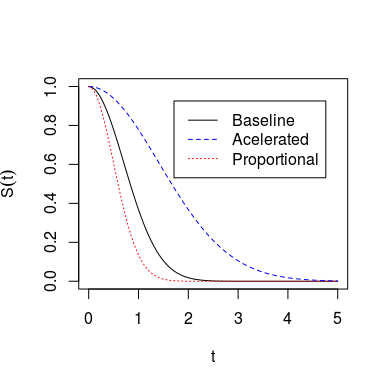
\includegraphics[height=0.3\textheight]{art/survivals}
\caption{}
\label{fig:time_rescaling}
\end{figure}
\end{example}
Example~\ref{eg:two_groups_two_time_scalings}  demonstrates that the different models rescale time in different ways (and even in opposite directions!). 
The example may help you in interpreting the coefficients ($\beta$) of the model you chose. 
In particular it means that a factor with a positive effect ($\hat{\beta}>0$) means accelerated ageing under proportional hazard, and decelerated ageing under accelerated time.


\begin{example}[Accelerated life and proportional hazard for exponential failure times]
Recall that the exponential distribution has a fixed failure rate (over time). 
Using Eq.(\ref{eq:hazard_accelerated_life}) for the accelerated life, and Eq.(\ref{eq:proportional_hazard}) for the proportional hazards, we see that the hazard after any such time rescaling, is still constant in time. 
The exponential distribution, rescaled under any of these models, will still return an exponential distribution.
To se why this is not trivial, you can you your favourite (non negative, continuous) distribution, and check if the hazard function remains in the same class of distributions after a proportional hazard or accelerated life rescaling of time.
\end{example}


\begin{example}[Two groups with exponential baseline]
To demonstrate the previous example, we return to our two group model.
We assume: 
(a) a proportional hazard effect.
(b) an exponential failure time distribution as baseline.
From (b) we have that $\T_{x=0}\sim exp(\lambda) \Rightarrow \hazard{\T|x=0}{t}=\lambda$. 
From (a) we have that $\hazard{\T|x=1}{t}=\gamma \hazard{\T|x=0}{t}= \gamma \lambda \Rightarrow \T_{x=1}\sim exp(\gamma \lambda) $.
We may now collect survival data under the two operating condition, and estimate $(\gamma, \lambda)$, say, with a maximum likelihood estimator. 
\end{example}






\begin{extra}[General Hazard Rate Model]
The effects of covariates on the failure time distribution, may be modelled in many ways. 
The two models presented are probably the most popular, but may certainly be extended. 
For a more detailed discussion, see \cite{cox_analysis_1984}.
\end{extra}





\subsection{Choosing the Base Failure Rate}
In all the above models, we are free to choose the base failure rate: 
$\survive{\T_0}{t}$ in Eq.(\ref{eq:accelerated_life}), or
$\varepsilon$ in Eq.(\ref{eq:estimating_accelerated_life}), or 
$\hazard{\T|x_0}{t}$ in Eq.(\ref{eq:proportional_hazard}).
Three possible approaches include:
\begin{enumerate}
\item Assume a \textbf{parametric} model, such as exponential times, Weibull times, etc.
\item Assume a \textbf{semi-parametric} model, which can be simply seen as a flexible class of distributions, that has no particular parametric representation. In reliability analysis, the \emph{piece-wise constant} hazard is a popular choice.
\item Do not assume anything on the distribution, known as a \textbf{non-parametric} approach. 
\end{enumerate}
If we assume a particular parametric model, then we may gather failure time data, write the likelihood function, and return failure rate estimates, and covariate effects.
We now focus on the more flexible framework of semi-parametric modelling.


\subsection{The Parametric Case}
A parametric model fitting to failure data, is simply a maximum likelihood problem.
Examples \ref{eg:likelihood_of_failures}, \ref{eg:accelerated_gaussian}, and \ref{eg:accelerated_exponential} demonstrate this. 




\subsection{The Semi Parametric Case}
We now relax the explicit failure time distribution assumption, and adopt a more flexible semi-parametric distribution class, known as the \emph{piecewise exponential class}.\marginnote{Piecewise Exponenitial}
Consider the proportional hazard model:
\begin{align}
	\hazard{\T|x_1}{t}:=\hazard{\T|x_0}{t} \times \exp((x_1-x_0)'\beta).
\end{align}
The model clearly requires some baseline failure rate $\hazard{\T|x_0}{t}$.
A flexible, yet not too flexible assumptions, is that the failure rate is constant in some time intervals:
\begin{align}
	\hazard{0}{t}=h_j \quad \text{if} \quad t\in [\tau_{j-1},\tau_j)
\end{align}
This class of distributions has $J(J-1)$ parameters: $(\tau_1,\dots,\tau_{J-1},h_1,\dots,h_J)$.
We are free to choose $J$. 
Large $J$ are very flexible classes, but will require a lot of failure data to estimate.
Small $J$ are less flexible, but require less data to estimate. 
At the limits, when $J=1$, we are back to exponential failure times. 
At the other limit, where $J \to \infty$, we have an absurdly flexible distribution class, which requires impossibly large amounts of data to estimate.

Since the failure rate is piece-wise constant, the distribution class is known as \emph{piece-wise exponential}.\marginnote{Piecewise Exponential}
It is a rather flexible class of distributions. Figure~\ref{fig:piecewise_exponential} depicts the approximation of the Weibull survival function, using a piece-wise constant hazard function, with $J=3$ and appropriate selected parameters.
\begin{figure}[ht]
\centering
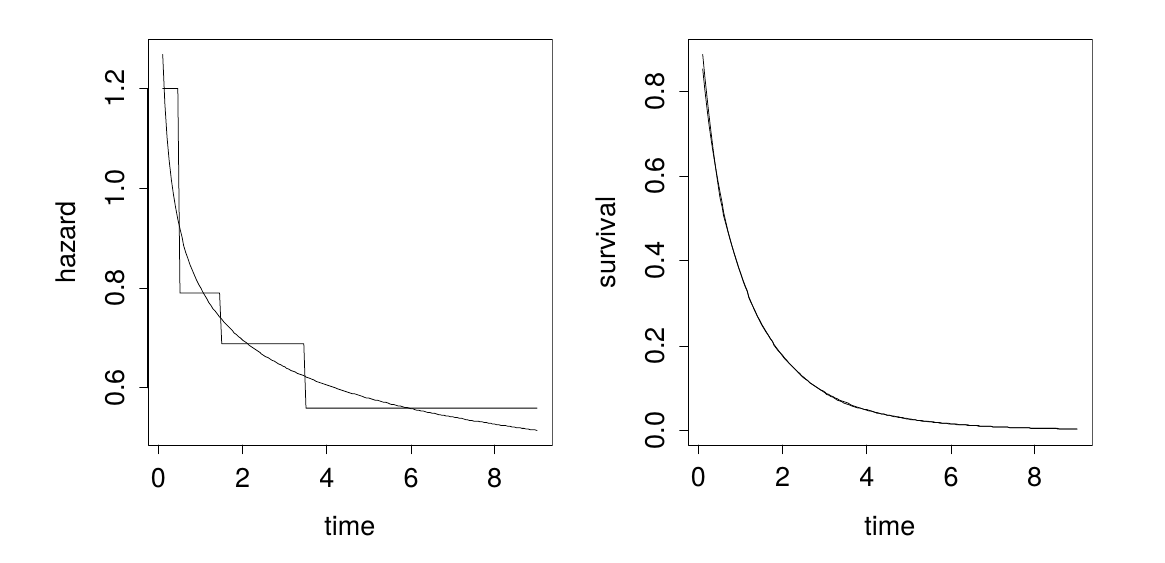
\includegraphics[height=0.2\textheight]{art/piecewise_exponential}
\caption{Piecewise Exponential aproximation of the Weibull distribution.}
\label{fig:piecewise_exponential}
\end{figure}


The piecewise-constant hazard model is very convenient to analyze under the proportional hazard assumption:
\begin{align}
	\hazard{x}{t} = \hazard{x_0}{t} e^{(x-x_0)'\beta} = h_j e^{(x-x_0)'\beta}.
\end{align}
There are $p+2J$ parameters to estimate.
This can be done directly using maximum likelihood, or by casting the problem as several separate Poisson regression problem. 
This has the benefit that the problem may be immediately solved with any statistical software suite, with existing numerical solvers.
We will currently not pursue this avenue, and refer the reader to the bibliographic notes.



\section{Collecting the pieces}
In this chapter we have seen the probabilistic reliability analysis, where we assumed components' reliabilities are known. 
We then proceeded to the statistical problem of estimating reliabilities from failure data.
We now glue collect these pieces to sketch a realistic analysis workflow, which would look roughly as follows:
\begin{enumerate}
\item Estimate reliability parameters by collecting component-wise failure data. Data is collected in a lab so that you may accelerate time and rescale to realistic operating conditions.
\item Perform the probabilistic analysis of the whole system using the estimated parameters.
\end{enumerate}


\begin{remark}[Interplay between probability and statistics]
There is obviously an interplay between the above stages:
In the statistical analysis, we want the least possible set of assumptions;
For the probabilistic analysis, the more we can assume, the more we can say about the system as a whole.
\end{remark}



\begin{remark}[What is a component?]
The notion of a ``system'' and a ``component'' is not well defined.
Indeed, for some purposes you may consider a system, as a component in a larger system.
For the statistical problem, a component is probably the smallest unit you can collect data on. At times, the smallest unit, may be the system as a whole.
\end{remark}




\section{Repairable systems}
In this section we return the a probabilistic analysis.
Unlike the previous sections, we now study systems which may be repaired after they fail.
We will thus want to study the state of the system at time $t$.
This state may depend on the number of failures and repairs performed on the system up to $t$.

We start with the introduction of some quantities of interest.
\begin{definition}[Point availability]
The point availability at time $t$, denoted $A(t)$ is defined as 
\begin{align}
	A(t):= \expect{\Phi_t}=P(\Phi_t=1) .
\end{align}
\end{definition}

\begin{definition}[Interval reliability]
When considering the availability in some time interval $J$, and denoting by $N_J$ the number of system failures in the interval, we may study
\begin{align}
	P(N_j\leq k) &\\
	M(J) &:= \expect{N_j} \\
	A(J) &:= P(\Phi_t=1), \forall t \in J.
\end{align}
\end{definition}


\begin{definition}[Interval downtime]
Denoting by $Y_J=\int_J (1-\Phi_t) dt$ the downtime during interval $J$, we may study
\begin{align}
	P(Y_j \leq y) &	\\
	A^D(J) := \frac{\expect{Y_J}}{|J|}
\end{align}
\end{definition}

\paragraph{Limiting measures} The particular time $t$, or interval $J$ are usually not of real importance in the sense that all times and intervals are equally important.
We will thus typically be interested in the above performance measures for in some \emph{steady state} of the systems, so that the measure is representative of all $t$ (or $J$), and thus no longer depends on $t$ (or $J$).
The typical approach for this is to study the limit of the performance measure, which implies the system has reached it's steady state. Formally, this means studying $\lim_{t \to \infty}$ of the above measures. 


We now start with the analysis of a \emph{single component} system, which we later complicate into \emph{multiple component systems}. 
The required theory is that of stochastic processes, in particular \emph{counting processes}. 
The reader is referred to the bibliographic notes for rigorous proofs and details. 

\subsection{Single component systems}
For a single component, $\Phi_t=\x(t)$. 
If the component fails, it is replaced or repaired. 
We denote by $T_k$ and $R_k$ and the (random) time of the $k$'th run, and repair, respectively.
We assume $T_k \sim F$ and $R_k \sim G$, independent.

\begin{definition}[MTTF]
We denote by $\mu_F=\expect{T_k}$, the \emph{mean time to failure} (MTTF).
\end{definition}


\begin{definition}[MTTR]
We denote by $\mu_G=\expect{R_k}$, the \emph{mean time to repair} (MTTR).
\end{definition}

Obviously, MTTR and MTTF are important characteristics of the single-component system.


\begin{theorem}[Stable point availability]
As $t \to \infty$
\begin{align}
	A(t) \to \frac{\mu_F}{\mu_F+\mu_G}.
\end{align}
\end{theorem}

\begin{theorem}[Stable failures per unit of time]

As $t \to \infty$, then with probability one
\begin{align}
	\frac{N_t}{t} \to \frac{1}{\mu_F+\mu_g}
\end{align}
\end{theorem}

\begin{theorem}[Stable unavailability]
As $t \to \infty$, then with probability one
\begin{align}
	A^D([0,t])=\frac{Y_t}{t} \to \frac{\mu_G}{\mu_F+\mu_G} 
\end{align}

\end{theorem}








\subsection{Multiple component systems}
We will now want to study the availability of a system of multiple repairable components.
The performance of the single-component system still apply, but the analysis now has to account for the fact that the state of the systems depends on the state of $n$ repairable components, assumingly independent.
By indexing the components with $i$, we denote $T_{i,k}, R_{i,k}$ for the uptime and repair time of the $k$'th failure of the $i$'th component. Their distributions are $F_i$ and $G_i$ respectively.
The system failures up to time $t$ is still $N(t)$, but not we also allow for component-wise processes $N_i(t)$, with expectations $M(t)$, and $M_i(t)$.

Denoting $A_i(t)$ the availability of component $i$ at time $t$, $A(t)$ the n-vector of reliabilities, and $A_\Phi(t)$ the whole system's reliability. 

[TODO:Complete from  \cite[Sec.4.3]{aven_stochastic_1999}]



\section{Bibliographic Notes}
An light introductory discussion, may be found in \cite{nahmias_production_2015}. 
The probabilistic analysis in this text is adapted from \cite{aven_stochastic_1999}.
The seminal reference probably being \cite{barlow_mathematical_1965}.
The statistical analysis is adapted from German Rodriguez's Generalized-Linear-Models class notes\footnote{\url{http://data.princeton.edu/wws509/notes/c7.pdf}.} and \cite[Ch.8]{natrella_nist/sematech_2010}.
For more on the statistical analysis, see \cite{cox_analysis_1984}, \cite{kalbfleisch_statistical_2002}, or \cite{klein_survival_2005}.


% 




\chapter{Revisiting System Capability Analysis}
\label{sec:advanced_capability_analysis}
[TODO]
\section{System Capability with Control Charts}
\section{System Capability with Designed Experiments}




\newpage

\appendix




\chapter{Notation}
\label{apx:notation}

In this text we use the following notation conventions:
\begin{description}
\item[$x$] A column vector, or scalar, as implied by the text. 
\item[$:=$] An assignment, or definition. $A:=a$ means that $A$ is defined to be $a$. 
\item[$\prod_{i=1}^{n}$] The product operator: $\prod_{i=1}^{n} x_i:= x_1 \times \dots \times x_n$.
\item[$\coprod_{i=1}^{n}$] The coproduct operator: $\coprod_{i=1}^{n} x_i:= 1-(1-x_1) \times \dots \times (1-x_n)$.
\item[$\#\set{A}$] The count operator. Returns the number of elements of the set $A$. Also known as the \emph{cardinality}.
\item[$\Phi(t)$] The standard Gaussian CDF at $t$: $\Phi(t):= P(Z<t)$.
\item[$\phi(t)$] The standard Gaussian density at $t$: $\phi(t):= \frac{\partial}{\partial t}\Phi(t)$.
\item[$x'$] We use $'$ for the transpose operation. For a $1\times p$ row vector $x$, then $x'$ is a $p \times 1$ column vector.
\item[$\x_n \rightsquigarrow \dist$] Convergence in distribution: for large enough $n$, then $\x_n$ is distributed like $\dist$.
\item[$\conv$] The convolution operator: $f \conv g=(f \conv g)(t)=\int f(s) g(t-s) ds$.
\item[$f^{\conv n}$] The convolution power: $n$ convolutions of $f$ with itself.
\end{description}


 



\chapter{R}
\label{apx:r}

\begin{description}
\item [Exploratory] See, for instance, \cite{venables_modern_2002}, or any of the endless free web resources. 
\item [Inference] The same as exploratory.
\item [SPC] For SPC with R see the \rcode{qcc}, \rcode{spc} packages, the appendix in \cite{qiu_introduction_2013}, and here \\ \url{http://blog.yhathq.com/posts/quality-control-in-r.html}.
\item [DOE] For DOE with \R, see \\ \url{https://cran.r-project.org/web/views/ExperimentalDesign.html}.
\item [Reliability] For DOE with \R, see \\ \url{https://cran.r-project.org/web/views/Survival.html}
\end{description}


 


\newpage
\addcontentsline{toc}{chapter}{Bibliography}
\bibliographystyle{abbrvnat_JR}
\bibliography{QualityEngineering}
\label{sec:bibliography}


\end{document}